\documentclass[10pt,openany]{book}
\usepackage{ctex} 
\usepackage{geometry,graphicx,xcolor,color,hyperref}
\usepackage{tcolorbox}

\geometry{
  a4paper,
  top=25.4mm, bottom=25.4mm,
  left=20mm, right=20mm,
  headheight=2.17cm,
  headsep=4mm,
  footskip=12mm
}

\usepackage{amssymb,amsmath,mathrsfs}                    % 数学字体
\usepackage{mathpazo}% 采用 Palatino 风格字体
\usepackage[nofontspec]{newpxtext}
\setcounter{tocdepth}{1}%目录显示到第一级,section
\setcounter{secnumdepth}{2}%编号到第二级,subsection
\definecolor{winered}{rgb}{0.5,0,0}
\definecolor{structurecolor}{RGB}{122,122,142}
\definecolor{main}{HTML}{3D445F}
\definecolor{second}{HTML}{627581}
\definecolor{third}{HTML}{9D8798}
% 定义引用的颜色
\hypersetup{colorlinks = true, linktoc=all, linkcolor=black, urlcolor=winered}

% ------------------------------------------------------------%
% 定义定理环境
\usepackage{amsthm}
\newtheoremstyle{defstyle}{3pt}{3pt}{\kaishu}{-3pt}{\bfseries\color{main}}{}{0.5em}{\indent 【\thmname{#1} \thmnumber{#2}】 \thmnote{(#3)}}
\newtheoremstyle{thmstyle}{3pt}{3pt}{\kaishu}{-3pt}{\bfseries\color{second}}{}{0.5em}{\indent【\thmname{#1} \thmnumber{#2}】 \thmnote{(#3)}}
\newtheoremstyle{prostyle}{3pt}{3pt}{\kaishu}{-3pt}{\bfseries\color{third}}{}{0.5em}{\indent【\thmname{#1} \thmnumber{#2}】 \thmnote{(#3)}}

\theoremstyle{thmstyle} %theorem style
  \newtheorem{theorem}{定理}[chapter]
\theoremstyle{defstyle} % definition style
  \newtheorem{definition}[theorem]{定义}
  \newtheorem{lemma}[theorem]{引理}
  \newtheorem{corollary}[theorem]{推论}
\theoremstyle{prostyle} % proposition style
  \newtheorem{proposition}[theorem]{命题}
  \newtheorem{example}[theorem]{例题}
  \newtheorem{remark}[theorem]{注}

\renewenvironment{proof}[1][证明]{\par\underline{\textbf{#1.}} \;\fangsong}{\qed\par}
\newenvironment{solution}{\par\underline{\textbf{解.}} \;\kaishu}{\qed\par}
\newcommand{\intro}[1]{\rightline{\parbox[t]{5cm}{\footnotesize \fangsong\quad\quad #1 }}}
% ------------------------------------------------------------%
% ------------------------------------------------------------%
% 设置章形式
\usepackage{titlesec, titletoc}
\linespread{1.2} 				
\usepackage{fancyhdr}
\fancyhf{}
\renewcommand{\headrule}{\color{structurecolor}\hrule width\textwidth}
\pagestyle{fancy}
\renewcommand{\headrulewidth}{1pt}
\fancypagestyle{plain}{\renewcommand{\headrulewidth}{0pt}\fancyhf{}\renewcommand{\headrule}{}}

\fancyhead[c]{\color{structurecolor}\kaishu\rightmark}
\fancyfoot[c]{\color{structurecolor}\small\thepage}

\titleformat{\chapter}[display]{\Large}
{\color{structurecolor}\filleft
\parbox{1cm}{\vbox to 1.5cm{\vfill\hbox to 4cm{\hfill\Huge \bfseries \color{structurecolor}{Chapter} \thechapter \hfill}}}}
{1ex}
{\color{structurecolor} \titlerule[2pt]\large\bfseries \filright \vspace*{1em}}
[\vspace*{1em} {\titlerule[2pt]}]

\titleformat{\section}[frame]{\normalfont\color{structurecolor}}{\footnotesize \enspace \large \textcolor{structurecolor}{\S \,\thesection}\enspace}{6pt}{\Large\filcenter \bf \kaishu }


\titleformat{\subsection}[hang]{\bfseries}{\large\bfseries\color{structurecolor}\thesubsection\enspace}{1pt}{\color{structurecolor}\large\bfseries\filright}

\titleformat{\subsubsection}[hang]{\bfseries}{\large\bfseries\color{structurecolor}\thesubsubsection\enspace}{1pt}{\color{structurecolor}\large\bfseries\filright}
% ------------------------------------------------------------%
% 设置封面
\usepackage{titling}
\renewcommand*{\maketitle}{
    \begin{titlepage}
    \newgeometry{margin = 0in}
    \parindent=0pt
    \vfill
    \begin{center}
        \parbox{0.618\textwidth}{
        \hfill {\bfseries \Huge \thetitle} \\[0.6pt]  
        \rule{0.618\textwidth}{4pt} \\ 
    }
    \end{center}
    \vfill
    \begin{center}
        \parbox{0.618\textwidth}{
        \hfill\Large
        \kaishu 
          \begin{tabular}{r|}
          作者:Jiang \\ 
          时间:\thedate \\
        \end{tabular}
        }
    \end{center}
    \vfill
    \begin{center}
        \parbox[t]{0.7\textwidth}{\centering \kaishu }
    \end{center}
    \vfill
\end{titlepage}
\restoregeometry
\thispagestyle{empty}
}
% ------------------------------------------------------------%


\title{读书笔记}
\date{\today}

\begin{document}
\frontmatter

\maketitle

\tableofcontents

\mainmatter

\chapter{杂项}
\section{Ginzburg–Landau Theory}
\section{用Chiral symmetry求解一堆pauli矩阵的能谱}
对于并非所有项都是gamma matrix的哈密顿量,无法直接平方求解,此时若存在chiral symmetry,可以简化求解,举一例子:
\begin{equation}
  \begin{aligned}
    H_1(\mathbf{k})= & t_x \tau_1 \sigma_0+\left[-t \cos k_x \gamma_3+t \sin k_x \gamma_4\right. \\
    & \left.+\left(t_y+t \cos k_y\right) \gamma_1-t \sin k_y \gamma_2\right]
    \end{aligned}
\end{equation}

其中哈密顿量$ \gamma_j=\tau_1 \sigma_j \quad(j=1,2,3), \quad \gamma_4=\tau_2 \sigma_0 $, 存在chiral symmetry:$ \mathcal{C}=\tau_3 \sigma_0 $,chiral算符在$ \tau $的基下是对角化的,而哈密顿量应在chiral的本征态基下off block diagonal
\begin{equation*}
  H=\left(\begin{array}{cc}
    0 & D \\
    D^{\dagger} & 0
    \end{array}\right)
\end{equation*}
哈密顿量的本征值为$ \pm \sqrt{\lambda} $,其中$ \lambda $为$ D D^{\dagger} $的本征值。因此可以想到将哈密顿量拆分为$ A\otimes \tau_1 + B\otimes \tau_2 $的形式,此时$ D = A + iB $,此时A、B只包含一个pauli算符,因此可以直接求解。   
\section{Energy-Time Uncertainty Relation}

\section{量子力学的绝热定理}
绝热定理指出,若哈密顿量通过依赖于参数而依赖于时间,当参数改变的足够缓慢且哈密顿的能级之间未发生交错时,$ H(0) $对应第n个本征值的态将也演化到$ H(\lambda(t)) $的第n个本征值对应的本征态。
\subsection*{证明}
考虑一含时哈密顿量与它的含时本征态:
\begin{equation}
	H(t)|n(t)\rangle=E_n(t)|n(t)\rangle
\end{equation}
在任意时间t,这组含时本征态都构成一组完备基,t时刻的态矢总能在这组基下做展开:
\begin{equation}
	|\psi(t)\rangle=\sum_n c_n(t)|n(t)\rangle
\end{equation}
将它带入含时薛定谔方程,得到一个系数满足的方程:
\begin{equation}
	i \hbar \dot{c}_m(t)+i \hbar \sum_n c_n(t)\langle m(t) \mid \dot{n}(t)\rangle=c_m(t) E_m(t)
\end{equation}
为得到右矢对时间的导数,对含时哈密顿量的本征方程对时间求导,并且对$ <m(t)| $做内积,最终有\footnote{若$m=n$,得到$<n|\partial_t H|n> = \partial_t E_n$,推广到一般的参数就是
Hellmann–Feynman定理。若$m\neq n,\langle m(t) \mid \dot{n}(t)\rangle=-\frac{\langle m(t)|\dot{H}(t)| n(t)\rangle}{E_m(t)-E_n(t)}$}:
\begin{equation}
	\dot{c}_m(t)+\left(\frac{i}{\hbar} E_m(t)+\langle m(t) \mid \dot{m}(t)\rangle\right) c_m(t)=\sum_{n \neq m} \frac{\langle m(t)|\dot{H}| n(t)\rangle}{E_m(t)-E_n(t)} c_n(t)
\end{equation} 
上述内容都是exact的,现在考虑绝热近似:假设哈密顿量改变的足够慢且能级不交叉,则可以忽略等式的右边。剩下的方程可以简单解出:
\begin{equation}
	c_m(t)=c_m(0) e^{i \theta_m(t)} e^{i \gamma_m(t)}
\end{equation}
$ \theta $是能量与时间带来的相位,$ \gamma_m(t)=i\int\langle m(t) \mid \dot{m}(t)\rangle dt $是一个几何相位,可以证明它是纯实的,这等价于$ \langle m(t) \mid \dot{m}(t)\rangle $纯虚,这可以从$ \langle m(t) \mid m(t)\rangle =1$,再对时间求导看出。\\

如果以对参数依赖而依赖于时间时,几何相位可以写为:
\begin{equation}
	\gamma_m(t)=i \int_{t_0}^t\left\langle\psi_m(t)\left|\partial_{\vec{R}}\right| \psi_m(t)\right\rangle \dot{\vec{R}} d t^{\prime}=i \int_C\left\langle\psi_m(\vec{R})\left|\partial_{\vec{R}}\right| \psi_m(\vec{R})\right\rangle d \vec{R}
\end{equation}
\section{Berry相位}
\subsection{形式改写}
可以仿照电磁学,定义线积分的矢量为Berry联络,利用Stokes定理,Berry联络的旋度为Berry曲率,Berry相是Berry联络的线积分。可以得到这样的一个Berry相位表达式:
\begin{equation}
	\begin{aligned}
		\gamma_n & \left.=-\operatorname{Im} \int d \mathbf{S} \cdot(\nabla \times\langle n(\mathbf{R})|\nabla| n(\mathbf{R})\rangle)=-\operatorname{lm} \int d S_i \epsilon_{i j k} \nabla_i\left\langle n(\mathbf{R})\left|\nabla_k\right| n(\mathbf{R})\right\rangle\right) \\
		& =-\operatorname{Im} \int d \mathbf{S} \cdot(\langle\nabla n(\mathbf{R})|\times| \nabla n(\mathbf{R})\rangle) .
		\end{aligned}
\end{equation}
但这依赖于规范的,对于电脑计算并不方便,这里给出与规范无关的计算式。考虑对于Berry相的表达式中插入哈密顿量本征态作为完备基,有:
\begin{equation}
	\begin{gathered}
		\left.\epsilon_{i j k}\left\langle\nabla_j n(\mathbf{R})\left|\nabla_k\right| n(\mathbf{R})\right\rangle\right) \\
		\left.\left.=\epsilon_{i j k}\left\langle\nabla_j n(\mathbf{R}) \mid n\right\rangle\left\langle n \mid \nabla_k n(\mathbf{R})\right\rangle\right)+\sum_{m \neq n} \epsilon_{i j k}\left\langle\nabla_j n(\mathbf{R}) \mid m\right\rangle\left\langle m \mid \nabla_k n(\mathbf{R})\right\rangle\right)
		\end{gathered}
\end{equation}
第一项为两个虚数的乘积,为纯实数,所以可以略去,得到Berry相位的表达式:
\begin{equation}
	\begin{gathered}
		\gamma_u=-\iint_{\mathcal{C}} d \mathbf{S} \cdot \mathbf{V}_n \\
		=-\iint_{\mathcal{C}} d \mathbf{S} \cdot \operatorname{Im} \sum_{m \neq n} \frac{\left\langle n(\mathbf{R})\left|\left(\nabla_{\mathbf{R}} H(\mathbf{R})\right)\right| m(\mathbf{R})\right\rangle \times\left\langle m(\mathbf{R})\left|\left(\nabla_{\mathbf{R}} H(\mathbf{R})\right)\right| n(\mathbf{R})\right\rangle}{\left(E_m(\mathbf{R})-E_u(\mathbf{R})\right)^2}
		\end{gathered}
\end{equation}
通过这种方法,原本通过绝热演化而投影掉的非n态又重新回来了,在这个形式中对能级求和,可以发现Berry曲率对所有能级的求和总是零,因此陈数就是零\footnote{研究N能级系统就是参数空间M上的U(N)主从,数学上的一个定理保证了可以通过研究U(N)的陈数来研究$ U(1)^{\times N} $,而U(N)的陈数是零,所以所有能级求和为零 }。上述讨论仍局限于能级无简并。
\subsection{简并与能级交错}
可以看到,当改变参数使得非简并的态之间发生了能级简并时,给出Berry曲率的奇异性。上式只包含了两两之间的能量差,所以一个两能级物理体系就能体现很多问题的核心。这里通过考虑一两能级体系来看看在能量简并点到底发生了什么:对于$ E(\mathbf{R})_+\geq E(\mathbf{R})_- $,在能级简并点$ E(\mathbf{R^*})_+=E(\mathbf{R^*})_- $,将哈密顿量在简并点附近展开为:$H(\mathbf{R}) \approx H\left(\mathbf{R}^*\right)+\left(\mathbf{R}-\mathbf{R}^*\right) \cdot \boldsymbol{\nabla} H\left(\mathbf{R}^*\right)$,这给出Berry曲率:
\begin{equation}
	\mathbf{V}_{+}((\mathbf{R}))=\operatorname{lm} \frac{\left\langle+(\mathbf{R})\left|\left(\nabla H\left(\mathbf{R}^*\right)\right)\right|-(\mathbf{R})\right\rangle \times\left\langle-(\mathbf{R})\left|\left(\nabla H\left(\mathbf{R}^*\right)\right)\right|+(\mathbf{R})\right\rangle}{\left(E_{+}(\mathbf{R})-E_{-}(\mathbf{R})\right)^2} .
\end{equation} 
由于叉乘的反对易性,很容易看出两个能级的Berry曲率刚好为相反数。具体而言,考虑这样一个二能级哈密顿量:$ \hat{H}(\mathbf{d})=d_x \hat{\sigma}_x+d_y \hat{\sigma}_y+d_z \hat{\sigma}_z=\mathbf{d} \cdot \hat{\sigma} $,$\mathbf{d}$。\\

很容易看出,上述哈密顿量的平方正比于单位矩阵,其本征值也很容易得到。利用球坐标将$ \vec{d} $参数化,很容易得到本征矢:
\begin{equation}
	\left|+_{\mathbf{d}}\right\rangle=e^{i \alpha(\theta, \varphi)}\left(\begin{array}{c}
		e^{-i \varphi / 2} \cos \theta / 2 \\
		e^{i \varphi / 2} \sin \theta / 2
		\end{array}\right)
\end{equation}   
对应负本征值的本征矢相应地为:$ \left|-_{\mathbf{d}}\right\rangle=e^{i \beta(\mathbf{d})}\left|+_{-\mathbf{d}}\right\rangle $\\
不难算出,Berry曲率在此问题中为:$ \mathbf{V}_{+}(\mathbf{R})=\frac{\mathbf{R}}{2 R^3} $,具有位于原点处磁单极子的形式,而哈密顿量在参数空间的原点处简并,因此每有一个参数空间的简并点都给出该处的一个磁单极子形式的Berry曲率。 
\subsection{用投影算符计算陈数}
定义第n个能级的投影算符$ P_n(\mathbf{k})=\left|\psi_n(\mathbf{k})\right\rangle\left\langle\psi_n(\mathbf{k})\right| $,可以用它计算陈数
\begin{equation}
  C_n=\frac{1}{2 \pi i} \int d k_x d k_y \operatorname{Tr}\left(P_n\left[\partial_{k_x} P_n, \partial_{k_y} P_n\right]\right)
\end{equation}

为证明这个形式,考虑投影算符对参数的偏导数(之后都略去$ (\mathbf{k}) $与n ),展开上式:
\begin{equation}
  \partial_x (\left|\psi_n(\mathbf{k})\right\rangle\left\langle\psi_n(\mathbf{k})\right|) = 
  \left|\partial_x \psi_n(\mathbf{k})\right\rangle\left\langle \psi_n(\mathbf{k})\right| + \left|\psi_n(\mathbf{k})\right\rangle\left\langle\partial_x\psi_n(\mathbf{k})\right|
\end{equation}
对易子后将产生形如$ \left|\partial_x \psi_n(\mathbf{k})\right\rangle\left\langle \psi_n(\mathbf{k})\right|\left|\partial_y \psi_n(\mathbf{k})\right\rangle\left\langle \psi_n(\mathbf{k})\right| - {x\to y}$的项,利用关系式$ <\partial \psi|\psi> + <\psi|\partial\psi> = 0 $ 现在考察这种项的贡献:
$ Tr{P(\dots)} = 0$,剩下的项显然给出和常见定义的berry curvature相同的项  
\begin{equation}
  \partial_{k_\mu} P_n=\left(\partial_{k_\mu}\left|\psi_n(\mathbf{k})\right\rangle\right)\left\langle\psi_n(\mathbf{k})|+| \psi_n(\mathbf{k})\right\rangle\left(\partial_{k_\mu}\left\langle\psi_n(\mathbf{k})\right|\right), \quad \mu=x, y
\end{equation} 

\subsection{纤维丛的语言}
\section{霍尔电导的量子化}
\subsection{Chern数}
Chern数定义为Berry曲率在整个参数空间的积分,对于紧致的流形,Naive地运用Stokes定理会给出零Chern数,那么非零的Chern数是怎么来的呢?考虑Stokes定理运用的条件,它需要$ A $是在整个参数空间Well-defined的,但很多时候会出现如二能级系统一样的情况,整个参数空间总是无法选取一个连续的规范,此时将参数空间分为多个区域,每个区域中有不同的连续的规范,使得Stokes定理在每个单独的区域内都可以使用。具体而言,考虑参数空间有一个规范奇点,此时选取两个规范:
\begin{equation}
	\mathbf{A}_2(k)=\psi_2 \partial_{\mathbf{k}} \psi_2=\psi_1 \partial_{\mathbf{k}} \psi_1+i \nabla \chi(k)=\mathbf{A}_1(k)+i \nabla_\chi(k)
\end{equation} 
此时Berry曲率在全空间的积分可以分为两部分:
\begin{equation}
	\int_{T_{BZ}^2-R^\epsilon} \nabla \times \mathbf{A}_1(k)+\int_{R^\epsilon} \nabla \times \mathbf{A}_2(k)
\end{equation}
积分曲面共享一个边界,但取向不同,利用Stokes定理得到在边界线积分的差,也即$ \nabla \chi(k) $的回路积分。由于波函数的单值性与积分在一回路上,$ \mathbf{R(0)}=\mathbf{R(T)},|m(\mathbf{R(0)})> =|m(\mathbf{R(T)})>$,回路积分给出$ 2\pi n $,因此对全空间的Berry曲率积分确实非零,且取整数。  
\subsection{Kubo公式}
先考虑电流算符在二次量子化中的形式,我们当然可以通过电荷守恒关系,从电荷密度算符的二次量子化导出电流算符,但这里采取一种更加简单的方式,考虑定义:$ \vec{j}=-\frac{\delta H}{\delta \vec{A}} $,其中H为电磁场下的哈密顿量:
\begin{equation}
	H=\int d^3 x\left[\frac{1}{2 m} \psi^{\dagger}(x)(-i \hbar \vec{\nabla}-e \vec{A}(x))^2 \psi(x)-e \phi(x) \psi^{\dagger}(x) \psi(x)\right]+V_{I N T}
\end{equation} 
不难算出电流算符:$ \vec{j}(x)=-\frac{i e \hbar}{2 m} \psi^{\dagger}(x) \stackrel{\leftrightarrow}{\nabla} \psi(x)-\left(\frac{e^2}{m}\right) \vec{A}(x) \rho(x) $,其中定义了对称导数$ \stackrel{\leftrightarrow}{\nabla}=\frac{1}{2}(\stackrel{\rightarrow}{\nabla}-\stackrel{\leftarrow}{\nabla}) $。电流算符本身是规范不变的,但有时候选取某种规范可以简化问题,因此这驱使我们将电流拆分为部分之和,虽然部分是规范变换的,一种常用的拆分为:$ \vec{j}(x)=\vec{j}_P(x)+\vec{j}_D(x) $,定义为:
\begin{equation}
	\begin{aligned}
		&\vec{j}_P(x)=-\frac{i e \hbar}{m} \psi^{\dagger}(x) \stackrel{\leftrightarrow}{\nabla} \psi(x)\\
		&\vec{j}_D(x)=-\left(\frac{e^2}{m}\right) \vec{A}(x) \rho(x)
		\end{aligned}
\end{equation}   
分别为电流的顺磁项与反磁项。选取Londo规范,$ \nabla \dot \vec{A}=0 $,此时的麦克斯韦方程中电势全由电荷决定,因此在电中性的体系中可以取为零。这种拆分在Londo唯象地描述超导现象时用到了,详情可见Coleman,p336。顺磁项给出了一个简单的对外场的响应,而反磁项则须利用线性响应理论计算,很容易写出:
\begin{equation}
	\begin{aligned}
		\vec{j}(1) & =-\int d 2 \underline{Q}(1-2) \vec{A}(2) \\
		Q^{\alpha \beta}(1-2) & =\frac{n e^2}{m} \delta^{\alpha \beta} \delta(1-2)-i\left\langle\left[j_P^\alpha(1), j_P^\beta(2)\right]\right\rangle \theta\left(t_1-t_2\right)
		\end{aligned}
\end{equation}
在动量空间中的形式即为Kubo公式:
\begin{equation}
	\begin{aligned}
		\vec{j}(q) & =\sigma(q) \vec{E}(q) \\
		\sigma^{\alpha \beta}(q) & =-\frac{1}{i v} Q^{\alpha \beta}(q)=\frac{1}{-i v}\left\{\frac{n e^2}{m} \delta^{\alpha \beta}-i\left\langle\left[j^\alpha(q), j^\beta(-q)\right]\right\rangle\right\}
		\end{aligned}
\end{equation}
频率的倒数来自$ E(q)=\frac{1}{i\nu}A(q) $。\\

实际上很多时候并非从微观哈密顿量算起,而是能带哈密顿量$ H=\sum_{i, j, a, \beta} c_{i a}^{\dagger}\left(h_{i j}^{a \beta}-\mu \delta_{i j} \delta_{a \beta}\right) c_{j \beta} $ 。假设相互作用具有平移不变性:$ h_{i j}=h_{i-j} $,并将哈密顿量写在倒空间:
\begin{equation}
	c_j^a=\frac{1}{\sqrt{N}} \sum_k e^{i k j} c_k^a, \quad H=\sum_k c_{k a}^{\dagger} h_k^{a \beta} c_{k \beta},
\end{equation} 
此时电流算符并非之前的形式,但推导的实质仍是前述的两种:电荷守恒与电磁场下哈密顿量的变分。之后的推导为方便省略轨道指标。
\subsubsection*{连续性条件}
将电荷的连续性条件写在动量空间中:
\begin{equation}
	\dot{\rho}(x)+\nabla \cdot \mathbf{J}(x)=0, \quad \rightarrow \dot{\rho}_q-i \mathbf{q} \cdot \mathbf{J}_q=0
\end{equation}
其中动量空间的密度算符为$ \rho(\mathbf{q})=\frac{1}{\sqrt{N}}\sum_k c^\dagger_{\mathbf{k}+\mathbf{q}}+c_{\mathbf{q}} $。对时间的导数由Heisenberg方程就是和哈密顿量的对易子,因此有:
\begin{equation}
	-i \mathbf{q} \cdot \mathbf{J}_{\mathbf{q}}=-\dot{\rho}_q=i[\rho, H]=i \frac{1}{\sqrt{N}} \sum_{p, k} h_p\left[c_{\mathbf{k}+\mathbf{q}}^{\dagger} c_{\mathbf{k}}, c_p^{\dagger} c_p\right]
\end{equation}
简单的对易关系给出:
\begin{equation}
	\mathbf{q} \cdot \mathbf{J}_{\mathbf{q}}=\frac{1}{\sqrt{N}} \sum_{ k}\left(h_{\mathbf{k}+\mathbf{q}}-h_{\mathbf{k}}\right) c_{\mathbf{k}+\mathbf{q}}^{\dagger} c_{\mathbf{k}}
\end{equation}
对于我们感兴趣的长波极限,也就是说外场的波长远大于原子间的间距时,可以将$ \mathbf{q} $视为小量。平移求和的哑指标$ k\to k-q/2 $,这相当于从向前差分变为中心差分,精度从O(q)提升到O($ q^2 $ ),则有:
\begin{equation}
	\begin{aligned}
		\mathbf{q} \cdot \mathbf{J}_{\mathbf{q}} & =\frac{1}{\sqrt{N}} \sum_{ k}\left(h_{\mathbf{k}+q / 2}-h_{\mathbf{k}-q / 2}\right) c_{\mathbf{k}+q / 2}^{\dagger} c_{\mathbf{k}-q / 2} \\
		& =\frac{1}{\sqrt{N}} \sum_{ k}\left(\frac{\partial h_k}{\partial \mathbf{k}} \cdot \mathbf{q}\right) c_{\mathbf{k}+\frac{\mathbf{q}}{2}}^{\dagger} c_{\mathbf{k}-\frac{\mathbf{q}}{2}}+\mathcal{O}\left(q^2\right)
		\end{aligned}
\end{equation} 
由此得到电流算符为:$ \mathbf{J}_{\mathbf{q}}= \frac{1}{\sqrt{N}} \sum_{ k} c_{\mathbf{k}+\frac{\mathbf{q}}{2}}^{\dagger} \frac{\partial h_k}{\partial \mathbf{k}} c_{\mathbf{k}-\frac{\mathbf{q}}{2}}$。
\subsubsection*{从Peierls替换导出}
已经知道Pererls替换是给跃迁系数乘上一相位,在这相位很小的情况下可以将指数函数展开并保留到一阶项,此时哈密顿量可以分为无磁场项与加磁场新产生的项:
\begin{equation}
	H=\sum_{i, j, a, \beta} c_{i a}^{\dagger} h_{i j}^{a \beta} e^{i \int_j^i \mathbf{A}(l) \cdot d \mathbf{l}} c_{i \beta} \approx \sum_{i, j, a, \beta} c_{i a}^{\dagger} h_{i j}^{a \beta}\left(1+i \int_j^i \mathbf{A}(l) \cdot d \mathbf{l}\right) c_{j \beta}=H_0+H_{\mathrm{ext}},
\end{equation}  
\begin{equation}
	\begin{aligned}
		H_{\mathrm{ext}} & =\sum_{k_1, k_2, a, \beta} c_{k_1, a}^{\dagger} c_{k_2, \beta} \frac{1}{N} \sum_{r, j} e^{i\left(\mathbf{k}_2-\mathbf{k}_1\right) \cdot \mathbf{j}-i \mathbf{k}_1 \cdot \mathbf{r}} h_r^{a \beta} i \int_j^{j+r} \mathbf{A}(l) \cdot d \mathbf{l} \\
		& \approx \sum_{k_1, k_2, a, \beta} c_{k_1, a}^{\dagger} c_{k_2, \beta} \frac{1}{N} \sum_{r, j} e^{i\left(\mathbf{k}_2-\mathbf{k}_1\right) \cdot \mathbf{i}-i \mathbf{k}_1 \cdot \mathbf{r}} h_r^{a \beta} i \mathbf{r} \cdot \mathbf{A}\left(\mathbf{j}+\frac{\mathbf{r}}{2}\right) .
		\end{aligned}
\end{equation}
可以将它在倒空间中写出,对各项都做傅立叶变换,最终有:
\begin{equation}
	H_{\mathrm{ext}}=\sum_{k, q, a, \beta} c_{k+q / 2, a}^{\dagger} c_{k-q / 2, \beta} \frac{\partial h_k^{a \beta}}{\partial \mathbf{k}} \cdot \mathbf{A}_{-q}=\sum_q \mathbf{j}_q \cdot \mathbf{A}_{-q} .
\end{equation}
可以看出这和之前的推导给出一致的结论。\\

对于霍尔效应的电导率推导,我们只关心反磁项,因为顺磁项在空间中对角化,不贡献霍尔电导。
由于实际材料几乎总是Bloch电子,因此实际推导需要利用上面得到的电流算符。现在推导响应函数的形式。我们希望计算外加电磁场以后得电流$ \vec{j}(\vec{x}, t)=\left\langle\vec{j}_P(x, t)\right\rangle-\frac{n e^2}{m} \vec{A}(x, t) $ ,P部分可以通过线性响应理论得到
\begin{equation}
  \left\langle j_P^\alpha(t)\right\rangle=\int_{t^{\prime}<t} d^3 x^{\prime} d t^{\prime} i\left\langle\left[j_P^\alpha(x), j_P^\beta\left(x^{\prime}\right)\right]\right\rangle A^\beta\left(x^{\prime}\right)
\end{equation}
因此总的响应函数为
\begin{equation}
  \begin{aligned}
    \vec{j}(1) & =-\int d 2 \underline{Q}(1-2) \vec{A}(2) \\
    Q^{\alpha \beta}(1-2) & =\frac{n e^2}{m} \delta^{\alpha \beta} \delta(1-2)-i\left\langle\left[j_P^\alpha(1), j_P^\beta(2)\right]\right\rangle \theta\left(t_1-t_2\right) .
    \end{aligned}
\end{equation}
当用k空间改写,就得到了Kubo公式
\begin{equation}
  \begin{aligned}
    \vec{j}(q) & =\underline{\sigma}(q) \vec{E}(q) \\
    \sigma^{\alpha \beta}(q) & =-\frac{1}{i v} Q^{\alpha \beta}(q)=\frac{1}{-i \nu}\left\{\frac{n e^2}{m} \delta^{\alpha \beta}-i\left\langle\left[j^\alpha(q), j^\beta(-q)\right]\right\rangle\right\}
    \end{aligned}
\end{equation}
其中用到了关系式$ A(q)=\frac{1}{i v} E(q) $,实际上我们还需要考虑到因果性,有$ A(v)=\mathcal{E}(v)\left[\frac{1}{i v}-\pi \delta(v)\right] $  
响应函数的具体计算可参考\href{https://zhuanlan.zhihu.com/p/462520892}{知乎回答}。
\subsection{f-sum rule}
coleman p326
\subsection{Kubo for Superconductivity}
coleman p535
\subsection{Chern-Simons项}
\subsection{Topology}
\section{实空间与k空间的paring symmetry}
$\Delta c^\dagger_mc^\dagger_{m+1}$会在Bdg哈密顿量中产生$i \Delta \sin k c^\dagger_kc^\dagger_{-k}$的项
\begin{align*}
  \sum_m c^\dagger_mc^\dagger_{m+1} &= \sum_{m,k,k^\prime} c^\dagger_kc^\dagger_{k^\prime}e^{i(k+k^\prime)m}e^{ik}\\
   &= \sum_{k\ne0} c^\dagger_kc^\dagger_{-k} e^{ik} = \sum_{k>0} + \sum_{k<0} \\ 
   &= \sum_{k>0} c^\dagger_kc^\dagger_{-k} e^{ik} - c^\dagger_kc^\dagger_{-k} e^{-ik}=2i\sin k c^\dagger_kc^\dagger_{-k}
\end{align*}
\section{Drude weight and Superfluid weight}


Drude weight定义为电导率对称部分\footnote{+代表对称部分}$ \omega \to 0 $时的奇异部分:
\begin{equation}
  \sigma_{\alpha \beta}^{(+)}(\omega)=D_{\alpha \beta}\left[\delta(\omega)+\frac{i}{\pi \omega}\right]+\sigma_{\alpha \beta}^{(\text {regular })}(\omega)=\sigma_{\alpha \beta}^{(\text {Drude })}(\omega)+\sigma_{\alpha \beta}^{(\text {regular })}(\omega)
\end{equation} 
也可以等价地定义为
\begin{equation}
  D_{\alpha \beta}=\pi \lim _{\omega \rightarrow 0} \omega \operatorname{Im} \sigma_{\alpha \beta}^{(+)}(\omega)
\end{equation}
利用响应函数的Lehmann representation,
\begin{equation}
  \begin{aligned}
    & \chi(\omega)=-\langle\langle\hat{B} \mid \hat{A}\rangle\rangle_\omega \\
    & \langle\langle\hat{B} \mid \hat{A}\rangle\rangle_\omega=\frac{1}{\hbar} \lim _{\eta \rightarrow 0^{+}} \sum_{n \neq 0}\left(\frac{\left\langle\Psi_0|\hat{B}| \Psi_n\right\rangle\left\langle\Psi_n|\hat{A}| \Psi_0\right\rangle}{\omega-\omega_{0 n}+i \eta}-\frac{\left\langle\Psi_0|\hat{A}| \Psi_n\right\rangle\left\langle\Psi_n|\hat{B}| \Psi_0\right\rangle}{\omega+\omega_{0 n}+i \eta}\right)
    \end{aligned}
\end{equation}
可以将Drude weight写为
\begin{equation}
  D_{\alpha \beta}=\frac{\pi e^2}{L^d}\left(\frac{N}{m} \delta_{\alpha \beta}-\frac{2}{\hbar} \sum_{n \neq 0} \frac{\mathcal{R}_{n, \alpha \beta}}{\omega_{0 n}}\right)
\end{equation}
其中$ \mathcal{R}_{n, \alpha \beta}=\operatorname{Re}\left\langle\Psi_0\left|\hat{v}_\alpha\right| \Psi_n\right\rangle\left\langle\Psi_n\left|\hat{v}_\beta\right| \Psi_0\right\rangle $,$ \hat{\mathbf{v}}=\frac{1}{m} \sum_{i=1}^N \mathbf{p}_i $。
而非奇异部分为
\begin{equation}
  \begin{aligned}
    & \operatorname{Re} \sigma_{\alpha \beta}^{(\text {regular) }}(\omega)=\frac{\pi e^2}{\hbar L^d} \sum_{n \neq 0} \frac{\mathcal{R}_{n, \alpha \beta}}{\omega_{0 n}}\left[\delta\left(\omega-\omega_{0 n}\right)+\delta\left(\omega+\omega_{0 n}\right)\right] \\
    & \operatorname{Im} \sigma_{\alpha \beta}^{(\text {regular) }}(\omega)=\frac{2 e^2}{\hbar L^d} \sum_{n \neq 0}^{\prime} \frac{\mathcal{R}_{n, \alpha \beta}}{\omega_{0 n}} \frac{\omega}{\omega_{0 n}^2-\omega^2}
    \end{aligned}
\end{equation}
对于绝缘体,$ \omega \to 0 $时$ \operatorname{Re} \sigma_{\alpha \beta}^{(\text {regular) }}(\omega)=0 $,而由于f-sum rule,可推知Drude weight也为零。 
\section{热力学巨势}
\section{Quantum Metric}

以全同费米子为例,热力学巨势为$ \Omega=-k T \sum \ln \left(1+\mathrm{e}^{(\zeta-\varepsilon) / k T}\right) $,它可以通过如下手法改写:(kardar,V1,p187)\\

利用态密度,将求和换为积分:
\begin{equation}
	\Omega(\zeta, T)=-k T \int_{-\infty}^x \mathscr{D}(\varepsilon) \ln [1+\exp (\zeta-\varepsilon) / k T] \mathrm{d} \varepsilon
\end{equation}
对于零温情况,为:
\begin{equation}
	\Omega(\zeta, 0)=\int_{-\infty}^\zeta(\varepsilon-\zeta) \mathscr{D}(\varepsilon) \mathrm{d} \varepsilon
\end{equation}
微分两次,立刻得到:\footnote{对于$ g(x)=\int_{a}^{x}f(x),g^{\prime}(x)=f(x);\Omega(\zeta, 0)= \int_{-\infty}^\zeta\varepsilon 
\mathscr{D}(\varepsilon) \mathrm{d} \varepsilon-\zeta\int_{-\infty}^\zeta\mathscr{D}(\varepsilon) \mathrm{d} \varepsilon$ },$ \mathscr{D}(\zeta)=-\partial^2 \Omega(\zeta, 0) / \partial \zeta^2 $。
利用分布积分改写巨势:\footnote{$ \int_{a}^{b} u v d x=u(b) \int_a^b v d x-\int_a^b\left(u^{\prime} \int_a^x v d y\right) d x $ }
\begin{equation}
	\Omega(\zeta, T)=-\int_{-\infty}^{\infty} \mathrm{d} \varepsilon f(\varepsilon-\zeta) \int_{-\infty}^{\varepsilon} \mathscr{D}(y) \mathrm{d} y
\end{equation} 
注意到边界项消失\footnote{$ \epsilon\to +\infty,\int_{-\infty}^x \mathscr{D}(\varepsilon) \ln [1+\exp (\zeta-\varepsilon) / k T]\to 0;\epsilon\to -\infty,\int^{-\infty}_{\infty}\mathscr{D}(\varepsilon)\to 0 $ }。
再用一次分部积分:$ \Omega(\zeta, T)=\int_{-\infty}^{\infty} \frac{\partial f(\varepsilon-\zeta)}{\partial \varepsilon} W(\varepsilon) \mathrm{d} \varepsilon $,其中$ W(\varepsilon)=\int_{-\infty}^{\varepsilon} \mathrm{d} x \int_{-\infty}^x \mathscr{D}(y) \mathrm{d} y $。
代入上式有:$ W(\mu)=-\Omega(\mu, 0) $,于是:
\begin{equation}
	\boldsymbol{\Omega}(\zeta, T)=-\int_{-\infty}^{\infty} \frac{\partial f(\mu-\zeta)}{\partial \mu} \boldsymbol{\Omega}(\mu, 0) \mathbf{d} \mu
\end{equation}   
\section{量子散射}
\subsection{光学定理}
\section{路径积分下的规范场}
\section{微扰展开与渐进级数}
\subsection*{微扰论哪里出了问题?}
在场论中,我们总是会计算形式如下的一个量:
\begin{equation}
  G(g)=\int[d \phi] M e^{-I}
\end{equation}
一般来说这是没办法直接算的,通常的做法是做微扰展开,将指数项中除了Gauss项的其他项做Taylor展开,得到:
\begin{equation}
  G(g)=\int[d \phi] \sum_{n=0}^{\infty} \frac{(-)^n}{n !} M g^n U^n e^{-I_0}
\end{equation}
然后交换求和与积分的次序,得到的结果中的每一项原则上都是可以计算的了:
\begin{equation}
  G_{\text {pert }}(g)=\sum_{n=0}^{\infty} \frac{(-)^n}{n !} g^n \int[d \phi] M U^n e^{-I_0}
\end{equation}
在实践中,通常计算的项数越多,结果越准确,所以好像上式逐阶求和给出了越来越精确的结果,但实际上这是错误的,下面将说明,$ G(g),G_{\text {pert }}(g) $实际上是两个量。\\

考虑0+0维的$ "\phi^4" $ 量子场论作为例子,它的配分函数为:
\begin{equation}
  I(g)=\int_{-\infty}^{\infty} \frac{d x}{\sqrt{2 \pi}} \exp \left[-\frac{1}{2} x^2-g x^4\right]
\end{equation}
同样的应用微扰论,有:$ I(g) \approx \sum_n g^n I_n $ ,在这种简单的情况中,求和的每一项都可以算出来,对于$ n \gg 1 $ 应用Sterling公式有:
\begin{equation}
  g^n I_n=\frac{(-g)^n}{n !} \int_{-\infty}^{\infty} \frac{d x}{\sqrt{2 \pi}} e^{-\frac{1}{2} x^2} x^{4 n}=(-g)^n \frac{(4 n-1) ! !}{n !} \sim \left(-\frac{g n}{e}\right)^n
\end{equation}
可以看到级数项是发散的。事实上,Dayson论证过,$ G(g) $在复平面上的负实轴上有Branch Cut,因此它的收敛半径是零。此时的级数展开实际上给出了渐进级数,定义为:令 $f(x)$ 为某一函数, $\left\{a_i, i=0,1,2, \cdots\right\}$ 为一序列, 称有限和 $\sum_{i=0}^n a_i x^i\left(n \in \mathbb{Z}^{+}\right)$为 $f(x)$ 的渐近级数, 若它们满足
\begin{equation}
  \lim _{x \rightarrow 0} \frac{1}{x^n}\left[f(x)-\sum_{i=0}^n a_i x^i\right]=0
\end{equation}
\subsection*{Borel求和}
$ G(g),G_{\text {pert }}(g) $的差异来自于我们随意地交换了无限求和与积分的次序,Borel求和技术试图通过再交换无限求和与积分的次序来解决这个问题。在$ G_{\text {pert }}(g) $中,插入一个单位元:$ 1=\frac{1}{n !} \int_0^{\infty} d t t^n e^{-t} $,并再次交换积分与求和的次序,这给出了第三个量:
\begin{equation}
  \begin{aligned}
    G_{\text {borel }}(g) & =\int_0^{\infty} d t e^{-t} F(t g) \\
    F(\alpha) & =\sum_{n=0}^{\infty} \frac{G_n}{n !} \alpha^n .
    \end{aligned}
\end{equation} 
虽然$ G_n $是发散的,但由于一个阶乘因子,F是不发散的。一般来说经过重整化以及一系列操作,微扰展开可以写为:$ G_{\text {pert }}(g)=\sum_{n=0}^{\infty}(-)^n n ! g^n $,此时F可以很简单地得到:$ F(\alpha)=\sum_{n=0}^{\infty}(-)^n \alpha^n=\frac{1}{1+\alpha} $,Borel求和有: 
\begin{equation}
  G_{\text {borel }}(g)=\int_0^{\infty} d t \frac{e^{-t}}{1+t g}
\end{equation}
可以看到$ G_{\text {borel }}(g)=G(g) $,因此我们从微扰展开中得到了精确的结果。如果一个理论是Borel Summable的,那么就可以从微扰论中得到精确的结果。
\subsection*{不可Borel求和的理论}
对于上述理论,做替换$ g\to-g $可以得到:
\begin{equation}
  G_{\text {borel }}(g)=\int_0^{\infty} d t \frac{e^{-t}}{1-t g}
\end{equation}  
由于积分路径上有奇点,上述积分是发散的,从物理上来说发散来自于瞬子解
\section{BEC and ODLRO}
以无自旋N玻色子为例,在此不假设无相互作用以及热平衡。纯态的波函数为:
\begin{equation}
  \Psi_N^s(t) \equiv \Psi_{\mathrm{s}}\left(\boldsymbol{r}_1, \boldsymbol{r}_2, \ldots, \boldsymbol{r}_N: t\right)
\end{equation}
上述波函数具有交换对称性,来自全同玻色子的交换对称性。对于混合态中的态s记权为$ p_s $,可以定义一个单粒子密度矩阵:
\begin{equation}
  \begin{aligned}
    \rho_1\left(\boldsymbol{r}, \boldsymbol{r}^{\prime}: t\right) & \equiv N \sum_s p_{\mathrm{s}} \int d \boldsymbol{r}_2 d \boldsymbol{r}_3 \ldots d \boldsymbol{r}_N \Psi_{\mathrm{s}}^*\left(\boldsymbol{r}, \boldsymbol{r}_2, \ldots, \boldsymbol{r}_N: t\right) \Psi_{\mathrm{s}}\left(\boldsymbol{r}^{\prime} \boldsymbol{r}_2, \ldots, \boldsymbol{r}_N: t\right) \\
    & \equiv\left\langle\hat{\psi}^{\dagger}(\boldsymbol{r} t) \hat{\psi}\left(\boldsymbol{r}^{\prime} t\right)\right\rangle \quad\left(\boldsymbol{r} \equiv \boldsymbol{r}_1, \boldsymbol{r}^{\prime} \equiv \boldsymbol{r}_1^{\prime}\right)
    \end{aligned}
\end{equation}
第二个等式中引入了玻色场产生湮灭算符。$ \rho_1 $可以看作指标$ \boldsymbol{r}, \boldsymbol{r}^{\prime} $的矩阵,此时可以记:
\begin{equation}
  \rho_1 =Tr_{2,3,\dots N}\rho
\end{equation} 
$ \rho_1\left(\boldsymbol{r}, \boldsymbol{r}^{\prime}: t\right) $的物理意义可以这样理解:从内积的角度而言,这是在$ \boldsymbol{r}, \boldsymbol{r}^{\prime} $分别湮灭一个粒子的态的内积,它描述了在$ \boldsymbol{r}, \boldsymbol{r}^{\prime} $发现粒子的概率幅乘积。作为一个矩阵,很容易看出$ \rho_1 $是厄米的:$ \rho_1\left(\boldsymbol{r}, \boldsymbol{r}^{\prime}: t\right) \equiv \rho_1^*\left(\boldsymbol{r}^{\prime}, \boldsymbol{r}: t\right) $,因此可以对角化:
\begin{equation}
  \rho_1\left(\boldsymbol{r}, \boldsymbol{r}^{\prime}: t\right)=\sum_i n_i(t) \chi_i^*(\boldsymbol{r} t) \chi_i\left(\boldsymbol{r}^{\prime} t\right)
\end{equation}
由于$ \rho_1 $含时,因此它的本征值和本征态都含时。
\
\section{Mermin-Wigner定理}
Mermin-Wigner定理指出,二维系统的连续对称性无法自发破缺,因此没有传统意义上的相变,简单来说这是因为随着维度的降低,涨落越发重要,当d=2时涨落将摧毁所有潜在的序。\\
cite interacting electron and Quantum magnetism
对于零温1维量子体系,不能直接quantum-classical mapping得到结论,是否能有自发对称性破缺依赖于Goldstone mode色散关系。
\section{李-杨相变定理}
\section{含时薛定谔方程的一些结论}
见Berry Phases in Electronic Structure Theory Electric Polarization sec 2.3
\subsection{凝聚态:Coleman 17.72}
\section{ten-fold way}
\subsection{Topological invariants}
\subsubsection*{chern number}
拓扑不变量主要分为两类,non-chiral与chiral,对于non-chiral,可以定义chern number
\begin{equation}
  \mathrm{Ch}_n=\frac{1}{n!}\left(\frac{i}{2 \pi}\right)^n \int_{\mathrm{BZ}^d \times \mathcal{M}^D} \operatorname{Tr}\left(\mathcal{F}^n\right)
\end{equation}
其中$ n:=(d+D) / 2 $,berry curvature为
\begin{equation}
  \mathcal{F}=d \mathcal{A}+\mathcal{A}^2
\end{equation}
berry connection为
\begin{equation}
  \begin{aligned}
    \mathcal{A}^{\alpha \beta}(\mathrm{k}, \mathrm{r})= & \left\langle u^\alpha(\mathrm{k}, \mathrm{r}) \mid d u^\beta(\mathrm{k}, \mathrm{r})\right\rangle \\
    = & \left\langle u^\alpha(\mathrm{k}, \mathrm{r}) \mid \nabla_{\mathrm{k}} u^\beta(\mathrm{k}, \mathrm{r})\right\rangle \cdot d \mathrm{k} \\
    & +\left\langle u^\alpha(\mathrm{k}, \mathrm{r}) \mid \nabla_{\mathrm{r}} u^\beta(\mathrm{k}, \mathrm{r})\right\rangle \cdot d \mathrm{r}
    \end{aligned}
\end{equation}
仅当n为偶数时chern number是well define的。chern number刻画了无法再底流形上全局地定义Bloch函数。从纤维丛的角度,底流形上的波函数可以看做一个从底流形到$ U\left(N_{+}+N_{-}\right) / U\left(N_{+}\right) \times U\left(N_{-}\right) $映射,他的分类由同伦群给出
\begin{equation}
  \pi_{d+D}\left[U\left(N_{+}+N_{-}\right) / U\left(N_{+}\right) \times U\left(N_{-}\right)\right]
\end{equation}
当N足够大切n是偶数时,这个同伦群就是$ \mathbb{Z} $,拓扑不等价的映射被一个拓扑不变量刻画
\begin{equation}
  \frac{-1}{2^{2 n+1}} \frac{1}{n!}\left(\frac{i}{2 \pi}\right)^n \int_{\mathrm{BZ}^d \times \mathcal{M}^D} \operatorname{Tr}\left[Q(d Q)^{2 n}\right]
\end{equation}
也就是chern number。
\subsubsection*{winding number}
chern number可以对所有偶数维的对称类定义,对于奇数维度且chiral,则有winding number。由于具有chiral,哈密顿量总是可以block-off-diagonal,“压平”以后的简化哈密顿量为
\begin{equation}
  Q(\mathrm{k}, \mathrm{r})=\left(\begin{array}{cc}
    0 & q(\mathrm{k}, \mathrm{r}) \\
    q^{\dagger}(\mathrm{k}, \mathrm{r}) & 0
    \end{array}\right)
\end{equation}
对于Class AIII,由于没有其他的对称性,q的取值空间就是$ U(N) $,因此拓扑由同伦群$ \pi_{d+D}[U(N)] $ 给出。当n为奇数且N足够大时,同伦群就是$ \mathbb{Z} $。拓扑不等价的映射由winding number刻画
\begin{equation}
  \begin{aligned}
    \nu_{2 n+1}[q] & =\int_{\mathrm{BZ}^d \times \mathcal{M}^D} \omega_{2 n+1}[q] \\
    \omega_{2 n+1}[q] & =\frac{(-1)^n n!}{(2 n+1)!}\left(\frac{i}{2 \pi}\right)^{n+1} \operatorname{Tr}\left[\left(q^{-1} d q\right)^{2 n+1}\right]
    \end{aligned}
\end{equation} 
winding number与chern number给出了$ \mathbb{Z} $的拓扑分类,对应了周期表上对角线上的元素。\\
对于n为奇数,还可以定义另一个不变量,chern-simons不变量,它在对称性的限制下会quantized取整数,给出$ \mathbb{Z}_2 $分类。CS不变量由奇数维的CS form给出
\begin{equation}
  \begin{aligned}
    & \mathcal{Q}_{2 n+1}(\mathcal{A}):=\frac{1}{n!}\left(\frac{i}{2 \pi}\right)^{n+1} \int_0^1 d t \operatorname{Tr}\left(\mathcal{A} \mathcal{F}_t^n\right) \\
    & \text { with } \quad \mathcal{F}_t=t d \mathcal{A}+t^2 \mathcal{A}^2=t \mathcal{F}+\left(t^2-t\right) \mathcal{A}^2
    \end{aligned}
\end{equation}
对于CS form在底流形上积分,得到CS不变量
\begin{equation}
  \mathrm{CS}_{2 n+1}[\mathcal{A}]:=\int_{\mathrm{BZ}^d \times \mathcal{M}^D} \mathcal{Q}_{2 n+1}(\mathcal{A}) .
\end{equation}
CS form并非规范不变,CS不变量也不是,但对于由下式联系的两个规范
\begin{equation}
  \mathcal{A}^g:=g^{-1} \mathcal{A} g+g^{-1} d g, \quad \mathcal{F}^g=g^{-1} \mathcal{F} g,
\end{equation}
它们的CS form相差一个winding number density加上全导数项
\begin{equation}
  \mathcal{Q}_{2 n+1}\left(\mathcal{A}^g\right)-\mathcal{Q}_{2 n+1}(\mathcal{A})=\omega_{2 n+1}[g]+d \alpha_{2 n+1}(\mathcal{A}, g)
\end{equation}
因此积分相差一个整数
\begin{equation}
  \mathrm{CS}_{2 n+1}\left[\mathcal{A}^g\right]-\mathrm{CS}_{2 n+1}[\mathcal{A}]=\text { integer }
\end{equation}
其指数$ W_{2 n+1}:=\exp \left\{2 \pi i \mathrm{CS}_{2 n+1}[\mathcal{A}]\right\} $是规范不变的。当存在chiral对称性时,对于给定q,本征函数可以写为
\begin{equation}
  \left|u_\epsilon^\alpha(\mathrm{k}, \mathrm{r})\right\rangle_{\mathrm{N}}=\frac{1}{\sqrt{2}}\binom{\left|n^\alpha\right\rangle}{\epsilon q^{\dagger}(\mathrm{k}, \mathrm{r})\left|n^\alpha\right\rangle}, \quad \epsilon= \pm
\end{equation} 
$ \left|n^\alpha\right\rangle $是N个与动量无关的独立正交矢量,可以选择为$ \left(n^\alpha\right)_\beta=\delta_{\alpha \beta} $。这些波函数在整个BZ上都不存在奇异性可以写下berry connection$ \mathcal{A}_{\mathrm{N}}=(1 / 2) q(\mathrm{k}, \mathrm{r}) d q^{\dagger}(\mathrm{k}, \mathrm{r}) $,在这个规范下,CS form可以写为winding number density的一半,因此 
\begin{equation}
  W_{2 n+1}=\exp \left\{\pi i \nu_{2 n+1}[q]\right\}= \pm 1
\end{equation}  
即对于由chiral 对称性的哈密顿量,$ W_{2 n+1} $的取值为$ \mathbb{Z}_2 $  
\subsection{From Clifford algebra extension -- minimal Dirac Hamiltonian}
\href{https://zhuanlan.zhihu.com/p/33923555}{拓扑周期表的导出}
\subsection{From K theory -- homotopy view}
同样考虑一个Dirac Hamiltonian:
\begin{equation}
  H(\mathrm{k}, \mathrm{r})=\mathrm{k} \cdot \boldsymbol{\Gamma}+m \Gamma_0(\mathrm{r})
\end{equation}
其中$ \Gamma $为一组Dirac矩阵,满足Clifford代数$ \left\{\Gamma_\mu, \Gamma_\nu\right\}=\Gamma_\mu \Gamma_\nu+\Gamma_\nu \Gamma_\mu=2 \delta_{\mu \nu} $,$ (\mu, \nu=0, \cdots, d) $。质量项$ m \Gamma_0(\mathrm{r}) $依赖于D维参数r并且打开体能隙。\\
对于一般的TI、TSC,质量项处于某个参数空间$ \mathcal{R} $\footnote{并非r所处的D维参数空间,并且$ \mathcal{R} $依赖于哈密顿量中k的维度d,与另一个“classifying space”略有不同},具有classifying space的拓扑。考虑一个Domain wall,两侧分别为A、B,分别具有不同的质量项。A、B若不存在一个$ \mathcal{R} $中质量项连接两处的质量项,则A、B具有不同的拓扑。此时拓扑的分类可由$ \mathcal{R} $上不相连的区域刻画,即$ \pi_0(\mathcal{R})=\left[S^0, \mathcal{R}\right] $。\\
具有对称性s、在d维的classifying space为$ \mathcal{C}_{s-d} $或者$ \mathcal{R}_{s-d} $。\\
也可以直接从Bloch哈密顿量出发:
\begin{equation}
  H(\vec{k})\left|u_a(\vec{k})\right\rangle=E_a(\vec{k})\left|u_a(\vec{k})\right\rangle
\end{equation}   
考虑把能带“压平”而不改变本征态,可以得到简化哈密顿量:
\begin{equation}
  \mathcal{Q}(\vec{k})=\text { Hamiltonian where } E_a(\vec{k})=\left\{\begin{array}{l}
    +1, \text { empty bands } \\
    -1, \text { filled bands. }
    \end{array}\right.
\end{equation}
此时对于拓扑的分类转变成一个对同伦的分类:
\begin{equation}
  \mathcal{Q}: B Z \rightarrow \text{Classifying Space of }\mathcal{Q}(k) with symmetry constraints
\end{equation}
这里的classifying space定义为空间维度为零的$ \mathcal{Q}(0) $或者任意维度d时的$ \mathcal{Q}(k_0) $,其中$ k_0 $是inversion的高对称点。此时的拓扑分类由下式给出:
\begin{equation}
  \pi\left(\overline{\mathrm{T}}^d, R_q\right)=\pi_0\left(R_{q-d}\right) \oplus \underset{s=0}{\stackrel{d-1}{\oplus}}\binom{d}{s} \pi_0\left(R_{q-s}\right)
\end{equation}
符号bar表示考虑对称性限制  
\subsection{Surface Classification }
也可以通过对于表面gapless哈密顿量的稳定性来分析拓扑。首先,写下d-1维的gapless Dirac哈密顿量
\begin{equation}
  H_{\text {surf }}(\mathrm{k})=\sum_{j=1}^{d-1} k_j \gamma_j, \quad\left\{\gamma_i, \gamma_j\right\}=2 \delta_{i j} \mathbb{1}
\end{equation}
如果能加入与上面所有gamma矩阵反对易、且不违背对称性的的质量项$ m \gamma_0 $,则不存在拓扑,若不存在这种项,那就存在拓扑。拓扑具体是$ \mathbb{Z} $还是$ \mathbb{Z}_2 $,需要考虑系统的copy,即考虑哈密顿量$ H_{\text {surf }} \otimes \mathbb{1}_N $,若对任意N,该哈密顿量总是不能被gap,则拓扑是$\mathbb{Z}  $,若只对N为奇数不能被gap,则是$ \mathbb{Z}_2 $。\\
这两节的论述看似依赖于哈密顿量可以写为Dirac形式,但实际上只需要哈密顿量在占据态和非占据态之间是gap的就行,详情见Classification of topological quantum matter with symmetries, scetion Defect K-theory。
\subsection{Bulk-boundary correspondence, index theorem}     
\chapter{数学物理方法}
\chapter{单体问题}
\section{Maximally Localized Wannier Function and Quantum Geometry}
\href{https://zhuanlan.zhihu.com/p/629079639}{量子几何与Wannier函数局域化}
\section{TBG}
\href{https://zhuanlan.zhihu.com/p/675627432}{卧曹 原!转角石墨烯平带与Moire Physics - O空O扬O的文章 - 知乎
}
\section{复变函数}
\chapter{凝聚态场论、量子多体}
\section{库伦势的长程问题}
库伦势的长程性使得很多吃力变得困难,但注意到纯电子气系统是不物理的,因为它不稳定,我们需要有一个电荷量相同的正电体系。可以证明,若取一个均匀不变的正电背景,电子相互作用的哈密顿量在动量空间中的形式,$ V_{q=0}=0 $,这使得电子相互作用变为短程,这种模型称为Jellium模型。有两种方式可以说明这一点:
\subsection*{微扰论}
考虑均匀正电背景以后,系统的相互作用哈密顿量写为:
\begin{equation}
	H_I=\frac{1}{2} \int_{\vec{x}, \vec{y}} V(x-y):\left(\hat{\rho}(x)-\rho_{+}\right)\left(\hat{\rho}(y)-\rho_{+}\right):=\frac{1}{2} \int_{\vec{x}, \vec{y}} V(x-y): \delta \rho(x) \delta \rho(y):
\end{equation} 
这相当于对化学势做出了偏移:
\begin{equation}
	\Delta \mu=\int V\left(x-x^{\prime}\right) \rho_{+}\left(x^{\prime}\right)=V_{\mathbf{q}=0} \rho_{+}
\end{equation}
这刚好和蝌蚪图的贡献抵消:$ \left\{=-i(2 S+1) V_{\mathbf{q}=0} \int_k G(k)=V_{\mathbf{q}=0} \rho_e\right.  $,因此相当于取$ V_{\mathbf{q}=0}=0 $。
\subsection*{直接求解}
此时完整的哈密顿量为:
\begin{equation}
	H=H_{\mathrm{el}}+H_{\mathrm{b}}+H_{\mathrm{el}-\mathrm{b}}
\end{equation} 
取正电荷的密度为$ \rho(x)=V/N $,引入方便计算的指数收敛因子$ \mu $,后两项直接给出常数贡献:
\begin{equation}
	\begin{aligned}
		H_{\mathrm{b}} & =\frac{1}{2} \frac{e^{2}}{4 \pi \varepsilon_{0}}\left(\frac{N}{V}\right)^{2} \int \mathrm{d} \boldsymbol{x} \mathrm{d} \boldsymbol{x}^{\prime} \frac{\mathrm{e}^{-\mu\left|\boldsymbol{x}-\boldsymbol{x}^{\prime}\right|}}{\left|\boldsymbol{x}-\boldsymbol{x}^{\prime}\right|} \\
		& =\frac{1}{2} \frac{e^{2}}{4 \pi \varepsilon_{0}}\left(\frac{N}{V}\right)^{2} \int \mathrm{d} \boldsymbol{x} \int \mathrm{d} \boldsymbol{z} \frac{\mathrm{e}^{-\mu|\boldsymbol{z}|}}{|\boldsymbol{z}|}=\frac{1}{2} \frac{e^{2}}{\varepsilon_{0}} \frac{N^{2}}{V} \frac{1}{\mu^{2}}
		\end{aligned}
\end{equation} 
\begin{equation}
	\begin{aligned}
		H_{\mathrm{el}-\mathrm{b}} & =-\frac{e^{2}}{4 \pi \varepsilon_{0}} \frac{N}{V} \sum_{i=1}^{N} \int \mathrm{d} \boldsymbol{x} \frac{ \mathrm{e}^{-\mu\left|\boldsymbol{x}-\boldsymbol{r}_{i}\right|}}{\left|\boldsymbol{x}-\boldsymbol{r}_{i}\right|} \\
		& =-\frac{e^{2}}{4 \pi \varepsilon_{0}} \frac{N}{V} \sum_{i=1}^{N} \int \mathrm{d} \boldsymbol{x} \frac{\mathrm{e}^{-\mu|\boldsymbol{x}|}}{|\boldsymbol{x}|}=-\frac{e^{2}}{\varepsilon_{0}} \frac{N^{2}}{V} \frac{1}{\mu^{2}}
		\end{aligned}
\end{equation}
对于电子电子相互作用,在引入$ \mu $后的哈密顿量为:
\begin{equation}
	U=\frac{e^2}{2 \varepsilon_0 V} \sum_{\boldsymbol{k} p q \lambda_1 \lambda_2} \frac{1}{q^2+\mu^2} C_{\boldsymbol{k}+\boldsymbol{q} \lambda_1}^{\dagger} C_{\boldsymbol{p}-\boldsymbol{q} \lambda_2}^{\dagger} C_{\boldsymbol{p} \lambda_2} C_{\boldsymbol{k} \lambda_1}
\end{equation} 
考虑其中q=0的项,不难通过对易关系算出:
\begin{equation}
	\begin{aligned}
		& \frac{1}{\mu^2} \sum_{\boldsymbol{k} p \lambda_1 \lambda_2} C_{\boldsymbol{k} \lambda_1}^{\dagger} C_{\boldsymbol{p} \lambda_2}^{\dagger} C_{\boldsymbol{p} \lambda_2} C_{\boldsymbol{k} \lambda_1} \\
		= & \frac{1}{\mu^2} \sum_{\boldsymbol{k} p \lambda_1 \lambda_2}\left(C_{\boldsymbol{p} \lambda_2}^{\dagger} C_{\boldsymbol{p} \lambda_2} C_{\boldsymbol{k} \lambda_1}^{\dagger} C_{\boldsymbol{k} \lambda_1}-\delta_{\boldsymbol{k p}} \delta_{\lambda_1 \lambda_2} C_{\boldsymbol{k} \lambda_1}^{\dagger} C_{\boldsymbol{p} \lambda_2}\right) \\
		= & \frac{1}{\mu^2}\left(\sum_{\boldsymbol{p} \lambda_2} C_{\boldsymbol{p} \lambda_2}^{\dagger} C_{\boldsymbol{p} \lambda_2} \sum_{\boldsymbol{k} \lambda_1} C_{\boldsymbol{k} \lambda_1}^{\dagger} C_{\boldsymbol{k} \lambda_1}-\sum_{\boldsymbol{k} \lambda} C_{\boldsymbol{k} \lambda}^{\dagger} C_{\boldsymbol{k} \lambda}\right)=\frac{1}{\mu^2}\left(N^2-N\right)=\frac{N^2}{\mu^2}
		\end{aligned}
\end{equation}
上式用到了$ N\to\infty $的热力学极限。可以看到,这项的常数贡献虽是发散的,但发散的行为刚好和正电背景导致的正电-正电作用势能、正电-电子作用势能刚好抵消。因此Jellium模型的最终效果就是将电子-电子相互作用中的$ V_{q=0} $去掉。但这并非真正消除了库伦势的奇异性,它在$ q\to0 $的时候发散,真正的消除需计算相互作用线的修正,给出屏蔽的结果。 
\section{自旋的路径积分、Berry相与霍尔电导}
自旋的路径积分实际上是最为困难的,因为路径积分本身可以说是把经典的作用量加一个泛函积分罢了,但自旋本身没有经典对应,或者说是它的经典对应非常不直观以至于在经典力学的课程中看不到它的讨论。这是因为自旋的经典对应是不能用标准的哈密顿量形式写下的,必须要用辛形式的哈密顿量。同时,自旋的路径积分也给出了自旋量子化的几何解释。
\subsection{SU(2)的有限维表示}
SU(2)群的定义为$ \mathrm{SU}(2)=\left\{g \in \operatorname{Mat}(2 \times 2, \mathbb{C}) \mid g^{\dagger} g=\mathbf{1}_2, \operatorname{det} g=1\right\} $,对应的李代数为:
\begin{equation}
	\left[\hat{S}^i, \hat{S}^j\right]=i \epsilon_{i j k} \hat{S}^k
\end{equation}
另外一组有用的基是升降算符$ \left\{\hat{S}^{+}, \hat{S}^{-}, \hat{S}^z\right\} $。\\

每个群元都可以被李代数的指数参数化,比如下面的欧拉角表示:
\begin{equation*}
	\mathrm{SU}(2)=\left\{g(\phi, \theta, \psi)=e^{-i \phi \hat{S}_3} e^{-i \theta \hat{S}_2} e^{-i \psi \hat{S}_3} \mid \phi, \psi \in[0,2 \pi], \theta \in[0, \pi]\right\}
\end{equation*}
Hilbert空间$ \mathcal{H}_S $ 是SU(2)的不可约表示空间,SU(2)在Hilbert空间中的表示矩阵记为g,指标S是表示的权,物理上是总自旋。在每个$ \mathcal{H}_S $中都有一个最高权态$ |\uparrow\rangle $,它是$ \hat{S}^z $本征值为S的归一化本征矢。由于表示的不可约性,$ \mathcal{H}_S $中的每个态都可以写为欧拉角表示的某个群元作用在最高权态上。  \\

SU(2)做为一个紧群,是可以良好定义积分的,选取Haar测度,它使得积分在左、右作用下不变:
\begin{equation}
	\forall h \in \mathrm{SU}(2): \int d g f(g h)=\int d g f(h g)=\int d g f(g)
\end{equation}
SU(2)选取Haar测度的积分可以简写为$ \int_{\mathrm{SU}(2)} $。
\subsection{构造路径积分}
考虑一个简单的哈密顿量:
\begin{equation}
	\hat{H}=\mathbf{B} \cdot \hat{\mathbf{S}}
\end{equation} 
我们试图进行之前构造路径积分的操作,核心是插入完备基,在此的完备基为:
\begin{equation}
	\mathrm{id}=C \int d g|g\rangle\langle g|
\end{equation}
其中默认了Haar测度,定义$ |g\rangle \equiv g|\uparrow\rangle $。如何证明上述积分确实给出$ \mathcal{H}_S $的单位矩阵?根据Schur引理,只需证明它与所有群元在$ \mathcal{H}_S $上的表示矩阵对易即可,C是一个对于我们推导不重要的常数\footnote{简单对两边取迹,可以看出C=表示的维度/群体积}。计算上述积分与任意群元的对易关系:
\begin{equation}
	h \int d g|g\rangle\left\langle g\left|=\int d g\right| h g\right\rangle\left\langle g\left|\stackrel{\text { Haar }}{=} \int d g\right| h h^{-1} g\right\rangle\left\langle h^{-1} g\left|=\int d g\right| g\right\rangle\langle g| h .
\end{equation}
在对于时间切片的演化算符插入完备基后,需要计算如下矩阵元:
\begin{equation}
	\begin{aligned}
		\left\langle g_{i+1}\left|e^{-\epsilon \mathbf{B} \cdot \hat{\mathbf{s}}}\right| g_i\right\rangle & \simeq\left\langle g_{i+1} \mid g_i\right\rangle-\epsilon\left\langle g_{i+1}|\mathbf{B} \cdot \hat{\mathbf{S}}| g_i\right\rangle \stackrel{\left\langle g_i \mid g_i\right\rangle=1}{=} 1-\left\langle g_i \mid g_i\right\rangle+\left\langle g_{i+1} \mid g_i\right\rangle-\epsilon\left\langle g_{i+1}|\mathbf{B} \cdot \hat{\mathbf{S}}| g_i\right\rangle \\
		& \simeq \exp \left(\left\langle g_{i+1} \mid g_i\right\rangle-\left\langle g_i \mid g_i\right\rangle-\epsilon\left\langle g_{i+1}|\mathbf{B} \cdot \hat{\mathbf{S}}| g_i\right\rangle\right)
		\end{aligned}
\end{equation}
最终得到配分函数:
\begin{equation}
	\mathcal{Z}=\lim _{N \rightarrow \infty} \int_{g_N=g_0} \prod_{i=0}^N d g_i \exp \left[-\epsilon \sum_{i=0}^{N-1}\left(-\frac{\left\langle g_{i+1} \mid g_i\right\rangle-\left\langle g_i \mid g_i\right\rangle}{\epsilon}+\left\langle g_{i+1}|\mathbf{B} \cdot \hat{\mathbf{S}}| g_i\right\rangle\right)\right]
\end{equation}
取$ N\to\infty $,有:
\begin{equation}
	\mathcal{Z}=\int D g \exp \left[-\int_0^\beta d \tau\left(-\left\langle\partial_\tau g \mid g\right\rangle+\langle g|\mathbf{B} \cdot \hat{\mathbf{S}}| g\rangle\right)\right]
\end{equation}
上述内容非常形式化,现在通过考察$ |g\rangle $ 来看看它的物理内容。前文我们定义了欧拉角表示中的$ |g\rangle $:
\begin{equation}
	|\widetilde{g}(\phi, \theta, \psi)\rangle \equiv e^{-i \phi \hat{S}_3} e^{-i \theta \hat{S}_2} e^{-i \psi \hat{S}_3}|\uparrow\rangle
\end{equation} 
这称为自旋相干态,通过下述对于它满足的代数关系就可以看出命名的原因。回忆起$ |\uparrow\rangle $是$ \hat{S}_3 $的最大本征值S的本征矢,因此最后一个指数算符给出一个相位的贡献,剩下的两个角度给出球面标准表示。由$ |\widetilde{g}(\phi, \theta, \psi)\rangle $覆盖了整个Hilbert的事实,可以猜测这个Hilbert空间与球面是相似的。计算下面的期望值:
\begin{equation}
	n_i \equiv\left\langle\tilde{g}(\phi, \theta, \psi)\left|\hat{S}_i\right| \tilde{g}(\phi, \theta, \psi)\right\rangle, \quad i=1,2,3
	\label{expectationofs}
\end{equation}
为了计算上述量,利用这样一个等式\footnote{利用了BCH公式的一个变体$ e^{\hat{A}} \hat{B} e^{-\hat{A}}=\hat{B}+[\hat{A}, \hat{B}]+\frac{1}{2 !}[\hat{A},[\hat{A}, \hat{B}]]+\frac{1}{3 !}[\hat{A},[\hat{A},[\hat{A}, \hat{B}]]]+\cdots $, },对于$ i \neq j$ :
\begin{equation}
	e^{-i \phi \hat{S}_i} \hat{S}_j e^{i \phi \hat{S}_i}=e^{-i \phi\left[\hat{S}_i,\right]} \hat{S}_j=\hat{S}_j \cos \phi+\epsilon_{i j k} \hat{S}_k \sin \phi
\end{equation}
一通计算不难算出:$ \mathbf{n}=S(\sin \theta \cos \phi, \sin \theta \sin \phi, \cos \theta) $,于是态$ |\widetilde{g}(\phi, \theta, \psi)\rangle $就是一个在期望值意义上指向$ \mathbf{n} $并且旋转$ \psi $的态,是$ \hat{S}=S\mathbf{n}$本征值为S的态,因此叫做相干态。下面用欧拉角表示改写路径积分,可以发现它具有U(1)规范不变性,即与$ \psi $无关,这对于与磁场耦合的部分是显然的:
\begin{equation}
	S_B[\phi, \theta] \equiv \int_0^\beta d \tau\langle\tilde{g}|\mathbf{B} \cdot \hat{\mathbf{S}}| \tilde{g}\rangle=\int_0^\beta d \tau\langle g|\mathbf{B} \cdot \hat{\mathbf{S}}| g\rangle=S \int_0^\beta d \tau \mathbf{n} \cdot \mathbf{B}=S B \int_0^\beta d \tau \cos \theta
\end{equation} 
上面引入的规范无关态$ \tilde{g}\rangle=|g\rangle \exp (-i S \psi) $,于是作用量的第一项就为:
\begin{equation}
	\begin{aligned}
		S_{\mathrm{top}}[\phi, \theta] & \equiv-\int_0^\beta d \tau\left\langle\partial_\tau \tilde{g} \mid \tilde{g}\right\rangle=-\int_0^\beta d \tau\left\langle\partial_\tau e^{-i S \psi} g \mid g e^{-i S \psi}\right\rangle \\
		& =-\int_0^\beta d \tau\left(\left\langle\partial_\tau g \mid g\right\rangle-i S \partial_\tau \psi\langle g \mid g\rangle\right)=-\int_0^\beta d \tau\left\langle\partial_\tau g \mid g\right\rangle
		\end{aligned}
\end{equation} 
最后一个等号来自于$ \psi $的周期性边界条件以及归一化态矢与自身的内积为1。因此,路径积分确实与$ \psi $无关,利用\eqref{expectationofs},可以将作用量写为:
\begin{equation}
	S[\theta, \phi]=S_B[\phi, \theta]+S_{\mathrm{top}}[\phi, \theta]=S \int_0^\beta d \tau\left[B \cos \theta+i(1-\cos \theta) \partial_\tau \phi\right]
\end{equation} 
上述作用量还可以继续改写为更具启发性的形式:球面上的单位矢量的速度为$ \dot{\mathbf{n}}=\dot{\theta} \hat{\mathbf{e}}_\theta+\dot{\phi} \sin \theta \hat{\mathbf{e}}_\phi $,这样作用量就为:
\begin{equation}
	S_{\mathrm{top}}[\phi, \theta]=i S \int_0^\beta d \tau \dot{\mathbf{n}} \cdot \mathbf{A}=i S \oint_\gamma d \mathbf{n} \cdot \mathbf{A}
\end{equation}
虽然这个形式很简洁,但它并非坐标不变的,因为我们显式地选取了一个坐标依赖的$ \mathbf{A} $,实际上在之后会论证上面这项作用量总是无法写为坐标不变的。再观察上述作用量,它可以视作球面上一带电粒子在磁矢势$ \mathbf{A} $下的作用量,那么对应的磁场就是$ \mathbf{B}_{\mathrm{m}} \equiv \nabla \times \mathbf{A}=\mathbf{e}_r $,也即粒子在原点处的磁荷产生的磁场下运动。不难将作用量改写为:
\begin{equation}
	S_{\text {top }}[\mathbf{n}]=i S \oint_\gamma d \mathbf{n} \cdot \mathbf{A}=i S \int_{A_{\gamma, n}} d S \cdot(\nabla \times \mathbf{A})=i S \int_{A_{\gamma, n}} d S \cdot \mathbf{e}_r=i S A_{\gamma, n}
\end{equation}    
其中,$ A_{\gamma, n} $是以$ \gamma $为边界,包含北极点的球面上的面积。在此,选取北极点似乎违背了理论本身的对称性,我们大可以通过规范变换另外选取一个$ \mathbf{A} $,比如$ \mathbf{A}^{\prime}=-\frac{1+\cos \theta}{\sin \theta} \hat{e}_\phi=\mathbf{A}-2 \nabla \phi $,这时候奇异性就在北极点,应选取另外一个面,此时的作用量为:
\begin{equation}
	S_{\mathrm{top}}[\mathbf{n}]=-i S \int_{A_{\gamma, s}} d S \cdot \mathbf{B}_m=-i S A_{\gamma, s}
\end{equation}
取负号是因为这反右手定则。由此我们看出,上述作用量的值是规范依赖的,两种规范导致的差为:
\begin{equation}
	i S \int_{A_{\gamma, n}} d S \cdot \mathbf{B}_m+i S \int_{A_{\gamma, s}} d S \cdot \mathbf{B}_m=i S \int_{S^2} d S \cdot \mathbf{e}_r=4 \pi i S
\end{equation}
但注意到,实际上的物理只与作用量的指数有关系,因此这给出自旋的量子化条件。
\subsection{自旋算符的费曼规则}
在计算诸如自旋极化率之类的物理量时,常需要计算如下响应函数:
\begin{equation}
	\chi_{a b}(q)=i \mu_B^2 \int d^4 x\left\langle\phi\left|\left[\sigma^a(x), \sigma^b(0)\right]\right| \phi\right\rangle \theta(t) e^{-i q \cdot x}
\end{equation}
按照从一次量子化算符到二次量子化算符的对应关系,可以写出自旋算符在二次量子化下的形式:
\begin{equation}
	\mathbf{s}=\sum_{\mu \sigma \mu^{\prime} \sigma^{\prime}}\left\langle\mu^{\prime}\left|\left\langle\sigma^{\prime}|\mathbf{s}| \sigma\right\rangle\right| \mu\right\rangle c_{\mu^{\prime} \sigma^{\prime}}^{\dagger} c_{\mu \sigma}=\frac{\hbar}{2} \sum_\mu \sum_{\sigma^{\prime} \sigma}\left\langle\sigma^{\prime}\left|\left(\tau^x, \tau^y, \tau^z\right)\right| \sigma\right\rangle c_{\mu \sigma^{\prime}}^{\dagger} c_{\mu \sigma}
\end{equation}
也即
\begin{equation}
	s^x=\frac{\hbar}{2} \sum_\mu\left(c_{\mu \downarrow}^{\dagger} c_{\mu \uparrow}+c_{\mu \uparrow}^{\dagger} c_{\mu \downarrow}\right) \quad s^y=i \frac{\hbar}{2} \sum_\mu\left(c_{\mu \downarrow}^{\dagger} c_{\mu \uparrow}-c_{\mu \uparrow}^{\dagger} c_{\mu \downarrow}\right) \quad s^z=\frac{\hbar}{2} \sum_\mu\left(c_{\mu \uparrow}^{\dagger} c_{\mu \uparrow}-c_{\mu \downarrow}^{\dagger} c_{\mu \downarrow}\right)
\end{equation}
更紧凑的形式为$\hat{\mathbf{S}}=\sum_\lambda a_{\lambda \alpha^{\prime}}^{\dagger} \mathbf{S}_{\alpha^{\prime} \alpha} a_{\lambda \alpha}$。可以看到自旋矩阵的指标已经和产生、湮灭算符的指标缩并了,在自旋算符的Feynman规则中,产生、湮灭算符的wick缩并给出对于自旋矩阵的求迹。
\section{Peierls替换}
Peierls替换是描述紧束缚近似中外加变换缓慢的磁场时跃迁算符的一种近似。
\subsubsection{半经典近似}
在QM中的路径积分表示中,跃迁振幅为:
\begin{equation}
	\left\langle\mathbf{r}_i, t_i \mid \mathbf{r}_j, t_j\right\rangle=\int_{\mathbf{r}\left(t_i\right)}^{\mathbf{r}\left(t_j\right)} \mathcal{D}[\mathbf{r}(t)] e^{\frac{\mathrm{i}}{\hbar} \mathcal{S}(\mathbf{r})}
\end{equation}
现在考虑外加磁场,拉格朗日量变为:\footnote{带电粒子在磁场中的拉格朗日量是从运动方程反推的}$ \left\langle\mathbf{r}_i, t_i \mid \mathbf{r}_j, t_j\right\rangle=\int_{\mathbf{r}\left(t_i\right)}^{\mathbf{r}\left(t_j\right)} \mathcal{D}[\mathbf{r}(t)] e^{\frac{\mathrm{i}}{\hbar} \mathcal{S}(\mathbf{r})} $。
于是作用量为$ \left\langle\mathbf{r}_i, t_i \mid \mathbf{r}_j, t_j\right\rangle=\int_{\mathbf{r}\left(t_i\right)}^{\mathbf{r}\left(t_j\right)} \mathcal{D}[\mathbf{r}(t)] e^{\frac{\mathrm{i}}{\hbar} \mathcal{S}(\mathbf{r})} $,假设对于A的路径积分中只有一条轨道
贡献,那么有:$ \left\langle\mathbf{r}_i, t_i \mid \mathbf{r}_j, t_j\right\rangle=e^{\frac{i q}{\hbar} \int_{\mathbf{r}_c} \mathbf{A} \cdot \mathrm{d} \mathbf{r}} \int_{\mathbf{r}\left(t_i\right)}^{\mathbf{r}\left(t_j\right)} \mathcal{D}[\mathbf{r}(t)] e^{\frac{\mathrm{i}}{\hbar} \mathcal{S}^{(0)}[\mathbf{r}]} $。可以看出,跃迁振幅
为无磁场的跃迁振幅乘上一磁场因子。在二次量子化中就为做替换:$ t_{i j} c_i^{\dagger} c_j \rightarrow t_{i j} e^{i q A|i-j|} c_i^{\dagger} c_j $。 
\section{LK Formula}
热力学势定义\footnote{a为给定能量、磁场方向动量的电子在k空间的轨道面积,轨道量子化给出:$ a(\varepsilon, \kappa)=(r+\gamma) 2 \pi e H / c h $ }为:$ \Omega=-k T \sum \ln \left(1+\mathrm{e}^{(\zeta-\varepsilon) / k T}\right) $,对能级的求和可以写为:
\begin{equation}
  \Omega=-k T \int_{-\infty}^{\infty} \mathrm{d} \kappa\left(\frac{e H V}{2 \pi^2 c h}\right) \sum_r \ln \left(1+\mathrm{e}^{\left(\zeta-\varepsilon_r\right) / k T}\right)
\end{equation} 
下面考虑一固定的磁场方向动量分量$ \kappa $并取T=0,有:
\begin{equation}\footnote{取T=0的极限,使得对数项中的东西展开}
  \delta \Omega=\delta \kappa\left(\frac{e H V}{2 \pi^2 c h}\right) \sum_{r=0}^n\left(\varepsilon_r-\zeta\right) \equiv D \sum_{r=0}^n\left(\varepsilon_r-\zeta\right)
\end{equation}
对于r的求和,利用Euler-Maclaurin公式,对于整数自变量的函数求和,有如下近似:
\begin{equation}
  \sum_0^n f(r)=\int_0^n f(r) \mathrm{d} r+\frac{1}{2}[f(n)+f(0)]+\frac{1}{12}\left[f^{\prime}(n)-f^{\prime}(0)\right]
  \label{EMF}
\end{equation}
未写出的高阶项为$ o(\frac{1}{n^2}) $,代入以后有:
\begin{equation}
  \begin{aligned}
    \frac{\delta \Omega}{D}= & \int_0^n\left(\varepsilon_r-\zeta\right) \mathrm{d} r+\frac{1}{2}\left(\varepsilon_n-\zeta\right)+\frac{1}{2}\left(\varepsilon_0-\zeta\right) \\
    & +\frac{1}{12}\left[\left(\frac{\partial \varepsilon}{\partial r}\right)_{r=n}-\left(\frac{\partial \varepsilon}{\partial r}\right)_{r=0}\right]
    \end{aligned}
\end{equation}
由于是零温F-D分布,n的定义为满足此式的最大r:$ \varepsilon_r=\zeta $。引入一连续变量x代替$ r+\frac{1}{2} $,定义X为$\varepsilon(X)=\zeta  $ 利用如下偏导数的关系:$ \left(\frac{\partial \varepsilon}{\partial x}\right)_\kappa=\frac{(\partial a / \partial x)_\kappa}{(\partial a / \partial \varepsilon)_\kappa}=\frac{2 \pi e H / c h}{2 \pi m / \hbar^2}=\beta H $,
将上述的积分改变变量,并取出与量子震荡有关的那项,有\footnote{此项没有对x的积分,因此是只和费米面处的态有关}:
\begin{equation}
  \delta \tilde{\Omega}=\delta \kappa \frac{e \beta H^2 V}{4 \pi^2 c h}\left\{\left[X-\left(n+\frac{1}{2}\right)\right]^2-\left[\left(X-\left(n+\frac{1}{2}\right)\right]+\frac{1}{6}\right\}\right.
\end{equation}  
上式对于$ \left(n+\frac{1}{2}\right) \leqslant X \leqslant\left(n+\frac{3}{2}\right) $成立,当X超出这个定义域时,n随之改变,最终是关于X的一个周期函数,对其做傅立叶变换有:
\begin{equation}
  \delta \tilde{\Omega}=\frac{\delta \kappa e \beta H^2 V}{4 \pi^2 c h} \sum_{p=1}^{\infty} \frac{1}{\pi^2 p^2} \cos 2 \pi p\left(X-\frac{1}{2}\right)
\end{equation} 
对$ \kappa $积分,给出:
\begin{equation}
  \tilde{\Omega}=\frac{e H^2 V}{4 \pi^2 c h} \int \beta \mathrm{d} \kappa \sum_{p=1}^{\infty} \frac{1}{\pi^2 p^2} \cos \left\{2 \pi p\left[X(\kappa)-\frac{1}{2}\right]\right\}
\end{equation} 
$ \kappa $的积分上限为与费米面相切的最大$ \kappa $,但一般将其取为无穷作为一种好的近似。将X作为$ \kappa $的函数在$ \kappa=0 $处做展开,并只保留到二阶项\footnote{假设X为偶函数},有:
\begin{equation}
  \begin{aligned}
    I_p & =\int_{-\infty}^{\infty} \mathrm{d} \kappa \cos \left[2 \pi p\left(X(\kappa)-\frac{1}{2}\right)\right] \\
    & =2 \int_0^{\infty} \mathrm{d} \kappa \cos \left[2 \pi p\left(X_0 \pm \frac{1}{2} X^{\prime \prime} \kappa^2-\frac{1}{2}\right)\right]\\
    & =\left(p X^{\prime \prime}\right)^{-1 / 2} \cos \left[2 \pi p\left(X_0-\frac{1}{2}\right) \pm \frac{1}{4} \pi\right]
  \end{aligned}
\end{equation}  
对傅立叶频率p求和,有:
\begin{equation}
  \tilde{\Omega}=\left(\frac{e}{2 \pi c h}\right)^{3 / 2} \frac{\beta H^{5 / 2}}{\pi^2\left(A^{\prime \prime}\right)^{1 / 2}} \sum_{p=1}^{\infty} \frac{1}{p^{5 / 2}} \cos \left[2 \pi p\left(\frac{F}{H}-\frac{1}{2}\right) \pm \frac{\pi}{4}\right]
  \label{LKF}
\end{equation}  
其中引入了记号:$ F=(c h / 2 \pi e) A=X_0 H ,A^{\prime \prime}=\left|\partial^2 \mathscr{A} / \partial \kappa^2\right|_{\kappa=0}=(2 \pi e H / c h) X^{\prime \prime}$
上面的内容忽视了有限温度、电子弛豫时间、电子自旋以及外加磁场和样品的不均匀性。上述内容都可以被“相位涂抹”所描述。这是因为
上述效应都可以等价\eqref{LKF}中不同F的叠加,这也等价于额外的一个相位因子。\\

记$ \psi=2 \pi p\left(\frac{F}{H}-\frac{1}{2}\right) \pm \frac{\pi}{4} $,不同F的叠加可以等效为对积分中的$ \cos(\psi) $作如下替换:
\begin{equation}
  \begin{aligned}
    I&=\int_{-\infty}^{\infty} \cos (\psi+\phi) D(\phi / \lambda) \mathrm{d} \phi / \int_{-\infty}^{\infty} D(\phi / \lambda) \mathrm{d} \phi\\
    &=\mathscr{R} \mathrm{e}^{\mathrm{i} \psi} \int_{-\infty}^{\infty} \mathrm{e}^{\mathrm{i} \phi} D(\phi / \lambda) \mathrm{d} \phi / \int_{-\infty}^{\infty} D(\phi / \lambda) \mathrm{d} \phi\\
    &=\mathscr{R} \mathrm{e}^{\mathrm{i} \psi} \int_{-\infty}^{\infty} \mathrm{e}^{\mathrm{i} \lambda z} D(z) \mathrm{d} z / \int_{-\infty}^{\infty} D(z) \mathrm{d} z\\
    &=\mathscr{R}\left\{[f(\lambda) / f(0)] \mathrm{e}^{\mathrm{i} \psi}\right\}
  \end{aligned}
\end{equation}
其中引入了$ z=\phi / \lambda,f(\lambda)=\int_{-\infty}^{\infty} \mathrm{e}^{\mathrm{i} \lambda z} D(z) \mathrm{d} z $。\\

因此,“相位涂抹”相当于引入了一个振幅缩小因子:$ R=|f(\lambda)| / f(0) $,同时改变相位。当$ D(z) $作为z的函数是一个对称函数时,$ f(\lambda) $是实的,此时没有相位改变。\\

有限温度时的F-D分布可以看作一系列化学势不同的金属的零温分布函数的叠加,这点将在之后更形式化地说明。分布函数可以写为:
\begin{equation}
  -\frac{\mathrm{d} f(\mu)}{\mathrm{d} \mu}=\frac{1}{2 k T[1+\cosh (\mu-\zeta) / k T]}
\end{equation}
这个因子最终对应于一个系数:$ R_T=\frac{\pi \lambda}{\sinh \pi \lambda}=\frac{2 \pi^2 p k T / \beta H}{\sinh \left(2 \pi^2 p k T / \beta H\right)} $。
当自变量远远大于1时,有$ R_T=\frac{4 \pi^2 p k T}{\beta H} \exp \left(-2 \pi^2 p k T / \beta H\right) $。\\

如果电子具有有限的弛豫时间,由于散射,尖锐的量子能级将被扩展,同时也导致一个振幅因子,称为Dingle因子。能级的扩展可以被一Lorentzian分布描述,此时能级在
$\epsilon\sim\epsilon+d\epsilon  $处的概率为:$ \frac{d\epsilon}{(\epsilon-\epsilon_r)^2+(h/2\tau)^2} $。如果$ \tau $与能级无关,则能级
扩展和费米能$ \mu $在它的真实值$ \zeta $附近的延展等效。这带来的“相位涂抹”给出因子:
\begin{equation}
  R_{\mathrm{D}}=\mathrm{e}^{-\pi p h / \beta H \tau}=\mathrm{e}^{-\pi p / \omega_{\mathrm{c}} \tau}
\end{equation}     
可以定义一个特征温度Dingle温度,使得上面的因子和有限温度导致的因子具有相似的形式:
\begin{equation}
  R_{\mathrm{D}}=\exp \left(-2 \pi^2 p k x / \beta H\right)
\end{equation}
其中$  x=\hbar / 2 \pi k \tau$是Dingle温度。
\section{量子可积与Bethe拟设}
\section{RPA}
\href{https://www.zhihu.com/question/384993011/answer/3030775169}{凝聚态物理】无规相近似(RPA)与Ring Approx. 有什么联系? - 高耗氧动物的回答 - 知乎}
\section{随机势场下的电子气}
\subsection*{外场下的无相互作用电子}
考虑一个外场下的无相互作用电子体系,哈密顿量为:
\begin{equation}
  H=H_0+V=\sum_\sigma \int d \mathbf{r} \Psi_\sigma^{\dagger}(\mathbf{r}) H_0(\mathbf{r}) \Psi_\sigma(\mathbf{r})+\sum_\sigma \int d \mathbf{r} \Psi_\sigma^{\dagger}(\mathbf{r}) V_\sigma(\mathbf{r}) \Psi_\sigma(\mathbf{r})
\end{equation}
照旧假设$ H_0 $是可解的,它的本征值、本征态以及格林函数也知道,现在研究Exact虚时传播子$ \mathcal{G}(b, a)=-\left\langle T_\tau \Psi(b) \Psi^{\dagger}(a)\right\rangle $。其中
每个字母指标指代空间位置、虚时和自旋指标。仍有戴森方程以及它的迭代展开。  
\begin{equation}
  \mathcal{G}(b, a)=\mathcal{G}^0(b, a)+\int d 1 \mathcal{G}(b, 1) V(1) \mathcal{G}^0(1, a)
  \label{Daysoneq}
\end{equation}
由于外场是静止的,哈密顿量不含时,格林函数只依赖于时间差,可用松原频率做傅立叶展开,由此有:
\begin{equation}
  \mathcal{G}\left(\mathbf{r}_b, \mathbf{r}_a ; i k_n\right)=\mathcal{G}^0\left(\mathbf{r}_b, \mathbf{r}_a ; i k_n\right)+\int d \mathbf{r}_1 \mathcal{G}^0\left(\mathbf{r}_b, \mathbf{r}_1 ; i k_n\right) V(1) \mathcal{G}\left(\mathbf{r}_1, \mathbf{r}_a ; i k_n\right)
\end{equation}
将格林函数在$ H_0 $的本征态表象下写出是方便的\footnote{对于自由电子就是动量表象},由此定义:
\begin{equation}
  \mathcal{G}_{\nu \nu^{\prime}} \equiv \int d \mathbf{r} d \mathbf{r}^{\prime}\langle\nu \mid \mathbf{r}\rangle \mathcal{G}\left(\mathbf{r}, \mathbf{r}^{\prime}\right)\left\langle\mathbf{r}^{\prime} \mid \nu^{\prime}\right\rangle \quad \Leftrightarrow \quad \mathcal{G}\left(\mathbf{r}, \mathbf{r}^{\prime}\right)=\sum_{\nu \nu^{\prime}}\langle\mathbf{r} \mid \nu\rangle \mathcal{G}_{\nu \nu^{\prime}}\left\langle\nu^{\prime} \mid \mathbf{r}^{\prime}\right\rangle
\end{equation} 
此时裸格林函数可以直接写出:$ \mathcal{G}_{\nu, \nu^{\prime}}^0\left(i k_n\right)=\frac{1}{i k_n-\xi_\nu} \delta_{\nu, \nu^{\prime}} $,此时戴森方程可以从积分方程变为矩阵方程:
\begin{equation}
  \mathcal{G}\left(\nu_b \nu_a ; i k_n\right)=\delta_{\nu_b, \nu_a} \mathcal{G}^0\left(\nu_a \nu_a ; i k_n\right)+\sum_{\nu_c} \mathcal{G}^0\left(\nu_b \nu_b ; i k_n\right) V_{\nu_b \nu_c} \mathcal{G}\left(\nu_c \nu_a ; i k_n\right)
\end{equation} 
\begin{figure}[htp]
  \centering
  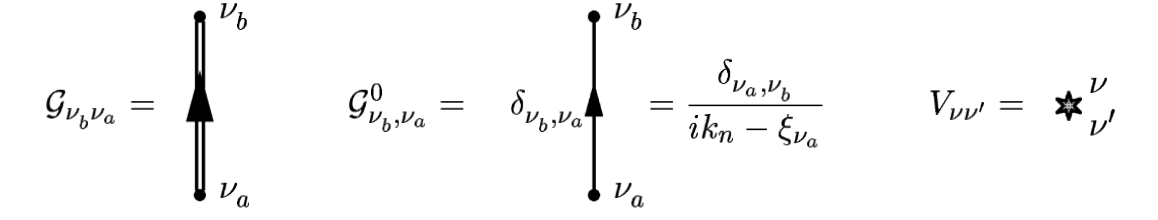
\includegraphics[scale=0.7]{biaoji.png}
  \caption{自能定义}
\end{figure}
戴森方程的图表示为:
\begin{figure}[htbp]
  \centering
  \includegraphics*[scale=0.7]{DaysonEq.png}
  \caption{戴森方程}
\end{figure}
\subsection*{杂质导致的随机势}
现在考虑杂质导致的随机势下的无相互作用电子体系,外场可以写为:
\begin{equation}
  V(\mathbf{r})=\sum_{j=1}^{N_{\mathrm{imp}}} u\left(\mathbf{r}-\mathbf{P}_j\right), \quad \mathbf{P}_j \text { is randomly distributed. }
\end{equation}
在此假设杂质密度远低于电子密度,且u是一个弱且短程的势能\footnote{弱意味着势能远小于能级间隙}。此时戴森展开的第n阶项为:
\begin{equation}
  \begin{aligned}
    \mathcal{G}^{(n)}\left(\mathbf{r}_b, \mathbf{r}_a\right)= & \sum_{j_1}^{N_{\mathrm{imp}}} \ldots \sum_{j_n}^{N_{\mathrm{imp}}} \int d \mathbf{r}_1 \ldots \int d \mathbf{r}_n \\
    & \times \mathcal{G}^0\left(\mathbf{r}_b-\mathbf{r}_n\right) u\left(\mathbf{r}_n-\mathbf{P}_{j_n}\right) \ldots u\left(\mathbf{r}_2-\mathbf{P}_{j_2}\right) \mathcal{G}^0\left(\mathbf{r}_2-\mathbf{r}_1\right) u\left(\mathbf{r}_1-\mathbf{P}_{j_1}\right) \mathcal{G}^0\left(\mathbf{r}_1-\mathbf{r}_a\right)
    \end{aligned}
\end{equation}
严格求解上述方程是没有希望的,但之后可以看到,在取平均以后上述方程有很好的性质。对于方程右式做傅立叶变换,有:
\begin{equation}
  \begin{aligned}
    \mathcal{G}^{(n)}\left(\mathbf{r}_b, \mathbf{r}_a\right)= & \sum_{j_1 \ldots j_n}^{N_{\mathrm{imp}}} \frac{1}{\mathcal{V}^n} \sum_{\mathbf{q}_1 \ldots \mathbf{q}_n} \frac{1}{\mathcal{V}^2} \sum_{\mathbf{k}_a \mathbf{k}_b} \frac{1}{\mathcal{V}^{n-1}} \sum_{\mathbf{k}_1 \ldots \mathbf{k}_{n-1}} \int d \mathbf{r}_1 \ldots \int d \mathbf{r}_n \\
    & \times \mathcal{G}_{\mathbf{k}_b}^0 u_{\mathbf{q}_n} \mathcal{G}_{\mathbf{k}_{n-1}}^0 u_{\mathbf{q}_{n-1}} \ldots u_{\mathbf{q}_2} \mathcal{G}_{\mathbf{k}_1}^0 u_{\mathbf{q}_1} \mathcal{G}_{\mathbf{k}_a}^0 e^{-i\left(\mathbf{q}_n \cdot \mathbf{P}_{j_n}+\ldots+\mathbf{q}_2 \cdot \mathbf{P}_{j_2}+\mathbf{q}_1 \cdot \mathbf{P}_{j_1}\right)} \\
    & \times e^{i \mathbf{k}_b \cdot\left(\mathbf{r}_b-\mathbf{r}_n\right)} e^{i \mathbf{q}_n \cdot \mathbf{r}_n} e^{i \mathbf{k}_{n-1} \cdot\left(\mathbf{r}_n-\mathbf{r}_{n-1}\right)} \ldots e^{i \mathbf{q}_2 \cdot \mathbf{r}_2} e^{i \mathbf{k}_1 \cdot\left(\mathbf{r}_2-\mathbf{r}_1\right)} e^{i \mathbf{q}_1 \cdot \mathbf{r}_1} e^{i \mathbf{k}_a \cdot\left(\mathbf{r}_1-\mathbf{r}_a\right)}
    \end{aligned}
\end{equation}
利用空间积分给出的delta函数,再对左式也做傅立叶变换,可以化简为:
\begin{equation}
  \begin{aligned}
    \mathcal{G}_{\mathbf{k}_b \mathbf{k}_a}^{(n)}= & \sum_{j_1 \ldots j_n}^{N_{\text {imp }}} \frac{1}{\mathcal{V}^{n-1}} \sum_{\mathbf{k}_1 \ldots \mathbf{k}_{n-1}} e^{-i\left[\left(\mathbf{k}_b-\mathbf{k}_{n-1}\right) \cdot \mathbf{P}_{j_n}+\ldots+\left(\mathbf{k}_1-\mathbf{k}_a\right) \cdot \mathbf{P}_{j_1}\right]} \\
    & \times \mathcal{G}_{\mathbf{k}_b}^0 u_{\mathbf{k}_b-\mathbf{k}_{n-1}} \mathcal{G}_{\mathbf{k}_{n-1}}^0 \cdots u_{\mathbf{k}_2-\mathbf{k}_1} \mathcal{G}_{\mathbf{k}_1}^0 \cdots u_{\mathbf{k}_1-\mathbf{k}_a} \mathcal{G}_{\mathbf{k}_a}^0 .
    \end{aligned}
\end{equation}
可以看出,动量为k的粒子每次被散射以后动量都将发生改变,在引入新的假设前这无法被化简。
\subsection*{杂质自平均}
当温度升高时,电子与电子、声子、杂质之间的散射事件增加,每次散射都将使得电子波函数的相位发生变化,因此电子间的关联长度随着温度升高而减小。当样品远大于相关长度时,对于物理量的测量就是对于不同相关长度大小的小区域分别测量并求平均。对杂质场的求平均数学上需要对N个辅助体系都算出来再求平均,某些情况下等价于对杂质位置求平均:
\begin{equation}
  \frac{1}{\mathcal{V}}\left\langle\mathcal{G}_{\mathbf{k}_b \mathbf{k}_a}\right\rangle_{\mathrm{imp}} \equiv \delta_{\mathbf{k}_b, \mathbf{k}_a} \overline{\mathcal{G}}_{\mathbf{k}_a} \equiv \frac{\delta_{\mathbf{k}_b, \mathbf{k}_a}}{N_{\mathrm{sys}}} \sum_{i=1}^{N_{\mathrm{sys}}} \mathcal{G}_{\mathbf{k}_a}^{\mathrm{sys}_{\mathrm{i}}} \sim \delta_{\mathbf{k}_b, \mathbf{k}_a} \frac{1}{\mathcal{V}} \int d \mathbf{P}_1 \frac{1}{\mathcal{V}} \int d \mathbf{P}_2 \cdots \frac{1}{\mathcal{V}} \int d \mathbf{P}_{N_{\mathrm{imp}}} \mathcal{G}_{\mathbf{k}_a}
\end{equation}
需要注意到,戴森级数中的第n项包含n次散射,但其中的一些散射过程可能发生在同一点。由于假设杂质密度低,对于一个杂质的散射为Leading oder,其次是两个杂质的散射。由此
将求和拆解:
\begin{equation}
  \begin{aligned}
    & \sum_{j_1, \ldots, j_n}^{N_{\mathrm{imp}}} e^{i \sum_{l=1}^n \mathbf{q}_l \cdot \mathbf{P}_{j_l}}=\sum_{h_1}^{N_{\mathrm{imp}}} e^{i\left(\sum_{\mathbf{q}_{j_1} \in Q} \mathbf{q}_{j_1}\right) \cdot \mathbf{P}_{h_1}} \\
    & +\sum_{Q_1 \cup Q_2=Q} \sum_{h_1}^{N_{\mathrm{imp}}} \sum_{h_2}^{N_{\mathrm{imp}}} e^{i\left(\sum_{\mathbf{q}_{l_1} \in Q_1} \mathbf{q}_{l_1}\right) \cdot \mathbf{P}_{h_1}} e^{i\left(\sum_{\mathbf{q}_{l_2} \in Q_2} \mathbf{q}_{l_2}\right) \cdot \mathbf{P}_{h_2}} \\
    & +\sum_{Q_1 \cup Q_2 \cup Q_3=Q} \sum_{h_1}^{N_{\mathrm{imp}}} \sum_{h_2}^{N_{\mathrm{imp}}} \sum_{h_3}^{N_{\mathrm{imp}}} e^{i\left(\sum_{\mathbf{q}_{l_1} \in Q_1} \mathbf{q}_{l_1}\right) \cdot \mathbf{P}_{h_1}} e^{i\left(\sum_{\mathbf{q}_{l_2} \in Q_2} \mathbf{q}_{l_2}\right) \cdot \mathbf{P}_{h_2}} e^{i\left(\sum_{\mathbf{q}_{l_3} \in Q_3} \mathbf{q}_{l_3}\right) \cdot \mathbf{P}_{h_h}}\\
    & +\ldots
    \end{aligned}
\end{equation}
其中$ Q=\left\{\mathbf{q}_1, \mathbf{q}_2, \ldots, \mathbf{q}_n\right\} $为n个散射波矢。所有在同一子集$ Q_i $中的波矢都被同一杂质散射。\footnote{严格来说同一点中不能有多个杂质,上述求和之间相互没有限制,会引入$ 1 / N_{\mathrm{imp}} $阶的误差 }\\

可以预想到,在求平均以后,平移不变性恢复,对同一点杂质的散射动量守恒。每个指数因子的平均给出一个delta函数:
\begin{equation}
  \left\langle e^{i\left(\sum_{\mathbf{q}_{h_i} \in Q_i} \mathbf{q}_{h_i}\right) \cdot \mathbf{P}_{h_i}}\right\rangle_{\mathrm{imp}}=\frac{1}{\mathcal{V}} \int d \mathbf{P}_{h_i} e^{i\left(\sum_{\mathbf{q}_{h_i} \in Q_h} \mathbf{q}_{h_i}\right) \cdot \mathbf{P}_{h_i}}=\delta_{0, \sum_{\mathbf{q}_{h_i} \in Q_h} \mathbf{q}_{h_i}} .
\end{equation}
对于n阶戴森级数展开的平均有:
\begin{equation}
  \begin{aligned}
    \left\langle\mathcal{G}_{\mathbf{k}}^{(n)}\right\rangle_{\mathrm{imp}}= & \frac{1}{\mathcal{V}^{n-1}} \sum_{\mathbf{k}_1 \ldots \mathbf{k}_{n-1}} \sum_{p=1}^n \sum_{\bigcup_{h=1}^p Q_h=Q} \prod_{h=1}^p\left(N_{\mathrm{imp}} \delta_{0, \Sigma_{Q_h}\left(\mathbf{k}_{h_i}-\mathbf{k}_{\left(h_i-1\right)}\right)}\right) \\
    & \times \mathcal{G}_{\mathbf{k}}^0 u_{\mathbf{k}-\mathbf{k}_1} \mathcal{G}_{\mathbf{k}_1}^0 u_{\mathbf{k}_1-\mathbf{k}_2} \mathcal{G}_{\mathbf{k}_2}^0 \ldots u_{\mathbf{k}_{n-1}-\mathbf{k}} \mathcal{G}_{\mathbf{k}}^0 .
    \end{aligned}
\end{equation}
由于每个杂质给出一个delta函数,因此还剩下n-1-p个动量求和,剩下的p个体积倒数同$ N_{imp} $组成杂质密度,因此图中每个杂质贡献一个杂质密度。
\subsection*{被杂质散射的电子的自能}
自能定义为传播子中的所有单粒子不可约图的求和,并去掉两端的格林函数。
\begin{figure}[htbp]
  \centering
  \includegraphics*[scale=0.7]{selfenergy.png}
  \caption{<caption>}
  \label{<label>}
\end{figure}
通过形式上的等比级数求和,可以将完整格林函数用裸格林函数与自能表示出:
\begin{equation}
  \left\langle\mathcal{G}_{\mathbf{k}}\left(i k_n\right)\right\rangle_{\mathrm{imp}}=\frac{\mathcal{G}_{\mathbf{k}}^0}{1-\mathcal{G}_{\mathbf{k}}^0 \Sigma_{\mathbf{k}}}=\frac{1}{\left(\mathcal{G}_{\mathbf{k}}^0\right)^{-1}-\Sigma_{\mathbf{k}}}=\frac{1}{i k_n-\xi_{\mathbf{k}}-\Sigma_{\mathbf{k}}\left(i k_n\right)}
\end{equation}
求解格林函数的问题现在转换为求解自能,下面对自能进行逐级近似。\\

最低阶的近似是只考虑单点、单次的散射过程:$ \Sigma_{\mathbf{k}}^{\mathrm{LOA}}\left(i k_n\right) \equiv n_{\mathrm{imp}} u_0=n_{\mathrm{imp}} \int d \mathbf{r} u(\mathbf{r}), $,这只是将激发的能量平移了一个常数,可以通过平移化学势使得这种项没有贡献。
\subsection*{一阶玻恩近似}
现在自能图只考虑单个杂质散射两次\footnote{模方来自u(r)是个实函数,它的傅立叶变换正负部分互为共轭}:
\begin{equation}
  \Sigma_{\mathbf{k}}^{1 \mathrm{BA}}\left(i k_n\right) \equiv n_{\mathrm{imp}} \sum_{\mathbf{k}^{\prime}}\left|u_{\mathbf{k}-\mathbf{k}^{\prime}}\right|^2 \frac{1}{i k_n-\xi_{\mathbf{k}^{\prime}}}
\end{equation}
此时的自能是个复数,这使得完全格林函数的极点从实轴上移到复平面上,由此具有有限寿命。将自能的自变量延拓到实轴,有\footnote{其中用到了delta函数的另一种形式:$ \delta(x)=\lim _{\varepsilon \rightarrow 0} \frac{1}{\pi} \frac{\varepsilon}{\varepsilon^2+x^2} . $ }:
\begin{equation}
  \begin{aligned}
    \Sigma_{\mathbf{k}}^{1 \mathrm{BA}}\left(\omega+i \operatorname{sgn}\left(k_n\right) \eta\right) & =n_{\mathrm{imp}} \sum_{\mathbf{k}^{\prime}}\left|u_{\mathbf{k}-\mathbf{k}^{\prime}}\right|^2 \frac{1}{\left(\omega-\xi_{\mathbf{k}^{\prime}}\right)+i \operatorname{sgn}\left(k_n\right) \eta} \\
    & =\sum_{\mathbf{k}^{\prime}} n_{\mathrm{imp}}\left|u_{\mathbf{k}-\mathbf{k}^{\prime}}\right|^2\left[\frac{\omega-\xi_{\mathbf{k}^{\prime}}}{\left(\omega-\xi_{\mathbf{k}^{\prime}}\right)^2+\eta^2}-i \operatorname{sgn}\left(k_n\right) \pi \delta\left(\omega-\xi_{\mathbf{k}^{\prime}}\right)\right] .
    \end{aligned}
\end{equation}
由于考虑的情况中温度总是远小于费米能,我们关注费米面附近的激发,即考虑如下范围:
\begin{equation}
  |\mathbf{k}| \sim k_{\mathrm{F}} \quad \text { and } \quad\left|i k_n \rightarrow \omega+i \operatorname{sgn}\left(k_n\right) \eta\right| \ll \varepsilon_{\mathrm{F}} .
\end{equation}
由于电子的重分布将屏蔽杂质带来的额外电荷,$ u_k $可以看作一个上述区间内变化较慢的函数,可以得到,自能的实部趋近于零,剩下一个虚部:
\begin{equation}
  \Sigma_{\mathbf{k}}^{1 \mathrm{BA}}\left(i k_n\right)=-i \pi \operatorname{sgn}\left(k_n\right) \sum_{\mathbf{k}^{\prime}} n_{\text {imp }}\left|u_{\mathbf{k}-\mathbf{k}^{\prime}}\right|^2 \delta\left(\xi_{\mathbf{k}}-\xi_{\mathbf{k}^{\prime}}\right)=-i \operatorname{sgn}\left(k_n\right) \frac{1}{2 \tau_{\mathbf{k}}},
\end{equation} 
上面引入了杂质散射时间:$ \frac{1}{\tau_{\mathbf{k}}} \equiv 2 \pi \sum_{\mathbf{k}^{\prime}} n_{\mathrm{imp}}\left|u_{\mathbf{k}-\mathbf{k}^{\prime}}\right|^2 \delta\left(\xi_{\mathbf{k}}-\xi_{\mathbf{k}^{\prime}}\right) $。由此可以得到完全格林函数,并延拓到复平面:
\begin{equation}
  \mathcal{G}_{\mathbf{k}}^{1 \mathrm{BA}}\left(i k_n\right)=\frac{1}{i k_n-\xi_{\mathbf{k}}+i \frac{\operatorname{sgn}\left(k_n\right)}{2 \tau_{\mathbf{k}}}} \underset{i k_n \rightarrow z}{\longrightarrow} \mathcal{G}_{\mathbf{k}}^{1 \mathrm{BA}}(z)=\left\{\begin{array}{l}
    \frac{1}{z-\xi_{\mathbf{k}}+\frac{i}{2 \tau_{\mathbf{k}}}}, \operatorname{Im} z>0 \\
    \frac{1}{z-\xi_{\mathbf{k}}-\frac{i}{2 \tau_{\mathbf{k}}}}, \operatorname{Im} z<0 .
    \end{array}\right.	
\end{equation} 
计算时域以及位置空间的格林函数可以看到,一阶玻恩近似的自能项中包含的虚部,使得传播子在时间和空间上都指数衰减。
\subsection*{完全玻恩近似}
完全玻恩近似是指考虑含有一个杂质散射的所有图,这在$ n_{imp} $阶是完全的,此时自能的图表示为:
\begin{figure}[htbp]
  \centering
  \includegraphics*[scale=0.7]{FBASE.png}
  \caption{完全玻恩近似的自能图表示}
\end{figure} 
引入转移矩阵,图表示为:
\begin{figure}[htbp]
  \centering
  \includegraphics*[scale=0.7]{tmatrix.png}
  \caption{t矩阵的图表示}
\end{figure}
可以看出自能就是t矩阵的对角元。仍只考虑费米面附近的电子,此时t矩阵的实部近似为常数,可以被重定义化学式抵消,而虚部可以利用光学定理\footnote{由图表示可得到矩阵方程:$ t=u+u \mathcal{G}^0 t $。由于u是厄米矩阵,同时求厄米共轭再代回有:$ t=u+\left(t^{\dagger} \mathcal{G}^0 t-t^{\dagger}\left(\mathcal{G}^0\right)^{\dagger} u \mathcal{G}^0 t\right) $,只有中间
一项是非厄米的,因此虚部全部来自于它:$ \operatorname{Im} t_{\mathbf{k}, \mathbf{k}}=\operatorname{Im}\left\langle\mathbf{k}\left|t^{\dagger} \mathcal{G}^0 t\right| \mathbf{k}\right\rangle=\operatorname{Im} \sum_{\mathbf{k}^{\prime}} t_{\mathbf{k}, \mathbf{k}^{\prime}}^{\dagger} \mathcal{G}_{\mathbf{k}^{\prime}}^0 t_{\mathbf{k}^{\prime}, \mathbf{k}} $   }:
\begin{equation}
  \begin{aligned}
    & \operatorname{Im} \Sigma_{\mathbf{k}}^{\mathrm{FBA}}\left(i k_n\right)= \operatorname{Im} t_{\mathbf{k}, \mathbf{k}}\left(i k_n\right)=\operatorname{Im} \sum_{\mathbf{k}^{\prime}} \frac{\left|t_{\mathbf{k}, \mathbf{k}^{\prime}}\right|^2}{i k_n-\xi_{\mathbf{k}^{\prime}}} \\
    & \underset{i k_n \rightarrow \omega+i \operatorname{sgn}\left(k_n\right) \eta}{\longrightarrow}-\operatorname{sgn}\left(k_n\right) \pi \sum_{\mathbf{k}^{\prime}}\left|t_{\mathbf{k}, \mathbf{k}^{\prime}}\right|^2 \delta\left(\omega-\xi_{\mathbf{k}^{\prime}}\right) .
    \end{aligned}
  \label{fba}
\end{equation}
可以看到,它和一阶玻恩近似的虚部长的差不多,只不过$ n_{\mathrm{imp}}\left|u_{\mathbf{k}-\mathbf{k}^{\prime}}\right|^2\to\left|t_{\mathbf{k}, \mathbf{k}^{\prime}}\right|^2 $。
\subsection*{自洽玻恩近似} 
通过将裸传播子换位全传播子,可得到一个自洽方程,若仍只考虑单杂质散射,就是自洽玻恩近似,此时的自能或者是转移矩阵的对角元为:
\begin{equation}
  t_{\mathbf{k}}^{\mathrm{SCBA}} \equiv n_{\mathrm{imp}}\left[u_0 \delta_{\mathbf{k}, \mathbf{k}}+\sum_{\mathbf{k}^{\prime}} u_{\mathbf{k}-\mathbf{k}^{\prime}} \mathcal{G}_{\mathbf{k}^{\prime}} t_{\mathbf{k}^{\prime}, \mathbf{k}}\right]
\end{equation}
由于相同的论述,实部可以略去,关注虚部:
\begin{equation}
  \Sigma_{\mathbf{k}}^i=\operatorname{Im} \sum_{\mathbf{k}^{\prime}} \frac{\left|t_{\mathbf{k}, \mathbf{k}^{\prime}}^{\mathrm{SCBA}}\right|^2}{i k_n-\xi_{\mathbf{k}^{\prime}}-i \Sigma_{\mathbf{k}^{\prime}}^i}
\end{equation}
它与\eqref{fba}不同点在于使用的是上述自洽方程给出的转移矩阵。最终求和的图中不包括带交叉的图,因为我们总考虑费米面附近的动量,带交叉的图积分的动量空间总比不带交叉的图小。
\subsection*{一些评注}
这一节内容中总是强调费米面附近,以及最终的不考虑交叉图的结论,在此做出一些解释。Dayson级数的迭代中总使用裸传播子:$ G_p \equiv \frac{1}{-i \omega_n+\frac{\mathbf{p}^2}{2 m}-\mu} $,化学势可与费米能近似,因此
裸传播子的值总是在费米动能处很大,对积分也主要是费米球附近的薄球壳贡献。在比较交叉图与非交叉图的贡献时,要求裸传播子的动量在球壳上。内线的动量会被积分,交叉图的积分动量空间总是比同阶的非交叉图小很多,因此贡献忽略。随机相位
近似也是这个道理。
\section{Introduction to SYK model}
\subsection{Random Matrix theory}
SYK model is a model of four fermions with random coupling, before going to this, let's briefly introduce a simpler version, which is a two fermions with random hopping term, namely random matrix theory.\\
The Hamiltonian for random matrix theory is given by
\begin{equation}
  H_2=\frac{1}{(N)^{1 / 2}} \sum_{i, j=1}^N t_{i j} c_i^{\dagger} c_j-\mu \sum_i c_i^{\dagger} c_i
\end{equation}
$c_i$ are complex fermion and the summation to N is taken to the limit $ N\to\infty $. The hopping matrix elements, $ t_{ij} $ are random complex numbers satisfying $\overline{t_{i j}}=0$ and $ \overline{\left|t_{i j}\right|^2}=t^2 $. As usual, we want to solve this problem perturbatively, starting from the "non-interacting" Green Function
\begin{equation*}
  G_{i j}^0\left(i \omega_n\right)=\frac{\delta_{i j}}{i \omega_n+\mu}
\end{equation*}
And then using Dyson's equation to get the full Green function, then the problem turn to be finding the self-energy, which seems to be complicated, but is simplified here for the large N limit and random hopping matrix. The only OPI diagram remains that will contribute to the self-energy is:
\begin{figure}[h]
  \centering
  \includegraphics*[scale = 1]{Figures/RMT.png}
  \caption{The only OPI diagram contributes to the self-energy}
  \label{RMT}
\end{figure}
It's easy to write this term using Feynman rule, and combined with Dyson's equation, we get
\begin{equation}
  \begin{aligned}
    G\left(i \omega_n\right) & =\frac{1}{i \omega_n+\mu-\Delta\left(i \omega_n\right)}, \\
    \Delta(\tau) & =t^2 G(\tau),
    \end{aligned}
\end{equation}
It's just a quadratic equation for $ G(z) $, thus the solution for complex frequency is
\begin{equation}
  G(z)=\frac{1}{2 t^2}\left(z+\mu \pm \sqrt{(z+\mu)^2-4 t^2}\right)
\end{equation} 
\section{SYK model}
SYK model is a four fermions with random coupling, the Hamiltonian is given by
\begin{equation}
  H_4=\frac{1}{(2 N)^{3 / 2}} \sum_{i j k \ell=1}^N U_{i j ; k \ell} c_i^{\dagger} c_j^{\dagger} c_k c_{\ell}-\mu \sum_i c_i^{\dagger} c_i
\end{equation}
\indent The coupling elements satisfying $ \overline{U_{i j ; k \ell}}=0 $ and $ \mid \overline{\left|U_{i j ; k \ell}\right|^2}=U^2 $. Similar results can be obtained as the random matrix theory: the only diagram survive in the large N limit and average over random coupling is the following melon diagram
\begin{figure}[!h]
  \centering
  \includegraphics*[scale = 0.5]{Figures/melon.png}
  \caption{The melon diagram}
  \label{melon}
\end{figure}
\indent The term for this diagram and the Dyson's equation combined to give
\begin{equation}
  G\left(i \omega_n\right)=\frac{1}{i \omega_n+\mu-\Sigma\left(i \omega_n\right)}
  \label{dyson}
\end{equation}
\begin{equation}
  \Sigma(\tau)=-U^2 G^2(\tau) G(-\tau)
  \label{selfenergy}
\end{equation}
\indent Simple as the equation looks like, it's much harder to solve compare to the random matrix case due to the fact that it's both non-linear and integral. But as a physicist we can always guess the solution.\\
\indent The first solution one may have a try is a solution with gap $ \Delta $, which means the spectral function defined as $ \rho(\omega) = -2\Im G(\omega+i\delta) = 0, \omega<\Delta$, and this gives a exponentially decaying green function in time domain with "correlation time" $ \frac{1}{\Delta} $, then \eqref{selfenergy} gives that the self-energy would have a "correlation time" $ \frac{1}{3\Delta} $, thus the imaginary part of the self-energy in frequency domain would have a gap of $ 3\Delta $, which would lead to a contradiction of gap in \eqref{dyson}, so the self-consistency constraints that the solution must be gapless.
\subsection{Solution to SYK model}

\indent A natural guess for the Green function of a gapless system is power law decay in the low energy region, so an ansatz for Green function in complex frequency domain would be
\begin{equation}
  G(z)=C \frac{e^{-i(\pi \Delta+\theta)}}{z^{1-2 \Delta}}, \quad \operatorname{Im}(z)>0, \quad|z| \ll U
  \label{ansatz}
\end{equation}
$ \theta $ is the parameter which characterizes the asymmetry between particle and hole, since here we always focus on half-filling, it's not important for our discussion, but it should be mentioned that the value of $ \theta $ is determined by the filling fraction $ \mathcal{Q} $ with a generalized Luttinger's theorem.\\
Having this ansatz solution, turn to the time domain using Fourier transform, one have
\begin{equation*}
  G(\tau)\sim \frac{1}{\tau^{2\Delta}} \text{for} \ \tau \gg \frac{1}{U}
\end{equation*}
plug in to \eqref{dyson}, the self-energy would have scale as $ \Sigma(\tau)\sim\frac{1}{\Delta^{6}} $, and turn back to frequency domain $\Sigma(z)\sim z^{6\Delta-1}$.\\
\indent By comparing the divergence when $ z\to 0 $ in \eqref{dyson}, the self-consistency would demand
\begin{equation}
  \begin{aligned}
    \mu-\Sigma(0) & =0 \\
    1-2 \Delta & =6 \Delta-1 \Rightarrow \Delta=\frac{1}{4}
    \end{aligned}
\end{equation}
thus indeed we would have a solution of Green function which decay as $ 1/\sqrt{\tau} $, and this solution would have many implications.
\subsection{No quasiparticle}
 The power law decay Green function in frequency domain suggest that the system has no quasiparticle particle excitation, since there is no delta function term. However, this is a crude statement, no delta function only means the excitation doesn't looks like free fermion excitation.\\
 \indent A more rigorous way to define no quasiparticle excitation is to look at the many-body density of states. The low energy excitation for a system with quasiparticle will be the addition of quasiparticle, thus the density of states' spacing scales $ \frac{1}{N} $ as the system size, much smaller than a system without quasiparticle, which scales exponentially as $ \exp^{-N} $.
\subsection{Time Reparameterization And Gauge Symmetry}
The \eqref{dyson} can be simplified if we make the assumption, which will turn out to be correct, that in the low energy limit, the denominator is dominated by the singular part of the self energy $ \Sigma_{\text{sing}} $, and the equation will become
\begin{equation*}
  \begin{array}{r}
    \int_0^\beta d \tau_2 \Sigma_{\text {sing }}\left(\tau_1, \tau_2\right) G\left(\tau_2, \tau_3\right)=-\delta\left(\tau_1-\tau_3\right) \\
    \Sigma_{\text {sing }}\left(\tau_1, \tau_2\right)=-U^2 G^2\left(\tau_1, \tau_2\right) G\left(\tau_2, \tau_1\right)
    \end{array}
\end{equation*}
\indent We have turn to the bilocal form, which is natural in the path integral formalism, and keep in mind that the true solution only depend on the difference of time. One can check that these equations have the following symmetry,  
\begin{equation*}
  \begin{aligned}
    \tau & =f(\sigma), \\
    G\left(\tau_1, \tau_2\right) & =\left[f^{\prime}\left(\sigma_1\right) f^{\prime}\left(\sigma_2\right)\right]^{-1 / 4} \frac{g\left(\sigma_1\right)}{g\left(\sigma_2\right)} \tilde{G}\left(\sigma_1, \sigma_2\right), \\
    \Sigma\left(\tau_1, \tau_2\right) & =\left[f^{\prime}\left(\sigma_1\right) f^{\prime}\left(\sigma_2\right)\right]^{-3 / 4} \frac{g\left(\sigma_1\right)}{g\left(\sigma_2\right)} \tilde{\Sigma}\left(\sigma_1, \sigma_2\right),
    \end{aligned}
\end{equation*} 
and by choosing $ \tau=\frac{1}{\pi T} \tan (\pi T \sigma) $ one can get the solution to SYK model in finite temperature
\begin{equation*}
  G(\tau)=B \operatorname{sgn}(\tau)\left|\frac{\pi T}{\sin (\pi T \tau)}\right|^{1 / 2}, \quad T,|\tau|^{-1} \ll U
\end{equation*}
\indent However, the true solution is only a function of time difference, thus the symmetry is broken, the reparametrization will be constraint by requiring that if $ G\left(\tau_1, \tau_2\right)=G_c\left(\tau_1-\tau_2\right) $, then $ \tilde{G}\left(\sigma_1, \sigma_2\right)=G_c\left(\sigma_1-\sigma_2\right) $, and the reparametrization satisfying this would form a group of $ \operatorname{SL}(2, \mathrm{R}) $,
\begin{equation*}
  f(\tau)=\frac{a \tau+b}{c \tau+d}, \quad a d-b c=1
\end{equation*}     
which is isomorphic to the symmetry of $ \mathrm{AdS}_2 $ metric.


\section{Peierls相变}
一维完美的格点是不稳定的,总会发生二聚化形成绝缘体,这称为Peierls相变。对于晶格间距为a的一维格点,紧束缚模型给出能带:
\begin{equation}
	\varepsilon_1(k)=-t\left[e^{i k a}+e^{-i k a}\right]=-2 t \cos (k a)
\end{equation}
假设发生二聚化,跃迁系数可以近似为:$ t^{\prime}(a \pm 2 b) \approx t \pm 2 b * \frac{\mathrm{d} t}{\mathrm{~d} a}=t \pm b * q_0=t \mp \Delta $,此时紧束缚模型给出两条能带:
\begin{equation}
	\begin{aligned}
		& H_2= {\left[\begin{array}{cc}
		0 & (t+\Delta)+(t-\Delta) \cdot e^{-i 2 k a} \\
		(t+\Delta)+(t-\Delta) \cdot e^{i 2 k a}
		\end{array}\right] } \\
		&= {\left[\begin{array}{cc}
		0 & 2 e^{-i k a}[t \cos (k a)+i \Delta \sin (k a)] \\
		2 e^{i k a}[t \cos (k a)-i \Delta \sin (k a)]
		\end{array}\right] } \\
		& \Rightarrow \quad \varepsilon_2(k)= \pm 2 \sqrt{t^2 \cos ^2(k a)+\Delta^2 \sin ^2(k a)}
		\end{aligned}
\end{equation} 
此时能带具有能隙。再考虑二聚化使得院子之间的能量发生的变换,一维声子的色散关系为:
\begin{equation}
	\omega=\sqrt{\frac{4 K}{M}}\left|\sin \frac{q a}{2}\right|
\end{equation}
二聚化相当于一个波矢为$ \frac{\pi}{a} $,振幅为b的格波,对应的能量为:
\begin{equation}
	\begin{aligned}
		\Delta E_{\ell} & =N \cdot \frac{1}{2} M \omega_{q=\frac{\pi}{a}}^2 b^2 \\
		& =N \cdot 2 K b^2
		\end{aligned}
\end{equation} 
由于能隙打开使得电子的能量改变量为:
\begin{equation}
	\begin{aligned}
		\Delta E_e & =\frac{N a}{2 \pi} \int_{-\pi / 2 a}^{\pi / 2 a}\left[\varepsilon_2(k)-\varepsilon_1(k)\right] \mathrm{d} k \\
		& =-2 t \frac{N a}{2 \pi} \int_{-\pi / 2 a}^{\pi / 2 a}\left[\sqrt{\cos ^2(k a)+\frac{\Delta^2}{t^2} \sin ^2(k a)}-\cos (k a)\right] \mathrm{d} k \\
		& =-2 t \frac{N}{\pi} \int_0^{\pi / 2}\left[\sqrt{\cos ^2(\theta)+\frac{\Delta^2}{t^2} \sin ^2(\theta)}-\cos (\theta)\right] \mathrm{d} \theta \\
		& =-2 t \frac{N}{\pi} \int_0^{\pi / 2}\left[\sqrt{\cos ^2(\theta)+\frac{\Delta^2}{t^2} \sin ^2(\theta)}-\cos (\theta)\right] \mathrm{d} \theta \\
		& =-2 t \frac{N}{\pi}\left[\int_0^{\pi / 2} \sqrt{1-(1-\lambda) \sin ^2(\theta)} \mathrm{d} \theta-1\right]
		\end{aligned}
\end{equation}
此积分对于$ \lambda $很小时可以近似给出:$ E(1-\lambda)=1+\lambda\left[a_1-\frac{1}{4} \ln (\lambda)\right]+\mathcal{O}\left(\lambda^2\right), \quad a_1=0.463 $,总能量的改变为声子与电子两部分的和:  
\begin{equation}
	\begin{aligned}
		&\begin{aligned}
		\Delta E_t & =\Delta E_{\ell}+\Delta E_e \\
		& =N \lambda[\alpha+\beta \ln \lambda]
		\end{aligned}\\
		&\alpha=\frac{2 K t^2}{q_0^2}-\frac{a_1 t}{\pi}, \quad \beta=\frac{t}{\pi}
		\end{aligned}
\end{equation}
稳定的构型对应的b由能量极值给出:$ \frac{\mathrm{d} \Delta E_t}{\mathrm{~d} \lambda}=0 $,则有:
\begin{equation}
	\begin{aligned}
		& \ln \lambda=-\frac{\alpha+\beta}{\beta} \\
		& \Delta E_t=N \beta \exp \left(-\frac{\alpha+\beta}{\beta}\right)
		\end{aligned}
\end{equation} 
可以看出只要$ \beta>0 $,对任意的$ \alpha,\beta $二聚化总是使得能量下降。  

\section{Quantum-Classical Correspondence}
\section{Wick定理的多种形式}
\subsection{凝聚态与QFT中的Wick定理}
\subsection{统计中的“wick”定理}
\section{Hartree-Fock近似}
Hartree-Fock的本质是用无相互作用基态作为试探解,此时我们仍旧有占据数的物理图像。利用能量最小的变分原理求得占据数$ n_{\vec{k},\alpha} $。\href{https://www.zhihu.com/question/29462902/answer/2967943520}{怎样理解 Hartree-Fock Method? - O空O扬O的回答 - 知乎}
\subsection{基态能量}
考虑一个一般的两体相互作用动量空间的哈密顿量:
\begin{equation}
  H=\sum_{\mathbf{k}} \xi_{\mathbf{k}} c_{\alpha \mathbf{k}}^{\dagger} c_{\alpha \mathbf{k}}+\frac{1}{2 N_{s i t e}} \sum_{\mathbf{k}, \mathbf{k}^{\prime}, \mathbf{q}} c_{\alpha \mathbf{k}}^{\dagger} c_{\alpha, \mathbf{k}-\mathbf{q}} V_{\mathbf{q}} c_{\beta, \mathbf{k}^{\prime}}^{\dagger} c_{\beta, \mathbf{k}^{\prime}+\mathbf{q}}
\end{equation}
利用无相互作用的的基态$ \left|\Psi_0\right\rangle $作为试探解,它完全由占据数描述,对于此态,能量期望值为:
\begin{equation}
  \begin{aligned}
    \left\langle\Psi_0|H| \Psi_0\right\rangle= & \left\langle\Psi_0\left|H_0\right| \Psi_0\right\rangle+\frac{1}{2} \sum_{\mathbf{i}, \mathbf{j}}\left\langle c_\alpha^{\dagger}(\mathbf{i}) c_\alpha(\mathbf{i})\right\rangle V(\mathbf{i}-\mathbf{j})\left\langle c_\beta^{\dagger}(\mathbf{j}) c_\beta(\mathbf{j})\right\rangle \\
    & +\frac{1}{2} \sum_{\mathbf{i}, \mathbf{j}}\left\langle c_\alpha^{\dagger}(\mathbf{i}) c_\beta(\mathbf{j})\right\rangle V(\mathbf{i}-\mathbf{j})\left\langle c_\alpha(\mathbf{i}) c_\beta^{\dagger}(\mathbf{j})\right\rangle
    \end{aligned}
\end{equation} 
第一项为动能,第二项为Hatree项,可改写为:$ \frac{1}{2} \sum_{i, j} \rho(i) V(i-j) \rho(j) $,代表经典势能。 它们都与自旋比例无关。
第三项为Fock项,可改写为:
\begin{equation*}
  \frac{1}{2 N_s} \sum_{\mathbf{k}, \mathbf{k}^{\prime}, \mathbf{q}} V_{\mathbf{q}}\left\langle c_{\mathbf{\alpha k}}^{\dagger} c_{\beta \mathbf{k}^{\prime}+\mathbf{q}}\right\rangle\left\langle c_{\alpha \mathbf{k}-\mathbf{q}} c_{\beta \mathbf{k}^{\prime}}^{\dagger}\right\rangle=-\frac{1}{2 N_s} \sum_{\mathbf{k , \mathbf { q } , \mathbf { \alpha }}} V_{\mathbf{q}} n_{\mathbf{k}, \mathbf{\alpha}} n_{\mathbf{k}-\mathbf{q}, \alpha}+\frac{1}{2} V(0) N
\end{equation*}
它代表相同自旋的有效吸引,修正了Hatree项对于相同自旋相互作用过高的估计。试探态的总能量为:
\begin{equation}
  \begin{aligned}
    & \left\langle\Psi_{\left\{n_{\mathbf{k}, \alpha}\right\}}|H| \Psi_{\left\{n_{\mathbf{k}, \alpha}\right\}}\right\rangle \\
    = & \sum_{\mathbf{k}, \alpha} n_{\mathbf{k}, \alpha}\left(\epsilon_{\mathbf{k}}-\mu+\frac{V_0}{2}\right)+\frac{V_0}{2 N_s}\left(\sum_{\mathbf{k}, \alpha} n_{\mathbf{k}, \alpha}\right)^2-\frac{1}{N_s} \sum_{\mathbf{k}, \mathbf{q}, \alpha} \frac{V_{\mathbf{q}}}{2} n_{\mathbf{k}, \alpha} n_{\mathbf{k}-\mathbf{q}, \alpha}
    \end{aligned}
\end{equation}
经过简单的线性变分,可以得到占据数:
\begin{equation}
  \begin{aligned}
    & n_{\mathbf{k}, \alpha}=1, \quad \epsilon_{\mathbf{k}}-\mu^{\prime}+\sum_{\mathbf{k}, \mathbf{\alpha}}<0 \\
    & n_{\mathbf{k}, \alpha}=0, \quad \epsilon_{\mathbf{k}}-\mu^{\prime}+\sum_{\mathbf{k}, \alpha}>0 \\
    &
    \end{aligned}
\end{equation}
其中$ \sum_{\mathbf{k}, \alpha}=-\frac{1}{N_s} \sum_{\mathbf{k}, \alpha} V_{\mathbf{q}} n_{\mathbf{k}-\mathbf{q}, \alpha} $,$ \mu^{\prime}=\mu-\rho_0 V_0-\frac{1}{2} V(0) $。
这给出了占据数的隐函数解。这也可以看作一个自洽性条件:我们已经预设了基态是某个零温自由费米子的基态,上述方程给出了费米动量的自洽条件。上面的$ \sum_{\mathbf{k}, \alpha} $本身按照定义是对k的求和,是q的函数,但为了方便又将
之后的求和哑指标q换为k,因此它最后是k的函数。 

\subsection{激发谱} 
现在考虑基态之上的激发,也取基态激发的波函数为无相互作用的波函数,由占据数$ n_{\mathbf{k}, \alpha}+\delta n_{\mathbf{k}, \alpha} $刻画。激发能量为:
\begin{equation}
  \delta E=\sum_{\mathbf{k}, \alpha} \delta n_{\mathbf{k}, \alpha}\left(\epsilon_{\mathbf{k}}-\mu^{\prime}+\sum_{\mathbf{k}, \alpha}\right)
\end{equation} 
可以做出总结,在Hatree-Fock近似下,相互作用系统的低能激发由一个自由费米系统描述,特别的:
\begin{itemize}
  \item 多体本征态由占据数标记,低能激发的数目与自由费米理论中相同。
  \item 多体本征态的能量就是占据态能量之和。
  \item 每个动量态的能量都被相互作用所修正,$ \xi_{k, \alpha}^*=\epsilon_{\mathbf{k}}-\mu^{\prime}+\sum_{\mathbf{k}, \alpha} $,$ \sum_{\mathbf{k}, \alpha} $称为电子自能。  
\end{itemize}
对于三维的库伦作用,有:
\begin{equation}
  \sum_{k, \alpha}=-\frac{e^2 k_{F \alpha}}{\pi}\left(1+\frac{1-y^2}{2 y} \ln \left|\frac{1+y}{1-y}\right|\right), \quad y=\frac{k}{k_{F \alpha}}
\end{equation}
当$ y\to 1 $时,重整化费米速度 $ v_{F \alpha}^*(k)=v_{F \alpha}(k)+\frac{\partial \sum_{k, \alpha}}{\partial k} $以对数形式发散,但这并未在实验中被观测到,说明
Hatree—Fock近似此时不适用。 
\section{二次量子化中的一些细节}
\subsection{一次算符与二次算符的关系}
\subsection{波函数规范变换与产生算符对应的变换}
ref:AltlandP573
\section{平均场近似,高斯近似,鞍点近似,Product State}
简单来说,平均场近似就是只取了路径积分中作用量极值对应的构型,忽略了所有涨落,而高斯近似包含了鞍点附近的二次项修正。在此只考虑经典统计场论,并且以外场下的Ising模型为例子:
\begin{equation}
  H=-J \sum_{\langle i j\rangle} s_i s_j-h \sum_{i=1}^N s_i
\end{equation}
配分函数为:
\begin{equation}
  \mathcal{Z}(T, h)=\sum_{\left\{s_i\right\}} e^{-\beta H} \equiv \sum_{s_1= \pm 1} \sum_{s_2= \pm 1} \ldots \sum_{s_N= \pm 1} \exp \left[\beta J \sum_{\langle i j\rangle} s_i s_j+\beta h \sum_i s_i\right]
\end{equation}
\subsection*{平均场近似}
平均场近似的假设为,在平均值附近的涨落都可以忽略,假设系统具有有限的磁化,则任一格点的磁矩为:
\begin{equation}
  m=\left\langle s_i\right\rangle \equiv \frac{\sum_{\left\{s_j\right\}} e^{-H / T} s_i}{\sum_{\left\{s_j\right\}} e^{-H / T}}
\end{equation}
将格点上的磁矩写为平均值加上涨落:$ s_i=m+\delta s_i $,那么相互作用项就可以写为:
\begin{equation}
  s_i s_j=m^2+m\left(\delta s_i+\delta s_j\right)+\delta s_i \delta s_j=-m^2+m\left(s_i+s_j\right)+\delta s_i \delta s_j
\end{equation}
假设涨落很小,就可以忽略二次项,得到平均场哈密顿量:
\begin{equation}
  \begin{aligned}
    H_{\mathrm{MF}} & =\frac{m^2}{2} \sum_{i j} J_{i j}-\sum_i\left(h+\sum_j J_{i j} m\right) s_i \\
    & =N \frac{z J}{2} m^2-\sum_i(h+z J m) s_i,
    \end{aligned}
\end{equation}
现在不同自旋间解耦合,配分函数可以写为单格点配分函数的N次方:
\begin{equation}
  \begin{aligned}
    \mathcal{Z}_{\mathrm{MF}}(T, h) & =e^{-\beta N z J m^2 / 2} \sum_{\left\{s_i\right\}} e^{\beta(h+z J m) \sum_i s_i} \\
    & =e^{-\beta N z J m^2 / 2} \prod_i\left[e^{\beta(h+z J m)}+e^{-\beta(h+z J m)}\right] \\
    & =e^{-\beta N z J m^2 / 2}[2 \cosh [\beta(h+z J m)]]^N\\
    & =e^{-\beta N \mathcal{L}_{\mathrm{MF}}(T, h ; m)}
    \end{aligned}
\end{equation}
m的值由自洽性条件给出,它使得配分函数取极小:
\begin{equation}
  \left.\frac{\partial \mathcal{L}_{\mathrm{MF}}(T, h ; m)}{\partial m}\right|_{m_0}=0 .
\end{equation}
\subsection*{经典Ising模型的有效场}
将配分函数紧凑地写成矩阵形式:
\begin{equation}
  \mathcal{Z}=\sum_{\left\{s_i\right\}} \exp \left[\frac{\beta}{2} \sum_{i j} J_{i j} s_i s_j+\beta h \sum_i s_i\right]=\sum_{\left\{s_i\right\}} \exp \left[\frac{1}{2} s^T \tilde{\mathbf{J}} \boldsymbol{s}+\tilde{\mathbf{h}}^T s\right]
\end{equation}
这样,利用高斯积分公式:$ \left(\prod_{i=1}^N \int_{-\infty}^{\infty} \frac{d x_i}{\sqrt{2 \pi}}\right) e^{-\frac{1}{2} \boldsymbol{x}^T \mathbf{A} \boldsymbol{x}+\boldsymbol{x}^T \boldsymbol{s}}=[\operatorname{det} \mathbf{A}]^{-1 / 2} e^{\frac{1}{2} s^T \mathbf{A}^{-1} \boldsymbol{s}} $
,并引入记号$ \int \mathcal{D}[x] \equiv \prod_{i=1}^N \int_{-\infty}^{\infty} \frac{d x_i}{\sqrt{2 \pi}} $, 将配分函数写为泛函积分的形式:
\begin{equation}
  \mathcal{Z}=\frac{\int \mathcal{D}[x] \exp \left[-\frac{1}{2} \boldsymbol{x}^T \tilde{\mathbf{J}}^{-1} \boldsymbol{x}\right] \sum_{\left\{s_i\right\}} \exp \left[(\tilde{\mathbf{h}}+\boldsymbol{x})^T \boldsymbol{s}\right]}{\int \mathcal{D}[x] \exp \left[-\frac{1}{2} \boldsymbol{x}^T \tilde{\mathbf{J}}^{-1} \boldsymbol{x}\right]}
\end{equation}
上面出现的x称为H-S场,它解除了自旋的耦合,代价是引入了自身的耦合。现在自旋项无耦合,上述求和可以拆分为单个自旋求和后再相乘:
\begin{equation}
  \begin{aligned}
    \sum_{\left\{s_i\right\}} \exp \left[(\tilde{\mathbf{h}}+\boldsymbol{x})^T \boldsymbol{s}\right] & =\prod_{i=1}^N\left[\sum_{s_i= \pm 1} e^{\left(\beta h+x_i\right) s_i}\right]=\prod_{i=1}^N\left[2 \cosh \left(\beta h+x_i\right)\right] \\
    & =\exp \left[\sum_{i=1}^N \ln \left[2 \cosh \left(\beta h+x_i\right)\right]\right] .
    \end{aligned}
\end{equation}
现在配分函数改写为:
\begin{equation}
  \mathcal{Z}=\frac{\int \mathcal{D}[x] e^{-\tilde{S}[x]}}{\int \mathcal{D}[x] \exp \left[-\frac{1}{2} \boldsymbol{x}^T \tilde{\mathbf{J}}-1 \boldsymbol{x}\right]}=\frac{1}{\sqrt{\operatorname{det} \tilde{\mathbf{J}}}} \int \mathcal{D}[x] e^{-\tilde{S}[x]}
\end{equation}
其中$ \tilde{S}[\boldsymbol{x}]=\frac{1}{2} \boldsymbol{x}^T \tilde{\mathbf{J}}^{-1} \boldsymbol{x}-\sum_{i=1}^N \ln \left[2 \cosh \left(\beta h+x_i\right)\right] $。
来看一下x的平均值:
\begin{equation}
  \begin{aligned}
    & \left\langle x_i\right\rangle_{\tilde{S}}=\lim _{\boldsymbol{y} \rightarrow 0} \frac{\partial}{\partial y_i} \frac{\int \mathcal{D}[x] \exp \left[-\frac{1}{2} \boldsymbol{x}^T \tilde{\mathbf{J}}^{-1} \boldsymbol{x}\right] \sum_{\left\{s_i\right\}} \exp \left[(\tilde{\mathbf{h}}+\boldsymbol{x})^T \boldsymbol{s}+\boldsymbol{x}^T \boldsymbol{y}\right]}{\int \mathcal{D}[x] e^{-\tilde{S}[x]}} \\
    & =\lim _{\boldsymbol{y} \rightarrow 0} \frac{\partial}{\partial y_i} \frac{\sum_{\left\{s_i\right\}} \exp \left[\frac{1}{2}(\boldsymbol{s}+\boldsymbol{y})^T \tilde{\mathbf{J}}(\boldsymbol{s}+\boldsymbol{y})+\tilde{\mathbf{h}}^T \boldsymbol{s}\right]}{\sum_{\left\{s_i\right\}} \exp \left[\frac{1}{2} \boldsymbol{s}^T \tilde{\mathbf{J}} \boldsymbol{s}+\tilde{\mathbf{h}}^T \boldsymbol{s}\right]} \\
    & =\frac{\sum_{\left\{s_i\right\}} e^{-\beta H}[\tilde{\mathbf{J}}]_i}{\sum_{\left\{s_i\right\}} e^{-\beta H}}=\left\langle[\tilde{\mathbf{J}} s]_i\right\rangle \\
    &
    \end{aligned}
\end{equation}
更紧凑的记法为:$ \langle\boldsymbol{x}\rangle_{\tilde{S}}=\tilde{\mathbf{J}}\langle\boldsymbol{s}\rangle $。我们希望找到一个量,它在泛函积分意义下的平均值正好是自旋的平均值,显然可以定义:
\begin{equation}
  \varphi=\tilde{\mathbf{J}}^{-1} \boldsymbol{x}
\end{equation} 
这样配分函数就写为\footnote{分子分母的Jacobi行列式抵消}:
\begin{equation}
  \mathcal{Z}=\frac{\int \mathcal{D}[\varphi] e^{-S[\varphi]}}{\int \mathcal{D}[\varphi] \exp \left[-\frac{1}{2} \boldsymbol{\varphi}^T \tilde{\mathbf{J}} \varphi\right]}=\sqrt{\operatorname{det} \tilde{\mathbf{J}}} \int \mathcal{D}[\varphi] e^{-S[\varphi]}
\end{equation}
有效作用量为:
\begin{equation}
  S[\varphi]=\frac{\beta}{2} \sum_{i j} J_{i j} \varphi_i \varphi_j-\sum_{i=1}^N \ln \left[2 \cosh \left[\beta\left(h+\sum_{j=1}^N J_{i j} \varphi_j\right)\right]\right]
\end{equation}
$ \phi $的物理意义是带涨落的磁化强度。上述方程中的第二项实在过于复杂,无法求解,但如果认为积分变量$ \phi $在某种程度上
是小的,就可以对它做级数展开,并保留到感兴趣的阶数。展开到四阶项,有效作用量为:
\begin{equation}
  \begin{aligned}
    S[\varphi]= & -N \ln 2+\frac{\beta}{2} \sum_{i j} J_{i j} \varphi_i \varphi_j-\frac{\beta^2}{2} \sum_i\left[h+\sum_j J_{i j} \varphi_j\right]^2 \\
    & +\frac{\beta^4}{12} \sum_i\left[h+\sum_j J_{i j} \varphi_j\right]^4+\mathcal{O}\left(\varphi_i^6\right) .
    \end{aligned}
\end{equation}  
利用系统的平移不变性,在动量空间会更加方便,由此定义场的傅立叶变换:
\begin{equation}
  \varphi_i=\frac{1}{\sqrt{N}} \sum_{\boldsymbol{k}} e^{i \boldsymbol{k} \cdot \boldsymbol{r}_i} \varphi_{\boldsymbol{k}}
\end{equation}
由于格点系统天然具有阶段,k的取值为$ 0<k\frac{2\pi}{a} $,a为格点间距。上面各项的傅立叶变换为:
\begin{equation}
  \begin{aligned}
    \frac{\beta}{2} \sum_{i j} J_{i j} \varphi_i \varphi_j= & \frac{\beta}{2} \sum_{\boldsymbol{k}} J_{\boldsymbol{k}} \varphi_{-\boldsymbol{k}} \varphi_k, \\
    \frac{\beta^2}{2} \sum_i\left[\sum_j J_{i j} \varphi_j\right]^2= & \frac{\beta^2}{2} \sum_{\boldsymbol{k}} J_{-\boldsymbol{k}} J_{\boldsymbol{k}} \varphi_{-\boldsymbol{k}} \varphi_{\boldsymbol{k}}, \\
    \frac{\beta^4}{12} \sum_i\left[\sum_j J_{i j} \varphi_j\right]^4= & \frac{\beta^4}{12 N} \sum_{\boldsymbol{k}_1, \boldsymbol{k}_2, \boldsymbol{k}_3, \boldsymbol{k}_4} \delta_{\boldsymbol{k}_1+\boldsymbol{k}_2+\boldsymbol{k}_3+\boldsymbol{k}_4, 0} \\
    & \times J_{\boldsymbol{k}_1} J_{\boldsymbol{k}_2} J_{\boldsymbol{k}_3} J_{\boldsymbol{k}_4} \varphi_{\boldsymbol{k}_1} \varphi_{\boldsymbol{k}_2} \varphi_{\boldsymbol{k}_3} \varphi_{\boldsymbol{k}_4},
    \end{aligned}
\end{equation} 
其中定义了相互作用系数的傅立叶变换:$ J_{\boldsymbol{k}}=\sum_i e^{-i \boldsymbol{k} \cdot \boldsymbol{r}_i} J\left(\boldsymbol{r}_i\right) $,由此得到动量空间的作用量:
\begin{equation}
  \begin{aligned}
    S[\varphi]= & -N \ln 2-\beta^2 J_{k=0} h \sqrt{N} \varphi_{\boldsymbol{k}=0}+\frac{\beta}{2} \sum_{\boldsymbol{k}} J_k\left(1-\beta J_{\boldsymbol{k}}\right) \varphi_{-\boldsymbol{k}} \varphi_{\boldsymbol{k}} \\
    & +\frac{\beta^4}{12 N} \sum_{\boldsymbol{k}_1, \boldsymbol{k}_2, \boldsymbol{k}_3, \boldsymbol{k}_4} \delta_{\boldsymbol{k}_1+\boldsymbol{k}_2+\boldsymbol{k}_3+\boldsymbol{k}_4, 0} J_{\boldsymbol{k}_1} J_{\boldsymbol{k}_2} J_{\boldsymbol{k}_3} J_{\boldsymbol{k}_4} \varphi_{\boldsymbol{k}_1} \varphi_{\boldsymbol{k}_2} \varphi_{\boldsymbol{k}_3} \varphi_{\boldsymbol{k}_4} \\
    & +\mathcal{O}\left(\varphi_i^6, h^2, h \varphi_i^3\right) .
    \end{aligned}
\end{equation} 
在临界点附近,我们关心短波矢的模式,此时耦合系数可展开为:$ J_k=J\left[z-\boldsymbol{k}^2 a^2\right]+\mathcal{O}\left(k^4\right)=T_c\left[1-\frac{\boldsymbol{k}^2 a^2}{z}\right]+\mathcal{O}\left(k^4\right) $,二次项的系数为:$ \beta J_{\boldsymbol{k}}\left(1-\beta J_k\right)=a^2\left(r_0+c_0 \boldsymbol{k}^2\right)+\mathcal{O}\left(k^4\right) $。取无限体积的极限,对离散动量的求和变为积分,再对动量
空间的场做个重定义:$ \varphi(\boldsymbol{k})=a \sqrt{V} \varphi_{\boldsymbol{k}} $,再重定义一些耦合常数,最终有:
\begin{equation}
  \begin{aligned}
    & S_{\Lambda_0}[\varphi]=V f_0-h_0 \varphi(\boldsymbol{k}=0)+\frac{1}{2} \int_{\boldsymbol{k}}\left[r_0+c_0 \boldsymbol{k}^2\right] \varphi(-\boldsymbol{k}) \varphi(\boldsymbol{k}) \\
    & +\frac{u_0}{4 !} \int_{\boldsymbol{k}_1} \int_{\boldsymbol{k}_2} \int_{\boldsymbol{k}_3} \int_{\boldsymbol{k}_4}(2 \pi)^D \delta\left(\boldsymbol{k}_1+\boldsymbol{k}_2+\boldsymbol{k}_3+\boldsymbol{k}_4\right) \varphi\left(\boldsymbol{k}_1\right) \varphi\left(\boldsymbol{k}_2\right) \varphi\left(\boldsymbol{k}_3\right) \varphi\left(\boldsymbol{k}_4\right)
    \end{aligned}
\end{equation}
其中引入了动量的截断$ \Gamma_0 $,它代表我们在临界点附近只考虑了短波矢模式的贡献。这个作用量被称为Ginzberg-Landau-Wilson作用量,描述了D维Ising模型的长程模式涨落。\\

有时在位置空间处理是方便的,为此引入傅立叶变换:
\begin{equation}
  \varphi(\boldsymbol{r})=\int_{\boldsymbol{k}} e^{i \boldsymbol{k} \cdot \boldsymbol{r}} \varphi(\boldsymbol{k})
\end{equation}
位置空间的作用量为:
\begin{equation}
  S_{\Lambda_0}[\varphi]=\int d^D r\left[f_0+\frac{r_0}{2} \varphi^2(\boldsymbol{r})+\frac{c_0}{2}[\nabla \varphi(\boldsymbol{r})]^2+\frac{u_0}{4 !} \varphi^4(\boldsymbol{r})-h_0 \varphi(\boldsymbol{r})\right]
\end{equation}
为了说明平均场在泛函积分语境下的意义,用空间均匀场替换路径积分中的场构型,此时配分函数与作用量为:
\begin{equation}
  \mathcal{Z} \approx \int_{-\infty}^{\infty} \frac{d \bar{\varphi}}{\sqrt{2 \pi}} e^{-S_{\Lambda_0}[\bar{\varphi}]}
\end{equation}
\begin{equation}
  S_{\Lambda_0}[\bar{\varphi}]=V\left[f_0+\frac{r_0}{2} \bar{\varphi}^2+\frac{u_0}{4 !} \bar{\varphi}^4-h_0 \bar{\varphi}\right]
\end{equation}
对这个一维积分鞍点近似给出平均场的自洽方程:
\begin{equation}
  \left.\frac{\partial S_{\Lambda_0}[\bar{\varphi}]}{\partial \bar{\varphi}}\right|_{\bar{\varphi}_0}=r_0 \bar{\varphi}_0+\frac{u_0}{6} \bar{\varphi}_0^3-h_0=0
\end{equation}
所以平均场=忽略空间涨落+鞍点近似
\subsection*{Gaussian近似}
高斯近似是考虑鞍点附近的二阶项修正,相当于考虑了一个自由场论,不同模式的涨落之间没有耦合。\\

将场分为两个部分,一为平均值,另一个为平均值附近空间不均匀的涨落:
\begin{equation}
  \varphi(\boldsymbol{r})=\bar{\varphi}_0+\delta \varphi(\boldsymbol{r})
\end{equation}
在动量空间中为:$ \varphi(\boldsymbol{k})=(2 \pi)^D \delta(\boldsymbol{k}) \bar{\varphi}_0+\delta \varphi(\boldsymbol{k}) $,代入作用量:
\begin{equation}
  \begin{aligned}
    S_{\Lambda_0}\left[\bar{\varphi}_0+\delta \varphi\right] & \approx V\left[f_0+\frac{r_0}{2} \bar{\varphi}_0^2+\frac{u_0}{4 !} \bar{\varphi}_0^4\right] \\
    & +\left[r_0 \bar{\varphi}_0+\frac{u_0}{6} \bar{\varphi}_0^3\right] \delta \varphi(\boldsymbol{k}=0) \\
    & +\frac{1}{2} \int_{\boldsymbol{k}}\left[r_0+\frac{u_0}{2} \bar{\varphi}_0^2+c_0 \boldsymbol{k}^2\right] \delta \varphi(-\boldsymbol{k}) \delta \varphi(\boldsymbol{k}) .
    \end{aligned}
\end{equation} 
其中第二项由于平均场满足鞍点方程而为零。高斯近似实际上就是把作用量截断在二阶,对于临界指数,在空间维度D>4时这都是精确的,为看出为何
地位中这不正确,将作用量的四阶项写出。
\section{Kondo问题}
\subsection*{Anderson模型}
Anderson模型描述了金属中导带电子和杂质中的轨道电子的相互作用:
\begin{equation}
  H=\sum_{\mathbf{k}, \sigma} \epsilon_{\mathbf{k}} n_{\mathbf{k} \sigma}+\sum_{\mathbf{k}, \sigma}\left[V(\mathbf{k}) c_{\mathbf{k} \sigma}^{\dagger} f_\sigma+V^*(\mathbf{k}) f_\sigma^{\dagger} c_{\mathbf{k} \sigma}\right]+\underbrace{E_f n_f+U n_f n_{f \downarrow}}_{H_{\text {atomic }}},
\end{equation}
其中U为轨道电子的库伦相互作用:$ U=\frac{e^2}{4 \pi \epsilon_0} \int_{\mathbf{r}, \mathbf{r}^{\prime}} \frac{1}{\left|\mathbf{r}-\mathbf{r}^{\prime}\right|} \rho_f(\mathbf{r}) \rho_f\left(\mathbf{r}^{\prime}\right) $。轨道电子的
产生算符定义为:$ f_\sigma^{\dagger}=\int_{\mathbf{r}} \Psi_f(\mathbf{r}) \hat{\psi}_\sigma^{\dagger}(r) $,导带电子的具有能带宽度$ \epsilon_{\mathbf{k}} \in[-D, D] $,相互作用系数为:$ V(\mathbf{k})=\left\langle\mathbf{k}\left|V_{i o n}\right| f\right\rangle=\int d^3 r e^{-i \mathbf{k} \cdot \mathbf{r}} V_{i o n}(r) \Psi_f(\vec{r}) $。\\ 

先忽略轨道电子之间的相互作用,即设$ U=0 $的情况。由于耦合作用,轨道电子的能量将具有展宽:\footnote{这就是f轨道电子完全格林函数中的自能虚部,代表了能量的展宽}
\begin{equation}
  \Delta=\pi \sum_{\vec{k}}|V(\mathbf{k})|^2 \delta\left(\epsilon_{\mathbf{k}}-E_f\right)
\end{equation}
利用态密度$ \rho(\epsilon)=\sum_{\mathbf{k}} \delta\left(\omega-\epsilon_{\mathbf{k}}\right) $,可将上式改写并推广至任意能量,称为杂化函数:
\begin{equation}
  \Delta(\epsilon)=\pi \sum_{\vec{k}}|V(\mathbf{k})|^2 \delta\left(\epsilon_{\mathbf{k}}-\epsilon\right)=\pi \overline{\rho(\epsilon) V^2(\epsilon)}
\end{equation} 
现在来计算格林函数,其中最重要的步骤就是计算自能,为简便计算,假设杂化系数与动量无关,此时自能可以表示为:
\begin{figure}[htbp]
  \centering
  \includegraphics*[scale=0.7]{KondoSE.png}
  \caption{Kondo自能}
\end{figure}
将对动量的求和换为乘上态密度并对能量积分:
\begin{equation}
  \Sigma_c(\omega)=\int \frac{d \epsilon}{\pi} \rho(\epsilon) \frac{\pi V^2}{\omega-\epsilon}=\int \frac{d \epsilon}{\pi} \frac{\Delta(\epsilon)}{\omega-\epsilon}
\end{equation}
可以看出,自能函数在实轴上有割线,跨越实轴时虚部变号,这是格林函数的普遍性质:
\begin{equation}
  \operatorname{Im} \Sigma_c(\omega \pm i \delta)=\int \frac{d \epsilon}{\pi} \Delta(\epsilon) \operatorname{Im} \frac{1}{\omega-\epsilon \pm i \delta}=\mp \Delta(\omega)
\end{equation}
考虑特殊情况,杂化函数是个常数,于是有:
\begin{equation}
  \Sigma(\omega \pm i \delta)=\frac{\Delta}{\pi} \int_{-D}^D \frac{d \epsilon}{\omega-\epsilon \pm i \delta}=\frac{\Delta}{\pi} \ln \left[\frac{\omega \pm i \delta+D}{\omega \pm i \delta-D}\right]
\end{equation}
它在$ \omega=\pm D $的连线上具有割线。当D比较大时(即宽带),上述自能的实部可以忽略,只留下一个跨越实轴时变号虚部。上述内容可以推广到杂化函数为任意在能带内变化缓慢的情况,此时的实部可以由重定义能量吸收,
也只剩下一个虚部:$ \Sigma_c\left(\omega+i \omega^{\prime}\right)=-i \Delta \operatorname{sgn}\left(\omega^{\prime}\right) $。\footnote{此处的格林函数形式与带杂质的无相互作用电子体系完全相同,所以这里的杂化可以等效为引入杂质}\\

再考虑导带电子的格林函数,它的完全格林函数表示为:
\begin{figure}[htbp]
  \centering
  \includegraphics*[scale=0.6]{ExactGFofCE.png}
  \caption{导带电子的完全格林函数}
\end{figure}
引入转移矩阵:$ t(\omega)=V^2 G_f(\omega) $,它和散射S矩阵的关系为:$ S=1-2 \pi i \rho t(\omega+i \eta) $,而在分波法中S矩阵完全由相移给出:$ S(\omega)=e^{2 i \delta(\omega)} $,综上有:
\begin{equation}
  \delta_f(\omega)=\cot ^{-1}\left(\frac{E_f-\omega}{\Delta}\right)=\tan ^{-1}\left(\frac{\Delta}{E_f-\omega}\right)
\end{equation}   
现在用f轨道的谱函数计算基态占据数:\footnote{就是计算零温F-D分布与谱函数的乘积}
\begin{equation}
  n_f=2 \int_{-\infty}^0 d \omega \rho_f(\omega)=2 \int_{-\infty}^0 \frac{d \omega}{\pi} \frac{\Delta}{\left(\omega-E_f\right)^2+\Delta^2}=\frac{2}{\pi} \cot ^{-1}\left(\frac{E_f}{\Delta}\right) \equiv 2 \times \frac{\delta_f}{\pi}
  \label{sr}
\end{equation}
这是更普遍的Friedel求和规则的特例,它指出,散射过程中势阱中的粒子数与费米面上的相移的关系:
\begin{equation}
  \Delta n=\sum_\lambda \frac{\delta_\lambda}{\pi}
\end{equation}
\subsection*{平均场理论}
将库伦排斥项做平均场处理:
\begin{equation}
  U n_{\uparrow} n_{\downarrow} \rightarrow U n_{\uparrow}\left\langle n_{\downarrow}\right\rangle+U\left\langle n_{\uparrow}\right\rangle n_{\downarrow}-U\left\langle n_{\uparrow}\right\rangle\left\langle n_{\downarrow}\right\rangle+O\left(\delta n^2\right) .
\end{equation}
上述处理使得f轨道中的两个能级能量变化为:
\begin{equation}
  E_f \rightarrow E_{f \sigma}=E_f+U\left\langle n_{f-\sigma}\right\rangle
\end{equation}
利用Friedel求和规则\eqref{sr},得到平均场自洽方程:
\begin{equation}
  \left\langle n_{f \sigma}\right\rangle=\frac{\delta_{f \sigma}}{\pi}=\frac{1}{\pi} \cot ^{-1}\left(\frac{E_f+U\left\langle n_{f-\sigma}\right\rangle}{\Delta}\right)
\end{equation}
可以通过引入总粒子数以及磁化强度两个量来改写方程,其中$ n_f=\sum_\sigma\left\langle n_{f \sigma}\right\rangle,M=\left\langle n_{f \uparrow}\right\rangle- \left\langle n_{f \downarrow}\right\rangle$ 
\begin{equation}
  \begin{aligned}
    & n_f=\frac{1}{\pi} \sum_{\sigma= \pm 1} \cot ^{-1}\left(\frac{E_f+U / 2\left(n_f-\sigma M\right)}{\Delta}\right) \\
    & M=\frac{1}{\pi} \sum_{\sigma= \pm 1} \sigma \cot ^{-1}\left(\frac{E_f+U / 2\left(n_f-\sigma M\right)}{\Delta}\right) .
    \end{aligned}
\end{equation}
为找到能形成局域磁矩的临界作用强度,取$ M \rightarrow 0^{+} $,可求得临界作用强度:$ U_c=\pi \Delta . $。通过平均场给出了还算准确的物理图像。
\subsection*{Kondo效应}
当只有一个磁性离子是,假设随着相互作用的绝热增强,并不导致不稳定,而强相互作用下的激发与无相互作用下的激发一一对应,形成局域的朗道费米液体。
在此局域朗道费米液体中,由于相互作用引入了另一个自能,具有形式:
\begin{equation}
  \Sigma_I(\omega-i \eta)=\Sigma_I(0)+\left(1-Z^{-1}\right) \omega+i A \omega^2
\end{equation}
在低能情况下,f轨道电子的传播子为:
\begin{equation}
  G_f(\omega-i \eta)=\frac{Z}{\omega-E_f^*-i \Delta^*-i O\left(\omega^2\right)}
\end{equation}
通过一系列计算,最后得到一个渐进不变的量:$ A_f(0)=\frac{1}{\pi} \operatorname{Im} G_f(0-i \eta)=\frac{\sin ^2 \delta_f}{\pi \Delta}$\\

Kondo效应中有两个相差甚远的能标,库伦相互作用能$ U\sim 10eV $与Kondo效应发生的温度10meV,所以可以很好地从重整化观点理解。我们感兴趣的哈密顿量$ H(D) $由一个
阶段能量D———最大激发能量,参数化。通过逐渐缩小能量截断$ D \rightarrow D^{\prime}=D / b $,能量处于$ E \in\left[D^{\prime}, D\right] $的模式都被积掉了。
由此得到一个新的、能够有效描述低能自由度的哈密顿量$ \tilde{H}_L $,再将能量重标度得到一个新的哈密顿量:$ H\left(D^{\prime}\right)=b \tilde{H}_L $,之后不断重复这个操作。\\

一般来说,哈密顿量可以写为分块对角的形式:
\begin{equation}
  H=\left[\frac{H_L}{V} \mid \frac{V^{\dagger}}{H_H}\right]
\end{equation}
可以通过一个正则变换小区非对角项来“积掉”高能自由度:
\begin{equation}
  H(D) \rightarrow \tilde{H}=U H(D) U^{\dagger}=\left[\frac{\tilde{H}_L}{0} \mid \frac{0}{\tilde{H}_H}\right]
\end{equation}
将上述哈密顿量投影到低能子空间:$ \tilde{H}_L=P \tilde{H} P $,再重标度:
\begin{equation}
  H\left(D^{\prime}\right)=b \tilde{H}_L
\end{equation}
取$ b\to 1 $,上述过程连续化,哈密顿量中的耦合常数将随着能量的截断演化:
\begin{equation}
  \frac{\partial g_j}{\partial \ln D}=\beta_j\left(\left\{g_i\right\}\right)
\end{equation} 
在上述过程中,有两种事件可以出现:
\begin{enumerate}
  \item 交叉。当能量截断D跨越某一类高频激发的特征能量时,它们在低能过程中仅通过虚过程体现。当在哈密顿量考虑这些高频激发对低能过程的
  影响时,哈密顿量的结构将改变。
  \item 不动点。当截断能量低于问题中最低的能标时,哈密顿量的结构将不再改变。不动点的哈密顿量描述了主导的低能激发。
\end{enumerate}
假设二重占据态的能标最大,当截断跨越它时,双重占据态被消去,剩下的低能Hilbert空间为:
\begin{equation}
  D<E_f+U: \quad\left|f^0\right\rangle, \quad\left|f^1, \sigma\right\rangle \quad\left(\sigma= \pm \frac{1}{2}\right)
\end{equation}
张成这个空间的算符称为Hubbad算符:
\begin{equation}
  \begin{array}{rlr}
    X_{\sigma 0} & =\left|f^1, \sigma\right\rangle\left\langle f^0\right|=P f_\sigma^{\dagger}, & X_{0 \sigma}=\left|f^0\right\rangle\left\langle f^1, \sigma\right|=f_\sigma^{\dagger} P, \\
    X_{\sigma \sigma^{\prime}} & =\left|f^1, \sigma\right\rangle\left\langle f^1, \sigma^{\prime}\right|, &
    \end{array}
\end{equation}
对应的重整化哈密顿量被称为Infinite U Anderson model:
\begin{equation}
  H=\sum_{\mathbf{k}, \sigma} \epsilon_{\mathbf{k}} n_{\mathbf{k} \sigma}+\left[V(\mathbf{k}) c_{\mathbf{k} \sigma}^{\dagger} X_{0 \sigma}+V(\mathbf{k})^* X_{\sigma 0} c_{\mathbf{k} \sigma}\right]+E_f \sum_\sigma X_{\sigma \sigma}
\end{equation}
在这个模型中,相互作用隐含在算符的定义中。当D跨越空态的能量是,轨道电子Hilbert空间只剩下一个spin 1/2的空间:
\begin{equation}
  \left|f^1, \sigma\right\rangle \quad\left(\sigma= \pm \frac{1}{2}\right)
\end{equation}
这会使得导带电子与f轨道电子产生等效反铁磁作用,也就是Kondo模型:\footnote{为何产生有效吸引?考虑相反自旋的导带电子与轨道电子的散射,有两个可能的虚拟中间过程:$ \begin{array}{ll}
  e_{\uparrow}+f_{\downarrow}^1 & \leftrightarrow f^2 \leftrightarrow e_{\downarrow}+f_{\uparrow}^1 \\
  e_{\uparrow}+f_{\downarrow}^1 & \leftrightarrow e_{\uparrow}+e_{\downarrow} \leftrightarrow e_{\downarrow}+f_{\uparrow}^1
  \end{array} $,利用二阶围绕论,并取导带电子能量在费米面附近的近似:$ \epsilon_k\sim \epsilon_F=0 $,有$ J_{\mathrm{eff}}=-\left|V_{\mathbf{k} d}\right|^2 \frac{U}{\left|\epsilon_f\right|\left(U-\left|\epsilon_f\right|\right)}<0 $   }
\begin{equation}
  H=\sum_{k \sigma} \epsilon_k c_{k \sigma}^{\dagger} c_{k \sigma}+J \psi^{\dagger}(0) \vec{\sigma} \psi(0) \cdot \vec{S}_f
\end{equation}
\subsection*{Schrieffer–Wolff变换}
Schrieffer–Wolff变换给出了从Anderson模型到Kondo模型的哈密顿量之间的正则变换。将哈密顿量分为两部分:
\begin{equation}
  H=H_1+\lambda \mathcal{V}
\end{equation}
$ \lambda $是展开系数,$ H_1 $在低能子空间$ f^1 $与高能子空间$ f^2,f^0 $中是分块对角的:
\begin{equation}
  H_1=H_{\text {band }}+H_{a t o m i c}=\left[\frac{H_L}{0} \mid \frac{0}{H_H}\right]
\end{equation}   
而杂化项带来非对角项:
\begin{equation}
  \mathcal{V}=H_{m i x}=\sum_{\mathbf{k} \sigma}\left[V_{\vec{k}} c_{k \sigma}^{\dagger} f_\sigma+\text { H.c. }\right]=\left[\frac{0}{V} \mid \frac{V^{\dagger}}{0}\right]
\end{equation}
Schrieffer–Wolff变换试图找到一个正则变换,使得总哈密顿量回到分块对角的形式:
\begin{equation}
  \mathcal{U}\left[\frac{H_L}{\lambda V} \mid \frac{\lambda V^{\dagger}}{H_H}\right] \mathcal{U}^{\dagger}=\left[\frac{H^*}{0} \mid \frac{0}{H^{\prime}}\right]
  \label{SWT}
\end{equation}
将幺正变换写为指数形式,但并非通常的虚指数:$ \mathcal{U}=e^S $,S称为作用算符,是一个反厄米算符。将S展开为$ \lambda $的级数,有:
\begin{equation}
  S=\lambda S_1+\lambda^2 S_2+\cdots
\end{equation}  
再利用Baker–Campbell–Hausdorff公式:
\begin{equation}
  e^A B e^{-A}=B+[A, B]+\frac{1}{2 !}[A,[A, B]]+\cdots
\end{equation}
代入\eqref{SWT}有:
\begin{equation}
  e^S\left(H_1+\lambda \mathcal{V}\right) e^{-S}=H_1+\lambda\left(\mathcal{V}+\left[S_1, H_1\right]\right)+\lambda^2\left(\frac{1}{2}\left[S_1,\left[S_1, H\right]\right]+\left[S_1, \mathcal{V}\right]+\left[S_2, H_1\right]\right)+\cdots
\end{equation}
由于$ \mathcal{V} $并非对角,要求$ \left[S_1, H_1\right]=-\mathcal{V} $\footnote{当$ S_1 $只有块非对角元时,它和对角矩阵的对易子也为块非对角矩阵,这使得$ \left[S_1, \mathcal{V}\right] $也是块对角矩阵。但这是一个充分条件,而非必要条件,因此这里有一些模糊  }来消去一阶项的非对角元,此时写到二次项为:
\begin{equation}
  e^S\left(H_1+\lambda \mathcal{V}\right) e^{-S}=H_1+\lambda^2\left(\frac{1}{2}\left[S_1, \mathcal{V}\right]+\left[S_2, H_1\right]\right)+\cdots
\end{equation}
若取$ S_2=0 $,剩下的自动是一个分块对角矩阵,此时有效哈密顿量为:
\begin{equation}
  H^*=H_L+\lambda^2 \Delta H
\end{equation} 
其中$ \Delta H=\frac{1}{2} P_L\left[S_1, \mathcal{V}\right] P_L+\cdots $是虚涨落中涉及高能激发带来的效应。将作用算符写为矩阵形式:
\begin{equation}
  S=\left[\begin{array}{c|c}
    0 & -s^{\dagger} \\
    \hline s & 0
    \end{array}\right]
\end{equation} 
则在一阶消去非对角项的方程变为:$ V=-s H_L+H_H s $。由于无围绕哈密顿量具有对角矩阵的形式,可以解出:
\begin{equation}
  s_{a b}=\frac{V_{a b}}{E_a^H-E_b^L}, \quad-s_{a b}^{\dagger}=\frac{V_{a b}^{\dagger}}{E_a^L-E_b^H},
\end{equation} 
写为矩阵形式就有:
\begin{equation}
  S=\sum_{H, L}\left(|H\rangle \frac{\langle H|V| L\rangle}{E_H-E_L}\langle L|-\text { H.c. }\right)+O\left(V^3\right)
\end{equation}
而修正项哈密顿量为:
\begin{equation}
  \Delta H_{L L^{\prime}}=-\frac{1}{2}\left(V^{\dagger} s+s^{\dagger} V\right)_{L L^{\prime}}=-\frac{1}{2} \sum_H\left(V_{L H}^{\dagger} V_{H L^{\prime}}\right)\left[\frac{1}{E_H-E_L}+\frac{1}{E_H-E_{L^{\prime}}}\right]
\end{equation}
通过引入一个T矩阵,修正项哈密顿量可以写为$ \Delta H_{L L^{\prime}}=\frac{1}{2}\left[T\left(E_L\right)+T\left(E_{L^{\prime}}\right)\right], $ :
\begin{equation}
  \begin{aligned}
    \hat{T}(E) & =P_L \mathcal{V} \frac{P_H}{E-H_1} \mathcal{V} P_L \\
    T_{L L^{\prime}}(E) & =\sum_{|H\rangle}\left[\frac{V_{L H}^{\dagger} V_{H L^{\prime}}}{E-E_H}\right]
    \end{aligned}
\end{equation}
现在具体地考察Anderson模型$ \to $Kondo模型,在假设高能与低能能标相差足够大的情况下,上述哈密顿量可以写为:$ \Delta H=T\left(E_L\right)=-\frac{1}{\Delta E_{H L}}\left(\mathcal{V} P_H \mathcal{V}\right) $,而对于所考虑的情况,立刻有:
\begin{equation}
  \begin{aligned}
    \Delta H & =-\frac{V P\left[f^2\right] V}{E_f+U}-\frac{V P\left[f^0\right] V}{-E_f} \\
    & =-\sum_{k \alpha, k^{\prime} \beta} V_{k^{\prime}}^* V_k[\overbrace{\frac{\left(c_{k \alpha}^{\dagger} f_\alpha\right)\left(f_\beta^{\dagger} c_{k^{\prime} \beta}\right)}{E_f+e^{-} \leftrightarrow f^2}}^{E_f+U}+\overbrace{\left.\frac{\left.f_\beta^{\dagger} c_{k^{\prime} \beta}\right)\left(c_{k \alpha}^{\dagger} f_\alpha\right)}{-E_f}\right]}^{f^1 \leftrightarrow f^0+e^{-}}] P_{n_f=1},
    \end{aligned}
\end{equation}  
其中$ P_{n_f=1}=\left(n_{f \uparrow}-n_{f \downarrow}\right)^2 $是投影到单占据态的算符。利用Fierz等式:$ 2 \delta_{\alpha \gamma} \delta_{\eta \beta}=\delta_{\alpha \beta} \delta_{\eta \gamma}+\vec{\sigma}_{\alpha \beta} \cdot \vec{\sigma}_{\eta \gamma} $,可以将上式
改写为更符合物理直觉的形式:
\begin{equation}
  \begin{aligned}
    \left(c_{k \alpha}^{\dagger} f_\alpha\right)\left(f_\beta^{\dagger} c_{k^{\prime} \beta}\right) & =\left(c_{k \alpha}^{\dagger} f_\gamma\right)\left(f_\eta^{\dagger} c_{k^{\prime} \beta}\right) \times \overbrace{\left(\delta_{\alpha \gamma} \delta_{\eta \beta}\right)}^{\frac{1}{2}\left(\delta_{\alpha \beta} \delta_{\eta \gamma}+\vec{\sigma}_{\alpha \beta} \cdot \vec{\sigma}_{\eta \gamma}\right)} \\
    & =\frac{1}{2} c_{k \alpha}^{\dagger} c_{k^{\prime} \alpha}-\left(c_{k \alpha}^{\dagger} \vec{\sigma}_{\alpha \beta} c_{k^{\prime} \beta}\right) \cdot \vec{S}_f
    \end{aligned}
\end{equation}  
其中用到了投影条件$ n_f=1 $,其中$ \vec{S}_f \equiv f_\sigma^{\dagger}\left(\frac{\vec{\sigma}_{\alpha \beta}}{2}\right) f_\beta, \quad\left(n_f=1\right) $是f电子的自旋 
,并使用了费米子的反对易关系:$ {f_\eta,f^{\dagger}_\gamma}=\delta(\eta-\gamma) $且扔掉了常数项 。 另一项同理。最终有哈密顿量:
\begin{equation}
  \Delta H=\sum_{k \alpha, k^{\prime} \beta} J_{k, k^{\prime}} c_{k \alpha}^{\dagger} \vec{\sigma}_{\alpha \beta} c_{k^{\prime} \beta} \cdot \vec{S}_f+H^{\prime}
  \label{KondoC}
\end{equation}
其中有Konbo耦合常数:
\begin{equation}
  J_{k, k^{\prime}}=V_{k^{\prime}}^* V_k\left[\frac{1}{E_f+U}+\frac{1}{-E_f}\right]
\end{equation}
\eqref{KondoC}中的第二项在相差一个常数的情况下可以写为:
\begin{equation}
  H^{\prime}=-\frac{1}{2} \sum_{k, k^{\prime} \sigma} V_{k^{\prime}}^* V_k\left[\frac{1}{E_f+U}+\frac{1}{E_f}\right] c_{k \sigma}^{\dagger} c_{k^{\prime} \sigma}
\end{equation}
这是一个纯粹的导带电子在一种势能下的散射项,不涉及局域磁矩,所以略去。总结,Anderson模型中的高能价电子的涨落给导带电子与局域磁矩带来了有效的反铁磁作用,可以被下述哈密顿量描述:
\begin{equation}
  H=\sum_{k \sigma} \epsilon_k c_{k \sigma}^{\dagger} c_{k \sigma}+\sum_{k, k^{\prime}} J_{k, k^{\prime}} c_{k \alpha}^{\dagger} \vec{\sigma} c_{k^{\prime} \beta} \cdot \vec{S}_f
\end{equation}
很多情况下可以略去Kondo耦合系数对于动量的依赖,此时可以改写为:
\begin{equation}
  H=\sum_{k \sigma} \epsilon_k c_{k \sigma}^{\dagger} c_{k \sigma}+J \vec{\sigma}(0) \cdot \vec{S}_f
\end{equation}
其中$ \vec{\sigma}(0)=\psi^{\dagger}(0) \vec{\sigma} \psi(0) $,而$ \psi_\alpha(0)=\sum_k c_{k \alpha} $是原点处的电子产生算符。
\subsection*{“穷人”标度}
Anderson采用了一种在时域而非频域的方法,在“穷人”标度中,耦合常数随着导带电子能带宽度的减小而演化。Kondo模型哈密顿量为:
\begin{equation}
  H=\sum_{\left|\epsilon_k\right|<D} \epsilon_k c_{k \sigma}^{\dagger} c_{k \sigma}+H^{(I)}
\end{equation}
依旧利用之前引入的T矩阵处理Schrieffer–Wolff变换,此时的T矩阵为:
\begin{equation}
  T_{a b}(E)=\sum_{\lambda \in|H\rangle}\left[\frac{H_{a \lambda}^{(I)} H_{\lambda b}^{(I)}}{E-E_\lambda^H}\right]
\end{equation}
其中$ \lambda\in \left[D^{\prime}, D\right] $是希望积掉的高能模式。T矩阵由两个图的贡献给出\footnote{虽然一般书上给出的第二张图看起来像u channel,但实际上是t channel}:
\begin{equation}
  \begin{aligned}
    \delta H_{k^{\prime} \beta \sigma^{\prime} ; k \alpha \sigma}^{i n t} & =\hat{T}^{(I)}+\hat{T}^{(I)}=-\frac{J^2 \rho|\delta D|}{D}\left[\sigma^a, \sigma^b\right]_{\beta \alpha} S^a S^b \\
    & =-\frac{1}{2} \frac{J^2 \rho|\delta D|}{D} \overbrace{\left[\sigma^a, \sigma^b\right]_{\beta \alpha}}^{2 i \epsilon^{a b c} \sigma^c} \overbrace{\left[S^a, S^b\right]}^{i b d S^d} \\
    & =\frac{J^2 \rho|\delta D|}{D} \overbrace{\epsilon^{a b c} \epsilon^{a b d} \sigma_{\beta d}}^{\sigma_{\beta \alpha}^c S^d} \\
    & =2 \frac{J^2 \rho|\delta D|}{D} \vec{\sigma}_{\beta \alpha} \cdot \vec{S}_{\sigma^{\prime} \sigma} .
    \end{aligned}
\end{equation}
可见积掉高能的导带电子会给出反铁磁相互作用的修正,耦合系数演化方程为:
\begin{equation}
  \frac{\partial J \rho}{\partial \ln D}=-2(J \rho)^2
\end{equation}
写出上述二阶演化方程的积分解:$ g\left(D^{\prime}\right)=\frac{g_0}{1-2 g_0 \ln \frac{D_0}{D^{\prime}}} $。对于铁磁情况,它随着能标的增大对数趋于零,是边缘的。 考虑反铁磁的情况,
\begin{equation}
  g\left(D^{\prime}\right)=\frac{g_o}{1-2 g_o \ln \left(D / D^{\prime}\right)}=\frac{1}{2} \frac{1}{\ln \left(D^{\prime} / D_0\right)+\frac{1}{2 g_0}}=\frac{1}{2} \frac{1}{\ln \left[\frac{D^{\prime}}{D_0 \exp \left(-1 /\left(2 g_0\right)\right.}\right]}
\end{equation}
可以看出,耦合系数在$ D^{\prime}=T_K=T_K=D_0 \exp \left[-\frac{1}{2 g_o}\right] $处发散,这当然是因为演化方程只计算到了二阶,但也意味着温度低于Kondo温度时,
微扰论是不可靠的。同时还看见,利用Kondo温度,耦合系数不再明显地依赖于截断能标$ D_0 $,这意味着Kondo效应与高能细节无关,模型中只有一个有关的能标,Kondo温度。\\

如果我们直接从Kondo模型出发,那么自旋算符就只是一个一次量子化的算符,无法对它使用Wick定理,因此需要将它写为:
\begin{equation}
  \vec{S}=f_\alpha^{\dagger}\left(\frac{\vec{\sigma}}{2}\right)_{\alpha \beta} f_\beta
\end{equation}
但这样必然使得Hilbert空间的扩大,引入了不想要的空占据态与双占据态,需要被$ n_f=1 $条件所消除。由于$ n_f $与自旋算符对易,
只要哈密顿量中f轨道电子产生/湮灭算符只以自旋算符的形式出现在哈密顿量,$ n_f $就是一个运动常数。可以通过对赝费米子引入复化学势
的方法来巧妙地施加上述限制:
\begin{equation}
  \mu=-i \pi \frac{T}{2}
\end{equation}  
配分函数是在导带电子与赝费米子空间中的迹:
\begin{equation}
  Z=\operatorname{Tr}\left[e^{-\beta\left(H+i \pi \frac{T}{2}\left(n_f-1\right)\right)}\right]
\end{equation}
由于$ n_f $守恒,Trace可以分为三个不同占据数空间中迹的和:
\begin{equation}
  Z=e^{i \pi / 2} Z\left(f^0\right)+Z\left(f^1\right)+e^{-i \pi / 2} Z\left(f^2\right)
\end{equation} 
对于空占据态与双占据态,自旋算符作用上去都是零\footnote{空占据态角动量为零,双占据态由于是费米子,只能为自旋单态,也为零},因此对应的配分函数相等,从而刚好抵消。此时裸的f电子
传播子为:
\begin{equation}
  \mathcal{G}_f\left(i \tilde{\omega}_n\right)=\frac{1}{i \omega_n+\mu}=\frac{1}{i \omega_n-i \pi T / 2}=\frac{1}{i 2 \pi T\left(n+\frac{1}{4}\right)}
\end{equation}
对应了一个偏移的松原频率。\\

只要Kondo温度远小于截断,它就是唯一与Kondo效应有关的能标。因此,我们预期所有的物理量可以写为普适的函数。
若调整截断但同时调整耦合系数,使得Kondo温度不变,那么物理量就不会变。当温度很低时,有效的截断实际上就是温度\footnote{系统只能抵达热激发量级的态处}
此时降低温度相当于让耦合系数从弱耦合流动到强耦合。在弱耦合的情况下,降低温度使得耦合系数变为:$ J \rho \rightarrow J \rho+2(J \rho)^2 \ln \frac{D}{T} $ 
\subsection*{Nozières费米液体理论}
对弱耦合的分析告诉我们,在接近Kondo温度时,耦合系数数量级为$ O(1) $,此时微扰重整化失效,之前算出的发散结果并不可靠,
但耦合系数的无穷点仍可能是一个吸引不动点,这个想法被Wilson用数值重整化证明了,该不动点被称为强耦合极限,并且数值上证明了
比热容和费米液体一样具有对温度的线性依赖关系。现在考虑一维紧束缚模型中原点处电子与局域磁矩耦合的哈密顿量:
\begin{equation}
	H_{\text {lattice }}=-t \sum_{j=0, \infty}\left[c_\sigma^{\dagger}(j+1) c_\sigma(j)+\text { H.c. }\right]+J c_\alpha^{\dagger}(0) \vec{\sigma}_{\alpha \beta} c_\beta(0) \cdot \vec{S}_f \text {. }
\end{equation}
在强耦合的极限下,该模型可用来理解Kondo模型的低温物理。当$ J>>t $,局域磁矩与原点处的电子形成Kondo单态:$ |G S\rangle=\frac{1}{\sqrt{2}}(|\Uparrow \downarrow\rangle-|\Downarrow \uparrow\rangle) $
,Kondo单态的基态能量为:
\begin{equation}
	E_g=J\left[S(S+1)-\frac{3}{2}\right]=-\frac{3}{2} J
\end{equation}  
\section{重电子}
\subsection{Kondo格点与Doniach相图}
可以将局域磁矩视作对于外加磁场的微扰,由此产生的极化为:
\begin{equation}
	\langle\vec{M}(\mathbf{x})\rangle=-J \int d^3 x^{\prime} \chi\left(\mathbf{x}-\mathbf{x}^{\prime}\right)\left\langle\vec{S}\left(\mathbf{x}^{\prime}\right)\right\rangle
\end{equation}
J为Kondo耦合系数,
\begin{equation}
	\begin{aligned}
		& \chi(\mathbf{x})=\int_{\overrightarrow{\mathbf{q}}} \chi(\mathbf{q}) e^{i \mathbf{q} \cdot \mathbf{x}} \\
		& \chi(\mathbf{q})=2 \int_{\mathbf{k}} \frac{f\left(\epsilon_{\mathbf{k}}\right)-f\left(\epsilon_{\mathbf{k}+\mathbf{q}}\right)}{\epsilon_{\mathbf{k}+\mathbf{q}}-\epsilon_{\mathbf{k}}}
		\end{aligned}
\end{equation}
若再引入第二个局域磁矩,它会和上述磁化强度耦合使得能量改变:$ J \vec{S}(\mathbf{x}) \cdot\langle\vec{M}(\mathbf{x})\rangle $,这给出了局域磁矩间的长程相互作用,称为RKKY作用:
\begin{equation}
	H_{R K K Y}=\frac{1}{2} \sum_{\mathbf{x}, \mathbf{x}^{\prime}} \overbrace{-J^2 \chi\left(\mathbf{x}-\mathbf{x}^{\prime}\right)}^{J_{R K K Y}}\left(\overrightarrow{\left.\mathbf{x}-\mathbf{x}^{\prime}\right)}\right) \vec{S}(\mathbf{x}) \cdot \vec{S}\left(\mathbf{x}^{\prime}\right),
\end{equation} 
\\

Kondo格点模型被提出用来解释实验中观察到的满足Landu—Fermi液体理论的重费米子体系,它的哈密顿量为:
\begin{equation}
	H=\sum_{\mathbf{k} \sigma} \epsilon_{\mathbf{k}} c_{\mathbf{k} \sigma}^{\dagger} c_{\mathbf{k} \sigma}+J \sum_j \vec{S}_j \cdot c_{j \alpha}^{\dagger} \vec{\sigma}_{\alpha \beta} c_{j \beta}
\end{equation}
其中$ c_{j \alpha}^{\dagger}=\frac{1}{\sqrt{\mathcal{N}_s}} \sum_{\mathbf{k}} c_{\mathbf{k} \alpha}^{\dagger} e^{i \mathbf{k} \cdot \mathbf{R}_j} $。在Kondo格点理论中
有两个能标,Kondo温度以及RKKY作用强度:
\begin{equation}
	\begin{aligned}
		T_K & =D e^{-1 /(2 J \rho)} \\
		E_{R K K Y} & =J^2 \rho .
		\end{aligned}
\end{equation} 
\subsection{Coqblin–Schrieffer模型}
当自旋-轨道耦合很强时,导带电子与f电子的相互作用并非是两者的自旋守恒,而是总角动量守恒,这使得我们需要推广的Kondo模型:
\begin{equation}
	H=\sum_{k, M} \epsilon_k c_{\mathbf{k} M}^{\dagger} c_{\mathbf{k} M}+E_f \sum_M\left|f^1: M\right\rangle\left\langle f^1: M\right|+\sum_{k, M} V\left[c_{k M}^{\dagger}\left|f^0\right\rangle\left\langle f^1: M\right|+\text { H.c. }\right]
\end{equation}
上面的哈密顿量出现了奇特的指标为M的电子算符,在此解释:由于导带电子与f电子杂化的球对称性,两者的总角动量守恒。从二次量子化写哈密顿量的观点看,
就是耦合的产生湮灭算符具有相同的角量子数$ |j,M> $。对于一个确定的$ |j,M> $,对应于导带电子所有的分波角动量\footnote{对于平面波的球谐展开有:$ e^{i \mathbf{k} \cdot \mathbf{r}}=\sum_{\ell=0}^{\infty}(2 \ell+1) i^{\ell} j_{\ell}(k r) P_{\ell}(\hat{\mathbf{k}} \cdot \hat{\mathbf{r}}) $
,平面波为所有m=0的球谐函数的叠加,对于Bloch波,m可以不为零 }与自旋的叠加,系数为C-G系数。Bloch波的球谐展开为:
\begin{equation}
	|k l m \sigma\rangle=\int \frac{d \Omega}{4 \pi}|\mathbf{k} \sigma\rangle Y_{l m}(\hat{\mathbf{k}})
\end{equation}
在总角动量基下$ |j,M> $ 的态可以展开为:\footnote{解释一下记号:|lM-$ \sigma $,$ \sigma $>=|l,M-$ \sigma $;$ \sigma,\sigma $>    }
\begin{equation}
	|k M\rangle=\sum_{\sigma= \pm \frac{1}{2}}|k l M-\sigma, \sigma\rangle\left(l M-\sigma, \frac{1}{2} \sigma \mid j M\right)
\end{equation}
于是有:$ c_{k M}^{\dagger}=\sum_{\sigma= \pm \frac{1}{2}} \int \frac{d \Omega}{4 \pi} c_{\mathbf{k}, \sigma}^{\dagger} \mathcal{Y}_{\sigma, M}(\hat{\mathbf{k}}) $,其中$ \mathcal{Y}_{\sigma, M}(\mathbf{k})=\left(l, M-\sigma ; \frac{1}{2} \sigma \mid j M\right) Y_{l, M-\sigma}(\hat{\mathbf{k}}) $。  
当$ E_f<<0 $时,可以通过Schrieffer–Wolff变换积掉$ f^1 \rightleftharpoons f^0+e^{-} $过程,得到:
\begin{equation}
	H_{C S}=\sum_{k M} \epsilon_k c_{k M}^{\dagger} c_{k M}-J \sum_{k, k^{\prime}, M, M^{\prime}}\left(f_M^{\dagger} c_{k^{\prime} M}\right)\left(c_{k M^{\prime}}^{\dagger} f_{M^{\prime}}\right) \quad\left(M, M^{\prime} \in[-j, j]\right),
\end{equation}  
积掉$ \left|\epsilon_k\right| \in\left[D^{\prime}, D\right] $的能量,得到耦合系数的修正:$ J_{e f f}\left(D^{\prime}\right)=J+N J^2 \rho \ln \left(\frac{D}{D^{\prime}}\right) $,显然当
截断为$ D^{\prime} \equiv T_K=D \exp \left[-\frac{1}{N J \rho}\right] $的量级时微扰论失效,由于轨道电子的N重简并在指数因子中使得Kondo温度提高了,
而另一能标RKKY耦合系数并没有对N的依赖,因此对于N比较大的体系Kondo温度升高,系统倾向于形成重费米子基态。
\subsection{Kondo格点的大N展开}
自旋简并N在很大时可以作为展开系数。取哈密顿量每项都广延地依赖于N,则作用量也广延地依赖于N,配分函数为:
\begin{equation}
	Z=\int \mathcal{D}[\psi] e^{-N S}=\int \mathcal{D} \psi \exp \left[-\frac{S}{1 / N}\right] \equiv \int \mathcal{D}[\psi] \exp \left[-\frac{S}{\hbar_{e f f}}\right]
\end{equation}
取$ N\to \infty $的极限相当于在鞍点附近做半经典近似。考虑一个Toy model:
\begin{equation}
	H=\sum_{\mathbf{k} \alpha} \epsilon_{\mathbf{k}} c_{\mathbf{k} \alpha}^{\dagger} c_{\mathbf{k} \alpha}+\frac{J}{N} \sum_{j, \alpha \beta} c_{j \beta}^{\dagger} c_{j \alpha} S_{\alpha \beta}(j)
\end{equation} 
自旋算符用赝费米子表示为:$ S_{\alpha \beta}(j)=f_{j \alpha}^{\dagger} f_{j \beta}-\frac{n_f(j)}{N} \delta_{\alpha \beta} $。对于原本取值为1的占据数$ n_f $,
由于现在作用量需要对于N广延,需要考虑的占据数也是对N广延的。为了在路径积分中考虑约束$ n_f=Q $,配分函数为:
\begin{equation}
	Z=\operatorname{Tr}\left[e^{-\beta H} \prod_j P_Q(j)\right]
\end{equation}   
其中$ P_Q(j) $为把态投影到在格点f处$ n_f(j)=Q $的投影算符。由于投影算符与哈密顿量对易,将其做傅立叶变换有:
\begin{equation}
	P_Q(j)=\delta_{n_f, Q}=\int_0^{2 \pi} \frac{d \alpha_j}{2 \pi} \exp \left[-i \alpha_j\left(n_{f j}-Q\right)\right]=\int_0^{2 \pi i T} \frac{d \lambda_j}{2 \pi i T} \exp \left[-\beta \lambda_j\left(n_{f j}-Q\right)\right]
\end{equation}  
其中定义了$ \lambda_j=i \alpha_j T $作为局域的虚化学势。此时的配分函数为:
\begin{equation}
	Z=\int \mathcal{D}[\lambda] \operatorname{Tr}\left[e^{-\beta H[\lambda]}\right]
\end{equation}
其中$ H[\lambda]=\sum_{\mathbf{k} \alpha} \epsilon_{\mathbf{k}} c_{\mathbf{k} \alpha}^{\dagger} c_{\mathbf{k} \alpha}-\frac{J}{N} \sum_{j, \alpha \beta}:\left(c_{j \beta}^{\dagger} f_{j \beta}\right)\left(f_{j \alpha}^{\dagger} c_{j \alpha}\right):+\sum_j \lambda_j\left(n_{f j}-Q\right) $。 
上面的Trace可以按通常的方法改写为路径积分,拉格朗日量为:
\begin{equation}
	\begin{aligned}
		L\left[\psi^{\dagger}, \psi, \lambda\right]= & \sum_{\mathbf{k}, \sigma} c_{\mathbf{k} \sigma}^{\dagger}\left(\partial_\tau+\epsilon_{\mathbf{k}}\right) c_{\mathbf{k} \sigma}+\sum_j f_{j \sigma}^{\dagger}\left(\partial_\tau+\lambda_j\right) f_{j \sigma} \\
		& -\frac{J}{N} \sum_{j, \alpha \beta}\left(c_{j \beta}^{\dagger} f_{j \beta}\right)\left(f_{j \alpha}^{\dagger} c_{j \alpha}\right)-\sum_j \lambda_j Q
		\end{aligned}
\end{equation}
利用H-S变换,通过引入辅助玻色场解耦合:
\begin{equation}
	-\frac{J}{N} \sum_{\alpha \beta}\left(c_{j \beta}^{\dagger} f_{j \beta}\right)\left(f_{j \alpha}^{\dagger} c_{j \alpha}\right) \rightarrow \sum_\alpha\left[\bar{V}_j\left(c_{j \alpha}^{\dagger} f_{j \alpha}\right)+\left(f_{j \alpha}^{\dagger} c_{j \alpha}\right) V_j\right]+N \frac{\bar{V}_j V_j}{J}
\end{equation}
这样将原本的自旋-费米子相互作用改为了通过交换带点玻色子的相互作用。
\begin{figure}[htbp]
	\centering
	\includegraphics*[scale=0.7]{H-ST.png}
	\caption{H-S变换的图表示}
\end{figure}
通过路径积分的办法,使得我们可以使用平均场分析$ N\to\infty $的极限下的Kondo格点模型。上面引入的
辅助玻色场在如下的局域规范变换下具有规范荷:
\begin{equation}
	f_{j \sigma} \rightarrow e^{i \phi_j} f_{j \sigma}, \quad V_j \rightarrow e^{i \phi_j} V_j, \quad \lambda_j \rightarrow \lambda_j-i \dot{\phi}_j(\tau)
\end{equation} 
通常会选取一个规范使得耦合系数V是实的,有:
\begin{equation}
	\begin{aligned}
		H[|V|, \lambda]=\sum_{\mathbf{k}} \epsilon_{\mathbf{k}} c_{\mathbf{k} \sigma}^{\dagger} c_{\mathbf{k} \sigma}+\sum_j[ & {\left[V_j \mid\left(c_{j \sigma}^{\dagger} f_{j \sigma}+f_{j \sigma}^{\dagger} c_{j \sigma}\right)\right.} \\
		& \left.+\lambda_j\left(n_{f j}-Q\right)+N \frac{\left|V_j\right|^2}{J}\right] .
		\end{aligned}
\end{equation}
现在利用有效作用量来发展大N展开。积掉路径积分中的费米自由度给出有效作用量:
\begin{equation}
	\exp \left[-N S_E[\bar{V}, V, \lambda]\right] \equiv Z_E[\bar{V}, V, \lambda]=\int \mathcal{D}\left[\psi^{\dagger}, \psi\right] \exp \left[-S\left[\bar{V}, V, \lambda, \psi^{\dagger}, \psi\right]\right]
\end{equation}
有效作用量对于N的广延依赖给出,在$ N\to\infty $的极限下,配分函数的值几乎为鞍点给出:\footnote{这和$ \hbar\to 0 $时路径积分退化为最小作用量原理是一样的。}
\begin{equation}
	Z=\left.\int \mathcal{D}[\lambda, \bar{V}, V] \exp \left[-N S_E[\bar{V}, V \lambda]\right] \approx \exp \left[-N S_E[\bar{V}, V, \lambda]\right]\right|_{\text {saddle point }}
\end{equation} 
寻找有效作用量的鞍点等同于寻找$ Z_E $的极值点,对其求泛函导数的极值条件给出自洽方程:
\begin{equation}
	\begin{aligned}
		& \frac{\delta N S_E}{\delta \bar{V}_j(\tau)}=\frac{1}{Z_E} \int \mathcal{D}\left[\psi^{\dagger}, \psi\right]\left(c_{j \sigma}^{\dagger}(\tau) f_{j \sigma}(\tau)+\frac{N V_j(\tau)}{J}\right) e^{-S}=\left\langle c_{j \sigma}^{\dagger} f_{j \sigma}\right\rangle(\tau)+\frac{N}{J} V_j(\tau)=0 \\
		& \frac{\delta N S_E}{\delta \lambda_j(\tau)}=\frac{1}{Z_E} \int \mathcal{D}\left[\psi^{\dagger}, \psi\right]\left(n_f(j, \tau)-Q\right) e^{-S}=\left\langle n_f(j, \tau)\right\rangle-Q=0,
		\end{aligned}
\end{equation} 
为寻求上述解,通常采用静态拟设:$ \bar{V}_j(\tau)=V_j(\tau)=\left|V_j\right|, \lambda_j(\tau)=\lambda_j $,此时积掉只有二次项的费米场:
\begin{equation}
	\begin{aligned}
		\int \mathcal{D}\left[\psi^{\dagger}, \psi\right] \exp \left[-\int_0^\beta d \tau \sum_\sigma \psi_\sigma^{\dagger}\left(\partial_\tau+\underline{h}\right) \psi_\sigma\right] & =\left(\operatorname{det}\left[\partial_\tau+\underline{h}\right]\right)^N \\
		& =\exp \left[N \ln \operatorname{det}\left[\partial_\tau+\underline{h}\right]\right] \\
		& =\exp \left[N \operatorname{Tr} \ln \left[\partial_\tau+\underline{h}\right]\right],
		\end{aligned}
\end{equation}
\subsection{Kondo绝缘体}
考虑下述最简单的Kondo格点模型:
\begin{equation}
	H=-t \sum_{(i, j) \sigma}\left(c_{i \sigma}^{\dagger} c_{j \sigma}+\text { H.c. }\right)+J \sum_{j, \alpha \beta} \vec{\sigma}_j \cdot \vec{S}_j \quad\left(\vec{\sigma}_j \equiv\left(c_{j \beta}^{\dagger} \vec{\sigma}_{\beta \alpha} c_{j \alpha}\right)\right)
\end{equation}
取强耦合极限:$ H^{t / J \rightarrow 0} J \sum_{j, \alpha \beta} \vec{\sigma}_j \cdot \vec{S}_j+O(t) $,此时跃迁项可以看作微扰,系统基态由反铁磁项决定,为每个格点都为自旋单态:
\begin{equation}
	|K I\rangle=\prod_j \frac{1}{\sqrt{2}}\left(\Uparrow_j \downarrow_j-\Downarrow_j \uparrow_j\right),
\end{equation} 
对于反转自旋的激发能隙为2J。而产生或者湮灭一个导带电子都会提高能量$ \frac{3}{2}J $。现在考虑跃迁的影响:
\begin{equation}
	\left\langle\mathrm{qp}^{ \pm}, i \sigma|H| \mathrm{qp}^{ \pm}, j \sigma\right\rangle= \pm \frac{t}{2} \quad((i, j) \in \text { n.n. })
\end{equation} 
这是裸跃迁矩阵元的一半,由此得到准粒子的能谱:$ E_{\mathrm{qp}^{ \pm}}(\mathbf{k})= \pm t\left(c_x+c_y+c_z\right)+\frac{3}{2} J $,转换到电子的基,注意到
需要将空穴的色散关系反号,有:
\begin{equation}
	E_{\mathbf{k}}^{ \pm}=-t\left(c_x+c_y+c_z\right) \pm \frac{3}{2} J
\end{equation} 
\section{线性响应理论}
\subsection{基本原理}
形式上,外界的扰动可以包含进一个含时的哈密顿量:
\begin{equation}
  \hat{H}_{\mathrm{F}}=\int d^d r F_i^{\prime}(\mathbf{r}, t) \hat{X}_i^{\prime}(\mathbf{r})
\end{equation}
$ F_i^{\prime} $被称为广义力,一般来说它比系统内部的关联要弱很多,因此叫扰动是合理的。要求这个扰动对应的可观测量在没有扰动
时的期望值必须为零,与广义力耦合的算符$ \hat{X}_i $显然是一个好的选择。响应理论的最终目标就是找到$ \hat{X}_i,F_i^{\prime} $
的泛函关系。\\

上述泛函关系一般来说是非常复杂且没有限制的,然而对于足够微弱的广义力,可以用线性近似:
\begin{equation}
  X_i(\mathbf{r}, t)=\int d^d r^{\prime} \int d t^{\prime} \chi_{i j}\left(\mathbf{r}, t ; \mathbf{r}^{\prime}, t^{\prime}\right) F_j^{\prime}\left(\mathbf{r}^{\prime}, t^{\prime}\right)+\mathcal{O}\left(F^2\right)
  \label{defofrf}
\end{equation}
$ \chi $是系统内禀的属性,被称为响应函数,它由系统的激发(尤其是长程激发)所决定。我们对$ \chi $ 做出如下普遍的要求:
\begin{itemize}
  \item 因果性。$ \chi_{i j}\left(\mathbf{r}, \mathbf{r}^{\prime} ; t, t^{\prime}\right)=0, t<t^{\prime} $,我们说这个响应是延迟的。
  \item 如果系统的哈密顿量不显含时间,响应函数只依赖于时间差,可以做傅立叶变换,此时有:
  \begin{equation}
    X_i(\mathbf{r}, \omega)=\int d^d r^{\prime} \chi_{i j}\left(\mathbf{r}, \mathbf{r}^{\prime} ; \omega\right) F_j^{\prime}\left(\mathbf{r}^{\prime}, \omega\right)+\mathcal{O}\left(F^2\right)
  \end{equation}
  上述公式暗含了一个“单色”的广义力只会产生“单色”的响应,而若响应并非“单色”,我们就说出现了非线性响应。
  \item 对于平移不变的系统,可以对空间坐标也做傅立叶变换
  \begin{equation}
    X_i(\mathbf{q}, \omega)=\chi_{i j}(\mathbf{q} ; \omega) F_j^{\prime}(\mathbf{q}, \omega)+\mathcal{O}\left(F^{\prime 2}\right)
  \end{equation}

\end{itemize}
现在从微观的角度考虑上述内容。响应信号$ X(t) $应该解释为某单粒子算符$\hat{X}=\sum_{a a^{\prime}} c_a^{\dagger} X_{a a^{\prime}} c_{a^{\prime}}  $的期望值。
在场论的语言下,虚时的期望值由下式给出:
\begin{equation}
  X(\tau)=\sum_{a a^{\prime}}\left\langle\bar{\psi}_a(\tau) X_{a a^{\prime}} \psi_{a^{\prime}}(\tau)\right\rangle
\end{equation}  
方括号代表泛函平均值,此时作用量会多出额外的扰动项:
\begin{equation}
  \delta S^{\prime}\left[F^{\prime}, \bar{\psi}, \psi\right]=\int d \tau \hat{H}_{F^{\prime}}=\int d \tau F^{\prime}(\tau) \sum \bar{\psi}_a(\tau) X_{a a^{\prime}}^{\prime} \psi_{a^{\prime}}(\tau)
\end{equation}
为方便推导,可以将$ X(\tau) $写为自由能的泛函导数,为此仿照QFT中的生成泛函,将X与另一个广义力耦合:
\begin{equation}
  \delta S[F, \bar{\psi}, \psi] \equiv \int d \tau F(\tau) \hat{X}(\tau)=\int d \tau F(\tau) \sum_{a a^{\prime}} \bar{\psi}_a(\tau) X_{a a^{\prime}} \psi_{a^{\prime}}(\tau)
\end{equation} 
\begin{equation}
  X(\tau)=-\left.\frac{\delta}{\delta F(\tau)}\right|_{F=0} \ln \mathcal{Z}\left[F, F^{\prime}\right]
\end{equation}
任何泛函都可以仿照普通函数的泰勒级数做展开,若保留到一阶项有关系:$G\left[F^{\prime}\right] \simeq G[0]+\left.\int d \tau^{\prime} \frac{\delta G\left[F^{\prime}\right]}{\delta F^{\prime}\left(\tau^{\prime}\right)}\right|_{F^{\prime}=0} F^{\prime}\left(\tau^{\prime}\right)  $
,应用到上式:
\begin{equation}
  X(\tau) \simeq-\int d \tau^{\prime}\left(\left.\frac{\delta^2}{\delta F(\tau) \delta F^{\prime}\left(\tau^{\prime}\right)}\right|_{F=F^{\prime}=0} \ln \mathcal{Z}\left[F, F^{\prime}\right]\right) F^{\prime}\left(\tau^{\prime}\right)
\end{equation}
对比\eqref{defofrf},有:
\begin{equation}
  \chi\left(\tau, \tau^{\prime}\right)=-\left.\frac{\delta^2}{\delta F(\tau) \delta F^{\prime}\left(\tau^{\prime}\right)}\right|_{F=F^{\prime}=0} \ln \mathcal{Z}\left[F, F^{\prime}\right]
\end{equation} 
计算上述的二阶导数,再考虑到根据定义,$ \langle\hat{X}(\tau)\rangle_{F^{\prime}=0} $,有结论:
\begin{equation}
  \chi\left(\tau, \tau^{\prime}\right)=-\left.\mathcal{Z}^{-1} \frac{\delta^2}{\delta F(\tau) \delta F^{\prime}\left(\tau^{\prime}\right)}\right|_{F=F^{\prime}=0} \mathcal{Z}\left[F, F^{\prime}\right]
\end{equation} 

\subsection{格林函数的解析结构}
虽然具有物理含义的是在有实时间扰动$ F^{\prime}(t) $下的实时间响应$ X(t) $,但路径积分却自然地给出了虚时间的响应函数。这问题很多时候可以通过直接的解析延拓解决:$ \tau\to it $。但如果函数有复杂的极点、割线结构或定义域并非全实轴,就不能用这样的直接代换。\\

先考虑虚时关联函数:
\begin{equation}
  C_{X_1 X_2}^\tau\left(\tau_1-\tau_2\right) \equiv-\left\langle T_\tau \hat{X}_1\left(\tau_1\right) \hat{X}_2\left(\tau_2\right)\right\rangle \equiv- \begin{cases}\left\langle\hat{X}_1\left(\tau_1\right) \hat{X}_2\left(\tau_2\right)\right\rangle, & \tau_1 \geq \tau_2 \\ \zeta_{\hat{X}}\left\langle\hat{X}_2\left(\tau_2\right) \hat{X}_1\left(\tau_1\right)\right\rangle, & \tau_2>\tau_1\end{cases}
\label{itcf}
\end{equation}
算符对时间的依赖又下述虚时海森堡表象描述:
\begin{equation}
  \hat{X}(\tau) \equiv e^{\tau(\hat{H}-\mu \hat{N})} \hat{X} e^{-\tau(\hat{H}-\mu \hat{N})}
\end{equation}
接下来再引入三个响应函数:
\begin{equation}
  C_{X_1 X_2}^T\left(t_1-t_2\right)=-i\left\langle T_t \hat{X}_1\left(t_1\right) \hat{X}_2\left(t_2\right)\right\rangle
  \label{rtrf}
\end{equation}
\begin{equation}
  C_{X_1 X_2}^{+}\left(t_1-t_2\right)=-i \Theta\left(t_1-t_2\right)\left\langle\left[\hat{X}_1\left(t_1\right), \hat{X}_2\left(t_2\right)\right]_{\zeta_X}\right\rangle
  \label{rrf}
\end{equation}
推迟响应函数是具有明确物理意义的,利用相互作用表象,对于期望值$ X(t)=\left\langle\hat{X}^{F^{\prime}}(t)\right\rangle $有:
\begin{equation}
  X(t)=-i \int d t^{\prime} \theta\left(t-t^{\prime}\right) F^{\prime}\left(t^{\prime}\right) \quad\left[\hat{X}(t), \hat{X}^{\prime}\left(t^{\prime}\right)\right]=\int d t^{\prime} C_{X X^{\prime}}^{+}\left(t-t^{\prime}\right) F^{\prime}\left(t^{\prime}\right)
\end{equation} 
\begin{equation}
  C_{X_1 X_2}^{-}\left(t_1-t_2\right)=+i \Theta\left(t_2-t_1\right)\left\langle\left[\hat{X}_1\left(t_1\right), \hat{X}_2\left(t_2\right)\right]_{\zeta_X}\right\rangle
  \label{arf}
\end{equation}
下面具体探讨各种关联函数之间的关系,并说明它们含有相同的物理信息。考虑Lehmann表象,即在系统的完整能量本征态$ \left\{\left|\Psi_\alpha\right\rangle\right\} $ 中考虑算符的值。
用这组基取迹,并插入完备性关系,对于时序关联函数,有:
\begin{equation}
  C^T(t)=-i \mathcal{Z}^{-1} \sum X_{1 \alpha \beta} X_{2 \beta \alpha} e^{i t \Xi_{\alpha \beta}}\left(\Theta(t) e^{-\beta \Xi_\alpha}+\zeta_X \Theta(-t) e^{-\beta \Xi_\beta}\right)
\end{equation}
其中引入了记号:$ \Xi_\alpha \equiv E_\alpha-\mu N_\alpha, \Xi_{\alpha \beta} \equiv \Xi_\alpha-\Xi_\beta, X_{\alpha \beta} \equiv\left\langle\Psi_\alpha|\hat{X}| \Psi_\beta\right\rangle $ 
再对关联函数作傅立叶变换,最终有:
\begin{equation}
  \left.\begin{array}{l}
    C^T(\omega) \\
    C^{+}(\omega) \\
    C^{-}(\omega)
    \end{array}\right\}=\mathcal{Z}^{-1} \sum_{\alpha \beta} X_{1 \alpha \beta} X_{2 \beta \alpha}\left[\frac{e^{-\beta \Xi_\alpha}}{\omega+\Xi_{\alpha \beta}\left\{\begin{array}{l}
    + \\
    + \\
    -
    \end{array}\right\} i \eta}-\zeta_{\hat{X}} \frac{e^{-\beta \Xi_\beta}}{\omega+\Xi_{\alpha \beta}\left\{\begin{array}{l}
    - \\
    + \\
    -
    \end{array}\right\} i \eta}\right]
\end{equation}
它们之间有关系:

\begin{itemize}
  \item \begin{equation}
    \operatorname{Re} C^T(\omega)=\operatorname{Re} C^{+}(\omega)=\operatorname{Re} C^{-}(\omega)
  \end{equation}
  \item \begin{equation}
    \operatorname{Im} C^T(\omega)=\pm \operatorname{Im} C^{\pm}(\omega) \times \begin{cases}\operatorname{coth} \frac{\beta \omega}{2}, & \text { bosons } \\ \tanh \frac{\beta \omega}{2}, & \text { fermions }\end{cases}
    \label{coi}
  \end{equation}
\end{itemize}
类似地定义虚时关联函数$ c^\tau $:
\begin{equation}
  C^\tau(\tau)=-\mathcal{Z}^{-1} \sum_{\alpha \beta} X_{1 \alpha \beta} X_{2 \beta \alpha} e^{\Xi_{\alpha \beta} \tau}\left(\Theta(\tau) e^{-\beta \Xi_\alpha}+\zeta_{\hat{X}} \Theta(-\tau) e^{-\beta \Xi_\beta}\right)
\end{equation} 
注意到它同算符$ \hat{X} $具有相同的周期关系:$ C^\tau(\tau)=\zeta_{\hat{X}} C^\tau(\tau+\beta), \quad \tau<0 $。因此,可以用傅立叶级数 展开:$ C^\tau\left(i \omega_n\right)=\int_0^\beta d \tau C^\tau(\tau) e^{i \omega_n \tau} $。
同样的,利用Lehmann表象,有结果:
\begin{equation}
  C^\tau\left(i \omega_n\right)=\mathcal{Z}^{-1} \sum_{\alpha \beta} \frac{X_{1 \alpha \beta} X_{2 \beta \alpha}}{i \omega_n+\Xi_{\alpha \beta}}\left[e^{-\beta \Xi_\alpha}-\zeta_X e^{-\beta \Xi_\beta}\right]
\end{equation}   
为将上述定义的四个关联函数联系起来,定义如下主函数:
\begin{equation}
  C(z)=\mathcal{Z}^{-1} \sum_{\alpha \beta} \frac{X_{1 \alpha \beta} X_{2 \beta \alpha}}{z+\Xi_{\alpha \beta}}\left[e^{-\beta \Xi_\alpha}-\zeta_X e^{-\beta \Xi_\beta}\right]
\end{equation}
这是一个复函数,当取$ z=\omega^{+}, \omega^{-}, i \omega_n $时,它分别等于$ C^{+}, C^{-}, C^\tau $。因此,一般通过松原求和算出$ C^\tau({i\omega_n}) $,再解析延拓$ i \omega_n \rightarrow \omega+i 0 $
便得到$ C^+ $。\\

以无相互作用的单粒子格林函数为例,此时很容易有\footnote{可以通过其他方法得到,也可以用上述结果得出,核心是要注意到:$ \sum_\alpha n_a e^{-\beta\Xi_\alpha}=<n_a>=\frac{1}{e^{\beta\xi_a}\pm 1} $ ,因此求和确实刚好和巨配分函数抵消。}:
\begin{equation}
  \left.C(z)\right|_{\substack{\hat{X}_1=c_a \\ \hat{X}_2=c_a^{\dagger}}} \equiv G_a(z)=\frac{1}{z-\xi_a}
\end{equation}
若考虑相互作用,则可以引入自能:$ \Sigma(z): G_a\left(\omega_n\right) \rightarrow\left(i \omega_n-\xi_a-\Sigma\left(i \omega_n\right)\right)^{-1} $,推迟格林函数仍旧通过解析延拓得到:
\begin{equation}
  G_a^{+}(\omega)=\frac{1}{\omega^{+}-\xi_a-\Sigma\left(\omega^{+}\right)}
\end{equation} 
由\eqref{coi}可以直接得到对自能作为解析函数的限制:
\begin{equation}
  \operatorname{Re} \Sigma\left(\omega^{+}\right)=+\operatorname{Re} \Sigma\left(\omega^{-}\right), \quad \operatorname{Im} \Sigma\left(\omega^{+}\right)=-\operatorname{Im} \Sigma\left(\omega^{-}\right)<0
\end{equation}
可以看出,$ \Sigma(z)$作为一个解析函数,它在实轴上有一割线,函数虚部在经过割线时变号
\subsection{谱密度函数以及色散关系}
通过Lehmann表象揭示的关联函数的解析结构,还可以再证明几个额外的等式,它们不依赖于特定的系统,因此是普适的。下面引入一个极具物理含义的量,并通过推导展示这一点,最后引入一个数学定理作为定义的动机。\\
\begin{equation}
  A(\omega) \equiv-2 \operatorname{Im} C^{+}(\omega)
  \label{defsf}
\end{equation}
上式定义了谱函数,在Lehmann表象,它由如下形式:
\begin{equation}
  A(\omega)=2 \pi \mathcal{Z}^{-1} \sum_{\alpha \beta} X_{1 \alpha \beta} X_{2 \beta \alpha}\left[e^{-\beta \Xi_\alpha}-\zeta_{\hat{X}} e^{-\beta \Xi_\beta}\right] \delta\left(\omega+\Xi_{\alpha \beta}\right)
\end{equation}
下面来讨论谱函数的物理意义。考虑某单粒子模式a的产生湮灭算符,对于无相互作用体系,很容易有:$ A_a(\omega)=2 \pi \delta\left(\omega-\xi_a\right) $,可以这样理解上述$ \delta $函数:$ c_a^{\dagger}|\alpha\rangle $就是向多体态$ |\alpha\rangle $
又添加了态$ |a\rangle $,它本身也是一个能量本征态,因此与除本身外所有的能量本征态正交,对$ \beta $的求和只有一项不为零。此时我们说$ c_a^{\dagger}|\alpha\rangle $的谱权重是个$ \delta $函数。对于具有相互作用的系统,$ c_a^{\dagger}|\alpha\rangle $并非
能量本征态,我们预期它在N+1粒子能量本征态上的展开是一个连续的函数,下面证明谱函数的一些性质,并说明它可以解释为一个概率分布函数。\\

\begin{equation*}
  \begin{aligned}
    \int \frac{d \omega}{2 \pi} A_a(\omega) & =\mathcal{Z}^{-1} \sum_{\alpha \beta} c_{a \alpha \beta} c_{a \beta \alpha}^{\dagger}\left[e^{-\beta \Xi_\alpha}-\zeta_c e^{-\beta \Xi_\beta}\right] \\
    & =\mathcal{Z}^{-1}\left(\sum_\alpha\left\langle\alpha\left|c_a c_a^{\dagger}\right| \alpha\right\rangle e^{-\beta \Xi_\alpha}-\zeta_c \sum_\beta\left\langle\beta\left|c_a^{\dagger} c_a\right| \beta\right\rangle e^{-\beta \Xi_\beta}\right) \\
    & =\mathcal{Z}^{-1} \sum_\alpha e^{-\beta \Xi_\alpha}\left\langle\alpha|\underbrace{c_a c_a^{\dagger}-\zeta_c c_a^{\dagger} c_a}_{\left[c_a, c_a^{\dagger}\right]_{\zeta_c}=1}| \alpha\right\rangle=\underbrace{\mathcal{Z}^{-1} \sum_\alpha e^{-\beta \Xi_\alpha}}_1=1
    \end{aligned}
\end{equation*}
\begin{equation*}
  \begin{aligned}
    \int \frac{d \omega}{2 \pi} n_{\mathrm{F} / \mathrm{B}}(\omega) A_a(\omega) & =\mathcal{Z}^{-1} \sum_{\alpha \beta} c_{a \alpha \beta} c_{a \beta \alpha}^{\dagger}\left[e^{-\beta \Xi_\alpha}-\zeta_c e^{-\beta \Xi_\beta}\right] \int d \omega \delta\left(\omega+\Xi_{\alpha \beta}\right) \frac{1}{e^{\beta \omega}-\zeta_c} \\
    & =\mathcal{Z}^{-1} \sum_{\alpha \beta} c_{a \alpha \beta} c_{a \beta \alpha}^{\dagger} e^{-\beta \Xi_\beta}\left[e^{\beta \Xi_{\beta \alpha}}-\zeta_c\right] \frac{1}{e^{\beta \Xi_{\beta \alpha}}-\zeta_c} \\
    & =\mathcal{Z}^{-1} \sum_\beta e^{-\beta \Xi_\beta}\left\langle\beta\left|c_a^{\dagger} c_a\right| \beta\right\rangle=\left\langle\hat{n}_a\right\rangle
    \end{aligned}
\end{equation*}
因此,谱函数确实可以解释为$ c_a^{\dagger}|\alpha\rangle $在N+1粒子态$ |\beta\rangle $下的展开系数,其中$ \omega $表示$ |\alpha\rangle $与$ |\beta\rangle $态能量的差值。\\

下面证明,虽然谱函数只是推迟格林函数的虚部,但它同格林函数含有一样的信息,将谱函数定义改写为:$ A(\omega)=i\left(C^{+}(\omega)-C^{-}(\omega)\right) $,可以证明如下关系:
\begin{equation}
  C(z)=\int_{-\infty}^{\infty} \frac{d \omega}{2 \pi} \frac{A(\omega)}{z-\omega}
  \label{rgfesp}
\end{equation} 
可以用下述论证Justify上面的结果:$ C^{\pm} $在上(下)半复平面解析,且在$ |z|\to\inf $时衰减得比$ \omega^{-1} $快,
对于$ Imz>0 $的情况,利用留数定理仅$ c^+ $有贡献,此时有\footnote{$ \gamma $是围绕上半平面的无限大半圆,第一个等号用到了大圆弧引理,第二个等号用到了Cauchy积分公式:$ f\left(z_0\right)=\frac{1}{2 \pi i} \oint_c \frac{f(z)}{z-z_0} d z $。  }:
\begin{equation}
  \int_{-\infty}^{\infty} \frac{d \omega}{2 \pi} \frac{A(\omega)}{z-\omega} \stackrel{\operatorname{Im} z>0}{=}-\frac{1}{2 \pi i} \int_\gamma d \omega \frac{C^{+}(\omega)}{z-\omega}=C(z)
\end{equation}
取$ z=\omega^{+} $,则有:
\begin{equation}
  C^{+}(\omega)=-\frac{1}{2 \pi i} \int d \omega^{\prime} \frac{C^{+}\left(\omega^{\prime}\right)}{\omega-\omega^{\prime}+i 0}
\end{equation}     
利用Dirac恒等式:$ \lim _{\eta \searrow 0} \frac{1}{x \pm i \eta}=\mp i \pi \delta(x)+P \frac{1}{x} $可以改写为:
\begin{equation}
  C^{+}(\omega)=\frac{1}{\pi i} \int d \omega^{\prime} C^{+}\left(\omega^{\prime}\right) \mathrm{P} \frac{1}{\omega^{\prime}-\omega}
\end{equation} 
分别取出上式的实部与虚部,得到色散关系:
\begin{equation}
  \begin{aligned}
    & \operatorname{Re} C^{+}(\omega)=\frac{1}{\pi} \int d \omega^{\prime} \operatorname{Im} C^{+}\left(\omega^{\prime}\right) \mathrm{P} \frac{1}{\omega^{\prime}-\omega} \\
    & \operatorname{Im} C^{+}(\omega)=-\frac{1}{\pi} \int d \omega^{\prime} \operatorname{Re} C^{+}\left(\omega^{\prime}\right) \mathrm{P} \frac{1}{\omega^{\prime}-\omega}
    \end{aligned}
\end{equation}
上述内容可以看作某类解析函数的一般性质,其物理在于找出格林函数的极点结构。
\subsection{补充材料}
在Altland书中并未介绍另一类频繁使用的函数,关联函数,在此补充Coleman书中的内容,两书中的记号不同,但下文中都已将定义带上了。定义为:
\begin{equation}
  S\left(t-t^{\prime}\right)=\left\langle A(t) A\left(t^{\prime}\right)\right\rangle=\int_{-\infty}^{\infty} \frac{d \omega}{2 \pi} e^{-i \omega\left(t-t^{\prime}\right)} S(\omega)
\end{equation}
它在频域中的谱表示为为:
\begin{equation}
  \begin{aligned}
    S(\omega) & =\int_{-\infty}^{\infty} d t e^{i \omega t} S(t) \\
    & =\sum_{\lambda, \zeta} e^{-\beta\left(E_\lambda-F\right)}|\langle\zeta|A| \lambda\rangle|^2 2 \pi \delta\left(E_\zeta-E_\lambda-\omega\right)
  \end{aligned}
  \label{srocf}
\end{equation} 
同时,时域上的推迟格林函数的谱表示为:
\begin{equation}
  \begin{aligned}
    \chi_R\left(t-t^{\prime}\right) & =i\left\langle\left[A(t), A\left(t^{\prime}\right)\right]\right\rangle \theta\left(t-t^{\prime}\right) \\
    & =i \sum_{\lambda, \zeta} e^{-\beta\left(E_\lambda-F\right)}\left\{\langle\lambda|A(t)| \zeta\rangle\left\langle\zeta\left|A\left(t^{\prime}\right)\right| \lambda\right\rangle-\left\langle\lambda\left|A\left(t^{\prime}\right)\right| \zeta\right\rangle\langle\zeta|A(t)| \lambda\rangle\right\} \theta\left(t-t^{\prime}\right) \\
    & =i \sum_{\lambda, \zeta} e^{\beta F}\left(e^{-\beta E_\lambda}-e^{-\beta E_\zeta}\right)|\langle\zeta|A| \lambda\rangle|^2 e^{-i\left(E_\zeta-E_\lambda\right)\left(t-t^{\prime}\right)} \theta\left(t-t^{\prime}\right)
    \end{aligned}
\end{equation}
与前文中直接对它做傅立叶变换不同,此处定义一个去掉theta函数的傅立叶变换:
\begin{equation}
  \chi_R(t)=i \int \frac{d \omega}{\pi} e^{-i \omega t} \theta(t) \chi^{\prime \prime}(\omega)
\end{equation}
对比时域上的推迟格林函数的谱表示立刻可知:
\begin{equation}
  \chi^{\prime \prime}(\omega)=\pi\left(1-e^{-\beta \omega}\right) \sum_{\lambda, \zeta} p_\lambda|\langle\zeta|A| \lambda\rangle|^2 \delta\left[\omega-\left(E_\zeta-E_\lambda\right)\right]
  \label{srochi}
\end{equation}
通过利用theta函数的性质,可以立刻得出频域上的推迟格林函数与前式的关系:
\begin{equation}
  \chi(z)=\int \frac{d \omega^{\prime}}{\pi} \frac{1}{\omega^{\prime}-z} \chi^{\prime \prime}\left(\omega^{\prime}\right)
\end{equation}
比对\eqref{rgfesp},立刻得知,此处定义的量正是谱函数:$ \chi^{\prime \prime}=A(\omega) $,而比对\eqref{srocf}与\eqref{srochi}立刻得到:
\begin{equation}
  S(\omega)=\frac{2 \hbar}{1-e^{-\beta \hbar \omega}} \chi^{\prime \prime}(\omega)=2 \hbar\left[1+n_B(\hbar \omega)\right] \chi^{\prime \prime}(\omega) .
  \label{cfandsf}
\end{equation} 
对于费米子只需做替换$ n_B(\hbar \omega)\to n_F(\hbar \omega) $,由此得出频域上关联函数与谱函数的关系。
注意到上述推到中使用的两个相同、厄米且玻色的算符,最一般的推导还是得看Altland。很多时候我们会用到看起来像关联函数,但稍微不一样的
另一种格林函数:小于、大于格林函数,它们与谱函数有类似涨落-耗散定理的关系:
\begin{equation}
	\begin{aligned}
		G^>_{\psi}(t)=-i<\psi(0)\psi^\dagger(t)>\\
		G^<_{\psi}(t)=-\zeta i<\psi^\dagger(t)\psi(0)>
	\end{aligned}
\end{equation}
它们在频域中记为$ G^>_{\psi}(\omega),G^<_{\psi}(\omega) $,不难看出谱函数也可以定义为:$ A_\psi(\omega)=i(G^>_{\psi}(\omega)-G^<_{\psi}(\omega)) $,由此经过一系列推导可以得到有用的结果:
\begin{equation}
	\begin{aligned}
		G^<_{\psi}(\omega)=\zeta e^{-\beta(\hbar\omega-\mu)G^>_{\psi}(\omega)}\\
		A_\psi(\omega)=iG^>_{\psi}(\omega)(1-\zeta e^{-\beta(\hbar\omega-\mu)})
	\end{aligned}
	\label{landgsf}
\end{equation} 
\subsection{与实验测量量之间的联系}
\subsubsection{散射过程}
考虑非弹性散射过程的散射截面,实验流程如图:
\begin{figure}[htbp]
  \centering
  \includegraphics*[scale=1]{EXPS.png}
\end{figure}
现在系统的总Hilbet空间为样品的Fock空间与入射粒子Hilbert空间的张量积:$ \mathcal{H}=\mathcal{F} \otimes \mathcal{H}_1 $,假设样品与
入射粒子的相互作用在一次量子化的坐标表象中具有形式$ \hat{H}_{\mathrm{int}}=\sum_i V\left(\hat{\mathbf{r}}_i-\hat{\mathbf{r}}\right) $,其中$ \hat{\mathbf{r}}_i $为样品中粒子的位矢,
$ \hat{\mathbf{r}} $为入射粒子的位矢。为方便计算,取delta势:$ V\left(\hat{\mathbf{r}}-\hat{\mathbf{r}}^{\prime}\right)=C \delta\left(\hat{\mathbf{r}}-\hat{\mathbf{r}}^{\prime}\right) $,在二次量子化
的坐标表象中,相互作用哈密顿量为:
\begin{equation}
  \hat{H}_{\mathrm{int}}=C \int d^d r \delta(\hat{\mathbf{r}}-\mathbf{r}) c^{\dagger}(\mathbf{r}) c(\mathbf{r})
\end{equation}    
通常改写在动量空间是方便的:
\begin{equation}
  \hat{H}_{\mathrm{int}}=C \int d^d r \int \frac{d^d q}{(2 \pi)^d} e^{i \mathbf{q}(\hat{\mathbf{r}}-\mathbf{r})} c^{\dagger}(\mathbf{r}) c(\mathbf{r})=C \int \frac{d^d q}{(2 \pi)^d} e^{i \mathbf{q} \cdot \hat{\mathbf{r}}} \hat{\rho}(\mathbf{q})
\end{equation}
相互作用哈密顿量在散射初末态的矩阵元为:$ \mathcal{A}(\mathbf{q})=\left\langle\beta, \mathbf{k}-\mathbf{q}\left|\hat{H}_{\mathrm{int}}\right| 0, \mathbf{k}\right\rangle \propto\left\langle\beta\left|\hat{\rho}_{\mathbf{q}}\right| 0\right\rangle $,跃迁几率由Ferimi Golden Rule给出:
\begin{equation}
  \mathcal{P}(q)=2 \pi \sum_\beta|\langle\beta|\hat{\rho}(\mathbf{q})| 0\rangle|^2 \delta\left(\omega-\Xi_{\beta 0}\right),
  \label{FGR}
\end{equation} 
可将上式改写以和线性响应理论联系在一起:
\begin{equation}
  \begin{aligned}
    \mathcal{P}(q) & =\int d t \sum_\beta|\langle\beta|\hat{\rho}(\mathbf{q})| 0\rangle|^2 e^{+i t\left(\omega-\Xi_\beta\right)} \\
    & =\int d t e^{+i \omega t} \sum_\beta\left\langle 0\left|e^{i(\hat{H}-\mu \hat{N}) t} \hat{\rho}(-\mathbf{q}) e^{-i(\hat{H}-\mu \hat{N}) t}\right| \beta\right\rangle\langle\beta|\hat{\rho}(\mathbf{q})| 0\rangle \\
    & =\int d t e^{+i \omega t}\left\langle 0\left|e^{i(\hat{H}-\hat{\mu} N) t} \hat{\rho}(-\mathbf{q}) e^{-i(\hat{H}-\mu \hat{N}) t} \hat{\rho}(\mathbf{q})\right| 0\right\rangle=\int d t e^{+i \omega t}\langle 0|\hat{\rho}(-\mathbf{q}, t) \hat{\rho}(\mathbf{q}, 0)| 0\rangle
    \end{aligned}
  \label{sandcf}
\end{equation}
可以看出散射率完全由样品的微观性质决定。为找出散射率与谱函数的关系,利用零温假设与delta函数的傅立叶变换,将\eqref{FGR}改写为:
\begin{equation}
  \begin{aligned}
    \mathcal{P}(q) & =-2 \operatorname{Im} \sum_\beta \frac{\rho(\mathbf{q})_{\beta 0} \rho(-\mathbf{q})_{0 \beta}}{\omega^{+}+\Xi_{0 \beta}}=-2 \lim _{T \rightarrow 0} \operatorname{Im} \mathcal{Z}^{-1} \sum_{\alpha \beta} \frac{\rho(\mathbf{q})_{\beta \alpha} \rho(-\mathbf{q})_{\alpha \beta} e^{-\beta \Xi_\alpha}}{\omega^{+}+\Xi_{\alpha \beta}} \\
    & =-2 \lim _{T \rightarrow 0} \operatorname{Im} \mathcal{Z}^{-1} \sum_{\alpha \beta} \frac{\rho(\mathbf{q})_{\beta \alpha} \rho(-\mathbf{q})_{\alpha \beta}\left(e^{-\beta \Xi_\alpha}-e^{-\beta \Xi_\beta}\right)}{\omega^{+}+\Xi_{\alpha \beta}} \\
    & =-2 \lim _{T \rightarrow 0} \operatorname{Im} C^{+}(\omega)=A(\mathbf{q}, \omega),
    \end{aligned}
\end{equation}
其实\eqref{sandcf}已然告诉我们动量频域空间的跃迁几率就是动量频域空间相应的关联函数,再利用\eqref{cfandsf}就立刻得到上式。
\subsubsection{隧穿谱}
\begin{figure}[htbp]
	\centering
	\includegraphics*[scale=0.7]{Tunneling.png}
	\caption{隧穿示意图}
\end{figure}
假设探针与样品间的作用具有如下形式:
\begin{equation}
	\hat{V}=\sum_{\mathbf{k}, \mathbf{k}^{\prime}} t_{\mathbf{k}, \mathbf{k}^{\prime}}\left[c_{\mathbf{k} \sigma}^{\dagger} p_{\mathbf{k}^{\prime} \sigma}+\text { H.c. }\right]
\end{equation}
c和p分别对应探针和样品的算符。将态矢记为样品态矢与探针态矢的张量积,从探针到样品的粒子流为\footnote{这里是Fermi黄金法则的略加推广,原版描述了微扰下$ i\to f $的跃迁
概率,此处的热力学系统,初态i的概率由$ p_i $给出,而流的计算还有对所有初态的求和  }:
\begin{equation}
	i_{P \rightarrow S}=\frac{2 \pi}{\hbar} \sum_{\mathbf{k}, \mathbf{k}^{\prime}, \zeta, \zeta^{\prime}, \lambda, \lambda^{\prime}, \sigma} p_\lambda p_{\lambda^{\prime}}\left|t_{\mathbf{k}, \mathbf{k}^{\prime}}\right|^2\left|\left\langle\zeta, \zeta^{\prime}\left|c_{\mathbf{k} \sigma}^{\dagger} p_{\mathbf{k}^{\prime} \sigma}\right| \lambda, \lambda^{\prime}\right\rangle\right|^2 \delta\left(E_\zeta+E_{\zeta^{\prime}}-E_\lambda-E_{\lambda^{\prime}}\right)
\end{equation}
不难看出上式可以用态密度改写为\footnote{注意到上式几乎是大于/小于格林函数的谱,再利用\eqref{landgsf}改写为谱函数与分布函数的成绩,注意到这里对$ \omega $的积分
刚好使得两个相乘态密度定义中的delta函数变为一个 }:
\begin{equation}
	i_{P \rightarrow S}=\frac{4 \pi}{\hbar} \sum_{\mathbf{k}, \mathbf{k}^{\prime}}\left|t_{\mathbf{k}, \mathbf{k}^{\prime}}\right|^2 \int d \omega A_S(\mathbf{k}, \omega) \tilde{A}_P\left(\mathbf{k}^{\prime}, \omega\right)(1-f(\omega)) f_P(\omega),
\end{equation}
同样的,从样品到探针的粒子流为:
\begin{equation}
	\begin{aligned}
		i_{S \rightarrow P} & =\frac{2 \pi}{\hbar} \sum_{\mathbf{k}, \mathbf{k}^{\prime}, \zeta, \zeta^{\prime}, \lambda, \lambda^{\prime}, \sigma} p_\lambda p_{\lambda^{\prime}}\left|t_{\mathbf{k}, \mathbf{k}^{\prime}}\right|^2\left|\left\langle\zeta, \zeta^{\prime}\left|p_{\mathbf{k}^{\prime} \sigma}^{\dagger} c_{\mathbf{k} \sigma}\right| \lambda, \lambda^{\prime}\right\rangle\right|^2 \delta\left(E_\zeta+E_{\zeta^{\prime}}-E_\lambda-E_{\lambda^{\prime}}\right) \\
		& =\frac{4 \pi}{\hbar} \sum_{\mathbf{k}, \mathbf{k}^{\prime}}\left|t_{\mathbf{k}, \mathbf{k}^{\prime}}\right|^2 \int d \omega A_S(\mathbf{k}, \omega) \tilde{A}_P\left(\mathbf{k}^{\prime}, \omega\right)\left[1-f_P(\omega)\right] f(\omega)
		\end{aligned}
\end{equation}
两者之差乘上电荷构成总电流:
\begin{equation}
	I=e \frac{4 \pi}{\hbar} \sum_{\mathbf{k}, \mathbf{k}^{\prime}}\left|t_{\mathbf{k}, \mathbf{k}^{\prime}}\right|^2 \int d \omega A_S(\mathbf{k}, \omega) \tilde{A}_P\left(\mathbf{k}^{\prime}, \omega\right)\left[f_P(\omega)-f(\omega)\right]
\end{equation}
外加的电势对探针的分布函数与谱函数作用很简单:$ f_P(\omega)=f(\omega-e \phi),\tilde{A}_P\left(\mathbf{k}^{\prime}, \omega\right)=A_P\left(\mathbf{k}^{\prime}, \omega-e \phi\right) $,假设
相互作用与动量无关,此时可以看出探针的谱与样品的谱没有耦合,可以直接提出去作为一常系数:$ \sum_{\mathbf{k}^{\prime}} A\left(\mathbf{k}^{\prime}, \omega\right)=N(\omega)\sim N(0) $,这里假设了探针是一种
谱函数没有什么结构的金属。实际上样品的谱是一个与位置有关的函数,
最终隧穿电流作为位置与电势的函数为: 
\begin{equation}
	\begin{aligned}
		I(\phi, \mathbf{x}) & =\frac{2 e}{\hbar} \overbrace{2 \pi|t|^2 N(0)}^{\Gamma} \int d \omega A_S(\omega, \mathbf{x})[f(\omega-e \phi)-f(\omega)] \\
		& =\frac{2 e \Gamma}{\hbar} \int_0^{e \phi} d \omega A_S(\omega, \mathbf{x})[f(\omega-e \phi)-f(\omega)],
		\end{aligned}
\end{equation} 
其中$ A_S(\omega, \mathbf{x})=\sum_{\mathbf{k}} A_S(\mathbf{k}, \omega ; \mathbf{x}) $。更加直观的物理量为电流对电势的导数,也即微分电流,再利用低温下
F-D分布函数的导数可以用delta函数近似的关系,有:
\begin{equation}
	G(\phi, \mathbf{x})=\frac{d I}{d \phi}=\left(\frac{2 e^2}{\hbar}\right) \Gamma \int d \omega A_S(\omega, \mathbf{x}) \overbrace{\left(-\frac{d f(\omega-e \phi)}{d \omega}\right)}^{\delta(\omega-e \phi)}=\left.\left(\frac{2 e^2 \Gamma}{\hbar}\right) A_S(\omega, \mathbf{x})\right|_{\omega=e \phi}
\end{equation}
\subsection{电磁线性响应}
考虑一个1+d维的带电粒子体系,外加电磁势$ A^\mu(x)=(\phi(x), \mathbf{A}(x)) $作为微扰,此时系统通过电荷密度的重新分布以及电流来响应,记为广义电流矢量$ j^\mu=(\rho, \mathbf{j}) $。\\
线性响应理论告诉我们如下关系:
\begin{equation}
  j_\mu(x)=\int_{t^{\prime}<t} d x^{\prime} K_{\mu \nu}\left(x, x^{\prime}\right) A^\nu\left(x^{\prime}\right)
\end{equation}
响应张量的计算仍旧是先算虚时响应,再延拓。下面推到响应张量的两个一般性质。当外场为纯规范场时,应没有响应,即:
\begin{equation}
  0 \stackrel{!}{=} \int_{t^{\prime}<t} d x^{\prime} K_{\mu \nu}\left(x, x^{\prime}\right) \partial^\nu f\left(x^{\prime}\right)=-\int_{t^{\prime}<t} d x^{\prime}\left(\partial_{x^{\prime}}^\nu K_{\mu \nu}\left(x, x^{\prime}\right)\right) f\left(x^{\prime}\right)
\end{equation}
f是任意的,这就有$ 0=K_{\mu \nu} \overleftarrow{\partial} $。再由电荷守恒$ \partial^\mu j_\mu=0 $,有:
 \begin{equation}
  0 \stackrel{!}{=} \int_{t^{\prime}<t} d x^{\prime} \partial_x^\mu K_{\mu \nu}\left(x, x^{\prime}\right) A^\nu\left(x^{\prime}\right)
 \end{equation}
 由于$ A_\mu $是任意的,有$ \overrightarrow{\partial^\mu} K_{\mu \nu}=0 $。
电荷守恒与规范不变是一体两面,之后可以看到这两个性质可以直接关联起来。\\

再考虑线性响应核的推导,流与场有如下关系:
\begin{equation}
  j_\mu=\frac{\delta S_c[A]}{\delta A_\mu}
\end{equation}
于是有:
\begin{equation}
  K_{\mu \nu}\left(x, x^{\prime}\right)=\left.\mathcal{Z}^{-1} \frac{\delta^2}{\delta A_\mu(x) \delta A_\nu\left(x^{\prime}\right)} \mathcal{Z}[A]\right|_{A=0}
\end{equation}
由于求导的可交换性,有$ K_{\mu \nu}\left(x, x^{\prime}\right)=K_{\nu \mu}\left(x^{\prime}, x\right) $。
\section{密度关联函数、自旋关联函数的梯形图修正}
\href{https://www.youtube.com/watch?v=jsThAjBPp8s&list=PLcD25rnTeV9geERxK7Tky8XsUghzeArEF&index=14&ab_channel=SubirSachdev}{PHYSICS 295B: Quantum Theory of Solids: Lec 14. Diagrams and spin/charge density waves}\\
主要结论是,当相互作用对动量的依赖很弱时,梯形图的修正可以简化为几何级数,这时密度关联函数、自旋关联函数可以表示为
\begin{equation}
  \bar{\chi}_{\mathrm{s}(\mathrm{c})}\left(\boldsymbol{q}, i \Omega_n\right)=\left[1 \mp \Gamma_0 \bar{\chi}^0\left(\boldsymbol{q}, i \Omega_n\right)\right]^{-1} \bar{\chi}_{\mathrm{s}(\mathrm{c})}^0\left(\boldsymbol{q}, i \Omega_n\right)
\end{equation}
其中$ \chi_{\mathrm{s}}^0(\boldsymbol{q})=\chi_{\mathrm{c}}^0(\boldsymbol{q})=2 \chi^0(\boldsymbol{q}) $。对于自旋关联函数,计算时用到一个trick,$ \chi_{ab} = \delta_{ab}\chi = 2\chi_{+-}= 2\chi_0 $,这里用到了SU(2)对称性。  
\section{Gell-Man Low定理}
Gell-Man Low定理将相互作用下的真空时序期望值与无相互作用下的时序乘积期望值联系了起来,首先记$ U(t)=S(t,-\infty) $为相互作用表象下的演化算符,并且认为$ t=-\infty $是表象等价的时刻,则有
\begin{equation*}
  \left|\psi_I(t)\right\rangle=U(t)\left|\psi_H\right\rangle
\end{equation*} 
\begin{equation*}
  A_H(t)=U^{\dagger}(t) A_I(t) U(t)
\end{equation*}
假设算符有如下时序$ t_1>t_2>t_3>\cdots t_r $,那么有
\begin{equation*}
  \langle 0| A\left(t_1\right) \cdots R\left(t_r\right)|0\rangle_H=\langle-\infty| \overbrace{U^{\dagger}\left(t_1\right)}^{S^{\dagger}\left(t_1,-\infty\right)} A_I\left(t_1\right) S\left(t_1, t_2\right) \cdots S\left(t_{r-1}, t_r\right) R_I\left(t_r\right) \overbrace{U\left(t_r\right)}^{S\left(t_r,-\infty\right)}|-\infty\rangle
\end{equation*}
利用关系式
\begin{equation}
  S\left(+\infty, t_1\right) S\left(t_1,-\infty\right)|-\infty\rangle=|+\infty\rangle
  \label{VS}
\end{equation}
,以及S矩阵的unitarity$ S^{\dagger}\left(\infty, t_1\right) S\left(\infty, t_1\right)=1 $,可以得到
\begin{equation*}
  \langle-\infty| S^{\dagger}\left(t_1,-\infty\right)=\langle\infty| S\left(\infty, t_1\right)
\end{equation*} 
考虑到可以用时序算符将左边的时序变成我们希望的样子,最终有
\begin{equation*}
  \langle0| T\left[A\left(t_1\right) \cdots R\left(t_r\right)\right]|0\rangle_H=\langle+\infty| T\left[S(\infty,-\infty) A_I\left(t_1\right) B_I\left(t_2\right) \cdots R_I\left(t_r\right)\right]|-\infty\rangle
\end{equation*}
也可以写为
\begin{equation*}
  \langle\phi| T A\left(t_1\right) B\left(t_2\right) \cdots R\left(t_r\right)|\phi\rangle_H=\frac{\langle-\infty| T S[\infty,-\infty] A\left(t_1\right) B\left(t_2\right) \cdots R\left(t_r\right)|-\infty\rangle_I}{\langle-\infty| S[\infty,-\infty]|-\infty\rangle}
\end{equation*}  
\section{Keldysh formalism}
QFT可以解决含时的纯态问题,凝聚态场论可以解决不含时的热力学系综的问题,我们仍需要一个解决含时、任意系综问题的框架,这就是Keldysh formalism。在Schrödinger表象下,算符在纯态的期望值为
\begin{equation*}
  O(t)=\langle\Psi(t)| \hat{O}(t)|\Psi(t)\rangle=\left\langle\Psi_0\right| \hat{U}\left(t_0, t\right) \hat{O}(t) \hat{U}\left(t, t_0\right)\left|\Psi_0\right\rangle
\end{equation*}
$ \hat{U} $为演化算符,定义如下:
\begin{equation}
  \hat{U}\left(t_2, t_1\right)= \begin{cases}T\left\{e^{-\mathrm{i} \int_{t_1}^{t_2} d \bar{t} \hat{H}(\bar{t})}\right\} & t_2>t_1 \\ \bar{T}\left\{e^{+\mathrm{i} \int_{t_2}^{t_1} d \bar{t} \hat{H}(\bar{t})}\right\} & t_2<t_1\end{cases}
\end{equation}
时序还是反时序,取决于$ t_1,t_2 $的相对大小。代入演化算符,有:
\begin{equation*}
  O(t)=\left\langle\Psi_0\right| \bar{T}\left\{e^{-\mathrm{i} \int_t^{t_0} d \bar{t} \hat{H}(t)}\right\} \hat{O}(t) T\left\{e^{-\mathrm{i} \int_{t_0}^t d \hat{t} \hat{H}(t)}\right\}\left|\Psi_0\right\rangle
\end{equation*}  
对于QFT,我们可以直接得到Gell-Man Low定理的结果,但对于一般的密度矩阵,\ref{VS}并不成立,因此需要引入对时间的围道积分。对于一般的密度矩阵,算符的期望值为
\begin{equation*}
  \langle\hat{\mathcal{O}}\rangle(t)=\frac{1}{\operatorname{Tr}\{\hat{\rho}(-\infty)\}} \operatorname{Tr}\left\{\hat{\mathcal{U}}_{-\infty,+\infty} \hat{\mathcal{U}}_{+\infty, t} \hat{\mathcal{O}} \hat{\mathcal{U}}_{t,-\infty} \hat{\rho}(-\infty)\right\}=\frac{\operatorname{Tr}\left\{T_{\mathcal{C}}[\hat{\mathcal{U}}_{\mathcal{C}} \hat{\mathcal{O}}]\hat{\rho}(-\infty)\right\}}{\operatorname{Tr}\{\hat{\rho}(-\infty)\}}
\end{equation*}
\begin{figure}
  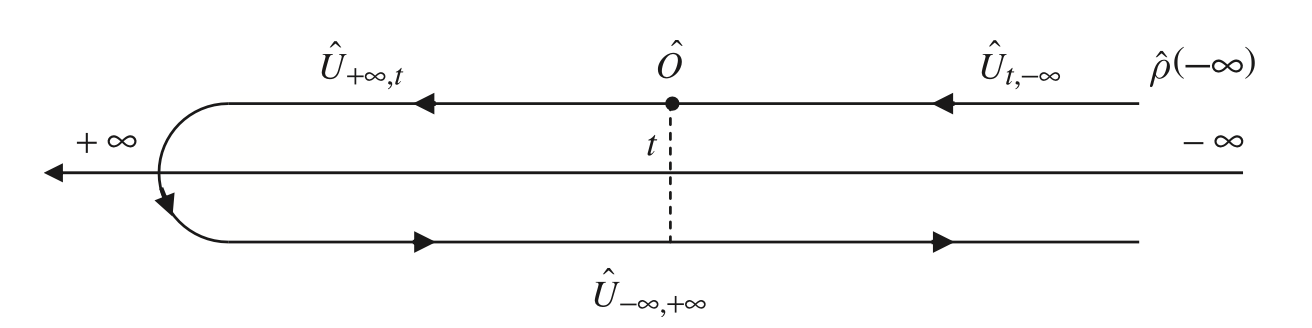
\includegraphics[scale=0.8]{Figures/Time contour.png}
  \caption{时序围道}
\end{figure}
如果密度矩阵是一个热力学系综,那么密度矩阵可写为$ e^{-\beta \hat{H}^{\mathrm{M}}}=e^{-\mathrm{i} \int_{\gamma \mathrm{M}} d \bar{z} \hat{H}^{\mathrm{M}}} $,$ \gamma \mathrm{M} $是复平面上连接任意两点的path,只需满足$ z_b-z_a=-\mathrm{i} \beta $,而$ \hat{H}^{\mathrm{M}}=\hat{H}-\mu \hat{N} $,利用Trace的性质,可以用一个包括$ \gamma_M  $的围道改写
\begin{equation}
  \operatorname{Tr}\left[e^{-\mathrm{i} \int_{t_{0+}}^{z_b} d \bar{z} \hat{H}^{\mathrm{M}}} \mathcal{T}\left\{e^{-\mathrm{i} \int_\gamma d \bar{z} \hat{H}(\bar{z})} \hat{O}(z)\right\} e^{-\mathrm{i} \int_{z_a}^{t_0-} d \hat{z}^{\mathrm{M}}}\right]=\operatorname{Tr}\left[\mathcal{T}\left\{e^{-\mathrm{i} \int_\gamma \mathrm{M} \oplus \gamma} d \bar{z} \hat{H}(\bar{z}) \hat{O}(z)\right\}\right]
\end{equation}    
此时的算符期望值为
\begin{equation*}
  O(z)=\frac{\operatorname{Tr}\left[\mathcal{T}\left\{e^{-\mathrm{i} \int_\gamma d \bar{z} \hat{H}(\bar{z})} \hat{O}(z)\right\}\right]}{\operatorname{Tr}\left[\mathcal{T}\left\{e^{-\mathrm{i} \int_\gamma d \bar{z} \hat{H}(\bar{z})}\right\}\right]}
\end{equation*}
注意到围道不同部分具有不同的哈密顿量
\section{玻色化与JW变换}
\section{自旋-电荷分离}
作为Fractionalization最典型的两个例子之一(另一个是FQHE中的分数电荷),也是准粒子的典型例子之一
\section{H-S变换}
Hubbard–Stratonovich变换是用白噪声涨落的虚拟玻色场解耦合具有相互作用的物质场,此时通过引入一个虚拟玻色场的代价是的物质场的作用量是高斯型的,形式上可以直接做高斯积分,得到仅包含玻色场的有效作用量,在这个有效作用量的基础上更方便对低能激发做分析。考虑相互作用的电子作用量:
\begin{equation}
  S[\psi, \bar{\psi}]=\sum_p \bar{\psi}_{p \sigma}\left(-i \omega_n+\frac{\mathbf{p}^2}{2 m}-\mu\right) \psi_{p \sigma}+\frac{T}{2 L^3} \sum_{p p^{\prime} q} \bar{\psi}_{p+q \sigma} \bar{\psi}_{p^{\prime}-q \sigma^{\prime}} V(\mathbf{q}) \psi_{p^{\prime} \sigma^{\prime}} \psi_{p \sigma}
\end{equation}
现在考虑插入这个一个单位1,
\begin{equation}
  1 \equiv \int D \phi \exp \left[-\frac{e^2 \beta}{2 L^d} \sum_q \phi_q V^{-1}(\mathbf{q}) \phi_{-q}\right]
\end{equation}
积分给出的常数被吸收到了测度的定义中。对积分变量做平移:$ \phi_q \rightarrow \phi_q+i e^{-1} V(\mathbf{q}) \rho_q / \beta $,其中$  \rho_q \equiv \sum_p \bar{\psi}_{p \sigma} \psi_{p+q \sigma}$,得到这样一个看起来麻烦但仍未单位1的量:
\begin{equation}
  1=\int D \phi \exp \left[\frac{1}{L^d} \sum_q\left(-\frac{e^2 \beta}{2} \phi_q V^{-1}(\mathbf{q}) \phi_{-q}+i e \rho_q \phi_{-q}+\frac{1}{2 \beta} \rho_q V(\mathbf{q}) \rho_{-q}\right)\right]
\end{equation}  
可以看到指数中的最后一项刚好和费米子相互作用项抵消,将它乘在原本的配分函数上,得到$ \mathcal{Z}=\int D \phi \int D\left(\bar{\psi}_\sigma, \psi_\sigma\right) e^{-S\left[\phi, \bar{\psi}_\sigma, \psi_\sigma\right]} $,其中作用量为:
\begin{equation}
  S\left[\phi, \bar{\psi}_\sigma, \psi_\sigma\right]=\frac{\beta}{8 \pi L^d} \sum_q \phi_q \mathbf{q}^2 \phi_{-q}+\sum_{p p^{\prime}} \bar{\psi}_{p \sigma}\left[\left(-i \omega_n+\frac{\mathbf{p}^2}{2 m}-\mu\right) \delta_{p p^{\prime}}+\frac{i e}{L^d} \phi_{p^{\prime}-p}\right] \psi_{p^{\prime} \sigma}
\end{equation} 
有时在实空间中的作用量是有用的,有:
\begin{equation}
  S[\phi, \bar{\psi}, \psi]=\int d \tau \int d^d r\left\{\frac{1}{8 \pi}(\partial \phi)^2+\bar{\psi}_\sigma\left[\partial_\tau-\frac{\partial^2}{2 m}-\mu+\frac{i e}{L^d} \phi\right] \psi_\sigma\right\}
\end{equation}
上述形式的物理解释是将电子看作处于外场$ \phi $中,第一项给出电场的能量密度。在上面的例子基础上,对H-S变换做点一般的解释。考虑这样一个双线性相互作用项$ V_{\alpha \beta \gamma \delta} \bar{\psi}_\alpha \psi_\beta \bar{\psi}_\gamma \psi_\delta $,可以引入记号$ \hat{\rho}_{\alpha \beta} \equiv \psi_\alpha \psi_\beta $,再引入$ m \equiv(\alpha \beta), n \equiv(\gamma \delta) $, 将相互作用项改写为$ S_{\mathrm{int}}=\hat{\rho}_m V_{m n} \hat{\rho}_n $。对这项作用量乘上单位1:
\begin{equation}
  e^{-\hat{\rho}_m V_{m n} \hat{\rho}_n}=\underbrace{\int D \phi e^{-\frac{1}{4} \phi_m V_{m n}^{-1} \phi_n}}_1 e^{-\hat{\rho}_m V_{m n} \hat{\rho}_n}
\end{equation}   
做一个变量平移:$ \phi_m \rightarrow \phi_m+2 i(V \hat{\rho})_m $,消掉双线性相互作用项:
\begin{equation}
  \exp \left[-\hat{\rho}_m V_{m n} \hat{\rho}_n\right]=\int D \phi \exp \left[-\frac{1}{4} \phi_m V_{m n}^{-1} \phi_n-i \phi_m \hat{\rho}_m\right]
\end{equation} 
上面的算符选择有一定的任意性:$ \hat{\rho}_{\alpha \beta} $,从四个算符中选取两个出来总共有三种情况,对应于direct channel,exchange channel和Copper channel:
\begin{figure}[htbp]
  \centering
  \includegraphics*[scale=0.7]{channels.png}
  \caption{三种通道,直接、Copper、间接}
\end{figure} 
具体选择哪个通道依赖于物理过程,核心思想是使得积分空间大。将高斯型的费米场积掉,有:
\begin{equation}
  \mathcal{Z}=\int D \phi e^{-\frac{\beta}{8 \pi L^3} \sum_q \phi_q \mathbf{q}^2 \phi_{-q}} \operatorname{det}\left[-i \hat{\omega}+\frac{\hat{\mathbf{p}}^2}{2 m}-\mu+\frac{i e}{L^d} \hat{\phi}\right]
\end{equation}
利用对非奇异算符求迹与对数的一个恒等式:$ \ln \operatorname{det} \hat{A}=\operatorname{tr} \ln \hat{A} $,作用量可以改写为:
\begin{equation}
  S[\phi]=\frac{\beta}{8 \pi L^d} \sum_q \phi_q \mathbf{q}^2 \phi_{-q}-\operatorname{tr} \ln \left[-i \hat{\omega}+\frac{\hat{\mathbf{p}}^2}{2 m}-\mu+\frac{i e}{L^d} \hat{\phi}\right]
\end{equation}
\section{电子体系费曼图的部分求和近似}
费曼图本身按照圈图展开给出了其自然的层级,但通常来说对某一阶圈图的求和依然过于复杂,可以根据实际问题的物理条件选取另外的参数标记图的贡献,并选取作出主要贡献的图,再求和,这相当于选取了全体费曼图中的一无穷子序列。我们在Jellium模型下做探讨,因此$ V(q=o) $的项都没有贡献,也就是说不用考虑一根电子线闭合的情况。 
\subsection{环形图近似or随机相位近似or大N近似}
考察零温的正规自能中不为零的一阶图与二阶图:
\begin{figure}[htbp]
  \centering
  \includegraphics*[scale=0.7]{Figures/正规自能的修正.png}
  \caption{正规自能的修正}
\end{figure}
第一项很容易对频率积分后写出:
\begin{equation}
  \Sigma^{*(1)}(\boldsymbol{k})=-\int \frac{\mathrm{d} \boldsymbol{k}^{\prime}}{(2 \pi)^3} V\left(\boldsymbol{k}-\boldsymbol{k}^{\prime}\right) \theta\left(k_{\mathrm{F}}-k^{\prime}\right)
\end{equation}
代入相互作用的形式,可以计算出:
\begin{equation}
  \begin{aligned}
    \Sigma^{*(1)}(\boldsymbol{k}) & =-\frac{e^2}{\varepsilon_0(2 \pi)^3} \int \mathrm{d} \boldsymbol{k}^{\prime} \frac{\theta\left(k_{\mathrm{F}}-k^{\prime}\right)}{\left|\boldsymbol{k}-\boldsymbol{k}^{\prime}\right|^2} \\
    & =-\frac{e^2}{\varepsilon_0(2 \pi)^3 \varepsilon_0 k} \int_0^{k_{\mathrm{F}}} k^{\prime 2} \mathrm{~d} k^{\prime} \int_0^{2 \pi} \mathrm{d} \varphi \int_0^\pi \frac{\mathrm{d} \theta}{k^2+k^{\prime 2}-2 k k^{\prime} \cos \theta} \\
    & =-\frac{e^2}{(2 \pi)^3 \varepsilon_0 k} \int_0^{k_{\mathrm{F}}} k^{\prime} \mathrm{d} k^{\prime} \ln \left|\frac{k+k^{\prime}}{k-k^{\prime}}\right|=-\frac{e^2}{4 \pi^2 \varepsilon_0} k_{\mathrm{F}}\left(1+\frac{k_F^2-k^2}{2 k k_{\mathrm{F}}} \ln \left|\frac{k_{\mathrm{F}}+k}{k_{\mathrm{F}}-k}\right|\right)
    \end{aligned}
\end{equation}
可以通过幂次分析得到这项是收敛还是发散:零温格林函数的频率积分给出$ \theta\left(k_{\mathrm{F}}-k^{\prime}\right) $,这相当于限制了q的积分区域,相互作用项给出$ \sim\frac{1}{q^2} $,积分为$ dq^3 $,因此是收敛的。但之后的一些图在$ q\to 0 $的情况下发散,用费曼规则写出它们对应的积分并做幂次分析得出:
\begin{equation}
  \begin{aligned}
    & \frac{1}{\mathrm{i} \hbar} \Sigma_{\mathrm{r}}^{*(2)}(\boldsymbol{k}, \omega)=-\frac{1}{(2 \pi)^8} \int \mathrm{d}^4 p \mathrm{~d}^4 q \mathrm{i} G^0(k-q) \mathrm{i} G^0(p+q) \mathrm{i} G^0(p) \\
    & \times\left(\frac{1}{\mathrm{i} \hbar}\right)^2 V^2(\boldsymbol{q}) \propto \int \frac{\mathrm{d}^3 q}{q^4} \sim \frac{1}{q} \rightarrow \infty \\
    & \frac{1}{\mathrm{i} \hbar} \Sigma_{\mathrm{b}}^{*(2)}(\boldsymbol{k}, \omega)=\frac{1}{(2 \pi)^8} \frac{\mathrm{i}^3}{(\mathrm{i} \hbar)^2} \int \mathrm{d}^4 p \mathrm{~d}^4 q G^0(k-p)(k-q) G^0(k-p-q) \\
    & \times V(\boldsymbol{p}) V(\boldsymbol{q}) \propto \int \frac{\mathrm{d}^3 p}{p^2} \int \frac{\mathrm{d}^3 q}{q^2} \\
    & \frac{1}{\mathrm{i} \hbar} \Sigma_{\mathrm{c}}^{*(2)}(\boldsymbol{k}, \omega)=\frac{1}{(2 \pi)^8} \frac{\mathrm{i}^3}{(\mathrm{i} \hbar)^2} \int \mathrm{d}^4 p \mathrm{~d}^4 q \mathrm{i} V(\boldsymbol{q}) V(\boldsymbol{p}) \\
    & \times\left[G^0(k-q)\right]^2 G^0(k-p-q) \mathrm{e}^{\mathrm{i}\left(k_0-p_0-q_0\right) 0^{+}} \propto \int \frac{\mathrm{d}^3 p}{p^2} \int \frac{\mathrm{d}^3 q}{q^2} \\
    &
    \end{aligned}
\end{equation}   
可以看到后两项收敛,因此主要贡献为第一项,即对相互作用线修正的项红外发散,观察其发散特征来自两根相互作用线传播的动量是相同的,而传播子总是在费米动量处有最大的贡献,这相当于对每条传播子给出一限制,环形图的相互作用线的动量总是一样的,使得它积分动量的空间比其他图更大,给出更大的贡献。这也可以从表达式看出,对于N个相互作用线传播的动量是相同的的情况,积分中出现$ \int d^3q\frac{1}{(q^2)^N} $,而传播动量不同的图给出$ \int d^3q_1\frac{1}{q_1^2}\int d^3q_2\frac{1}{q_2^2}\dots $,在$ q\to0 $时的发散总是要更小。\\

环形图近似就是说在每级圈图中,只考虑求和发散程度最大的环形图\footnote{高阶圈图的非环形图发散程度会比低阶圈图的环形图更高,为何不考虑?因为它总是被假设为很小的相互作用系数给压低了,虽然对高阶无穷大乘以有限小的量看起来并不合理,但该论述的核心是只能在同阶圈图中比较发散大小。},而这样的图的单粒子不可约图是很简单的,再利用Schwinger–Dyson方程就给出总贡献。在环形图近似中,只考虑了相互作用线的修正,并且修正的单粒子不可约图只考虑单环形图,我们需要给出这个近似的适用条件,即满足$ \Pi^{*(0)} \gg \Pi^{*(n)}, n=1,2, \cdots, \infty $的条件。
\begin{figure}[htbp]
  \centering
  \includegraphics*[scale=0.7]{Figures/极化的一阶图和二阶图.png}
  \caption{极化的一阶图和二阶图}
\end{figure} 
一阶图和二阶图的式子为:
\begin{equation}
  \mathrm{i} \hbar \Pi^0(q)=\mathrm{i} \hbar \Pi^{*(0)}(q)=-2 \mathrm{i}^2 \int \frac{\mathrm{d}^4 p}{(2 \pi)^4} G^0(p+q) G^0(p)
\end{equation}
\begin{equation}
  \mathrm{i} \hbar \Pi^{*(1)}(q)=-2 \frac{\mathrm{i}^4}{\mathrm{i} \hbar} \frac{1}{(2 \pi)^8} \int \mathrm{d}^4 p_1 \mathrm{~d}^4 p_2 G^0\left(p_1\right) G^0\left(p_1+q\right) G^0\left(p_2\right) G^0\left(p_2+q\right) V\left(\boldsymbol{p}_2-\boldsymbol{p}_1\right)
\end{equation}
先估计$ \hbar \Pi^{*(1)}(q) $的大小,它是红外发散的,只有在$ q\to0 $的值是主要的,此时$ V\left(\boldsymbol{p}_2-\boldsymbol{p}_1\right) $可以近似为$ e^2 / \varepsilon_0 k_{\mathrm{F}}^2 $,这是因为当q很小时,要求上面的格林函数取费米动量时,$ \boldsymbol{p}_2-\boldsymbol{p}_1\sim0\to2k_F $,于是积分估计为:
\begin{equation}
  \begin{aligned}
    \mathrm{i} \hbar \Pi^{*(1)}(q) & \sim-2 \frac{\mathrm{i}^4}{\mathrm{i} \hbar} \frac{1}{(2 \pi)^8} \frac{e^2}{\varepsilon_0 k_{\mathrm{F}}^2} \int \mathrm{d}^4 p_1 \mathrm{~d}^4 p_2 G^0\left(p_1\right) G^0\left(p_1+q\right) G^0\left(p_2\right) G^0\left(p_2+q\right) \\
    & =-\frac{2}{\mathrm{i} \hbar} \frac{e^2}{\varepsilon_0 k_{\mathrm{F}}^2}\left[\mathrm{i} \hbar \Pi^{*(0)}\right]^2=-2 \mathrm{i} \hbar \frac{e^2}{\varepsilon_0 k_{\mathrm{F}}^2}\left(\Pi^{*(0)}\right)^2
    \end{aligned}
\end{equation}   
接下来详细计算$ \Pi^0(q) $,它其实用有限温度的技术更好算,也就是计算极化算符$ \Pi_q \equiv \frac{2 T}{L^3} \sum_p G_p G_{p+q} $,利用松原求和解决频率部分得到:
\begin{equation}
  \Pi_q=\frac{2 T}{L^3} \sum_p \frac{1}{-i \omega_n+\xi_{\mathbf{p}}} \frac{1}{-i \omega_{n+m}+\xi_{\mathbf{p}+\mathbf{q}}}=\frac{2}{L^3} \sum_{\mathbf{p}} \frac{n_{\mathrm{F}}\left(\epsilon_{\mathbf{p}+\mathbf{q}}\right)-n_{\mathrm{F}}\left(\epsilon_{\mathbf{p}}\right)}{i \omega_m+\xi_{\mathbf{p}+\mathbf{q}}-\xi_{\mathbf{p}}}
\end{equation}
接下来就是对动量求和,由于式子中的费米分布函数,积分的主要贡献在费米动量附近,可以取$ |\mathbf{p}| \simeq p_{\mathrm{F}},|\mathbf{q}| \ll p_{\mathrm{F}} $,此时可对能量差做线性近似$ \xi_{\mathbf{p}+\mathbf{q}}-\xi_{\mathbf{p}}=(1 / m) \mathbf{p} \cdot \mathbf{q}+\mathcal{O}\left(q^2\right) $,同样地对于分布函数有$ n_{\mathrm{F}}\left(\epsilon_{\mathbf{p}+\mathbf{q}}\right)-n_{\mathrm{F}}\left(\epsilon_{\mathbf{p}}\right) \simeq \partial_{\epsilon_p} n_{\mathrm{F}}\left(\epsilon_p\right)(1 / m) \mathbf{p} \cdot \mathbf{q} \simeq-\delta\left(\epsilon_p-\mu\right)(1 / m) \mathbf{p} \cdot \mathbf{q} $,最终取零温极限将求和转化为积分最终对于三维各向同性的情况,它给出Lindhard函数:
\begin{equation}
  \begin{aligned}
    \Pi_{\mathbf{q}, \omega_m} & =-\frac{2}{(2 \pi)^3} \int d p p^2 \int d \Omega \delta\left(\epsilon_p-\mu\right) \frac{v_{\mathrm{F}} \mathbf{n} \cdot \mathbf{q}}{i \omega_m+v_{\mathrm{F}} \mathbf{n} \cdot \mathbf{q}} \\
    & =-\underbrace{\frac{2}{(2 \pi)^3} \int d p p^2 \int d \Omega \delta\left(\epsilon_p-\mu\right)}_{\nu_0} \frac{1}{\int d \Omega} \int d \Omega \frac{v_{\mathrm{F}} \mathbf{n} \cdot \mathbf{q}}{i \omega_m+v_{\mathrm{F}} \mathbf{n} \cdot \mathbf{q}} \\
    & =-\frac{\nu_0}{2} \int_{-1}^1 d x \frac{v_{\mathrm{F}} x q}{i \omega_m+v_{\mathrm{F}} x q}=-\nu_0\left[1-\frac{i \omega_m}{2 v_{\mathrm{F}} q} \ln \left(\frac{i \omega_m+v_{\mathrm{F}} q}{i \omega_m-v_{\mathrm{F}} q}\right)\right] .
    \end{aligned}
\end{equation}  
当$ q\to0 $时,$ \mathrm{i} \hbar \Pi^0 \sim m k_{\mathrm{F}} /\left(\pi \hbar^2\right) $,因此环形图近似的条件为:
\begin{equation}
  \frac{\Pi^{*(1)}(q)}{\Pi^0(q)} \sim \frac{e^2}{\varepsilon_0 k_{\mathrm{F}}^2} \Pi^{*(0)} \sim \frac{m e^2}{4 \pi \varepsilon_0 \hbar^2 k_{\mathrm{F}}}=\frac{1}{k_{\mathrm{F}} a_0} \ll 1
\end{equation}
也就是高密度条件。利用Schwinger-Dyson方程给出有效作用:
\begin{equation}
  U_{\mathbf{r}}(q)=\frac{V(\boldsymbol{q})}{1-V(\boldsymbol{q}) \Pi^0(q)}=\frac{e^2 / \varepsilon_0}{|\boldsymbol{q}|^2-e^2 \Pi^0(q) / \varepsilon_0}
\end{equation}  
从物理上来说,对费曼图的部分求和将库伦作用修正为短程作用,并且有效作用含频率,因此是推迟势。\\

环形图近似也可以从大N展开+只考虑相互作用线修正得到。将自旋指标S作为一个参量,并将相互作用系数除以(2S+1)\footnote{这并不改变物理,只是和前面的注释一样,这便于我们分析不同阶圈图中的不同阶(2S+1)图},而费曼规则告诉我们,每有一个物质粒子圈就给出指标求和$ (2S+1) $,因此相互作用线修正中不同图的系数如图所示
\begin{figure}[htbp]
  \centering
  \includegraphics*[scale=0.5]{Figures/大N展开.png}
  \caption{相互作用线修正中不同图的系数}
\end{figure}
\\ 
前面所说的环形图近似只考虑量级为N的第一张图。\\

当考虑粒子线的修正时,大N展开就给出了Non-Crossing Approximation,这是一种部分求和粒子线自能图的近似。
\begin{figure}[htbp]
  \centering
  \includegraphics*[scale=0.5]{Figures/电子自能的NCA.png}
  \caption{电子自能的NCA}
\end{figure}
图中单粒子闭合线由于选取了$ V(q=0)=0 $而不考虑,图中给出了交叉图与非交叉图对指标的求和,可以看出在同阶圈图中非交叉图总是给出最多次的指标求和,因此占据主导。但此时的单粒子不可约图仍旧为无限个,不能简单的像RPA直接求解,而是需要求和所有“彩虹图”,最后得到自洽方程。 
\section{费米液体}
\subsection{传统推导}
\subsubsection{准粒子}
准粒子的概念是朗道费米液体理论的核心,它将无相互作用时的自由粒子激发与有相互作用时费米面附近的激发通过绝热演化一一对应起来。无
相互作用的费米气的态矢可以用占据数标记:
\begin{equation}
	\Psi=\left|n_{\mathrm{p}_1 \sigma_1}, n_{\mathrm{p}_2 \sigma_2}, \ldots\right\rangle
\end{equation}
它的基态就是我们熟知的费米能以下都被占据:
\begin{equation}
	\text { ground state } \Psi_0 \quad: \quad n_{\mathrm{p} \sigma}= \begin{cases}1 & \left(p<p_F\right) \\ 0 & \text { (otherwise). }\end{cases}
\end{equation}
在不发生相变的假设下,此基态在绝热演化打开相互作用时会变为相互作用体系的基态,相互作用的基态能量未知,记为$ E_0 $。\\
当在费米面上添加一电子并继续上述的绝热演化操作时,由于相互作用,这并非一个能量本征态,会由于发射电子-空穴对而衰变到其他态,但只要
这个电子的寿命$ \tau(\epsilon) \sim \epsilon^{-2} $远大于绝热演化的时间$ \tau_A=\epsilon^{-1} $我们就会引入一个量级为$ \tau^{-1}\left(\epsilon_{\mathbf{p}}\right) /\left|\epsilon_{\mathbf{p}}\right| \propto\left|\epsilon_{\mathbf{p}}\right| $
的误差,当只考虑费米面附近微扰时这误差可以忽略。绝热演化是动量守恒的,记末态为:
\begin{equation}
	\text { quasiparticle : } \Psi_{\mathbf{p}_0 \sigma_0} \quad n_{\mathrm{p} \sigma}= \begin{cases}1 & \left(p<p_F \text { or } \mathbf{p}=\mathbf{p}_0, \sigma=\sigma_0\right) \\ 0 & \text { (otherwise) }\end{cases}
\end{equation}    
可以看出绝热演化保持费米动量不变。这是一个准粒子单态,称为准粒子是在之后可以看到它表现的几乎就像一个粒子。此准粒子耗费能量为:$ E_{\mathbf{p}_0}^{(0)}=E\left(p_0\right)-E_0 $,
在巨正则系综下减去化学势的能量更加好用:$ \epsilon_{\mathbf{p}_0}^{(0)}=E_{\mathbf{p}_0}^{(0)}-\mu=\mathcal{E}\left(p_0\right)-\mathcal{E}_0 $。对于空穴同理。\\
当准粒子处于费米面上时,可散射的相空间为零,因此费米面上的占据数是一个守恒量:
\begin{equation}
	\left[H, n_{\mathbf{p}_F \sigma}\right]=0 . \quad\left(\mathbf{p}_F \in \mathrm{FS}\right)
\end{equation}  
现在问题就是用上述的一系列守恒量去描述自由能以及动力学。对于稀疏的费米液体,能量可以用占据数相较基态的偏移量展开:
\begin{equation}
	\mathcal{E}=\mathcal{E}_0+\sum_{\mathbf{p} \sigma}\left(E_{\mathbf{p} \sigma}^{(0)}-\mu\right) \delta n_{\mathbf{p} \sigma}+\frac{1}{2} \sum_{\mathbf{p}, \mathbf{p}^{\prime}, \sigma, \sigma^{\prime}} f_{\mathbf{p} \sigma, \mathbf{p}^{\prime} \sigma^{\prime}} \delta n_{\mathbf{p} \sigma} \delta n_{\mathbf{p}^{\prime} \sigma^{\prime}}+\cdots .
\end{equation}
在费米面附近,准粒子的能量可以作线性近似:$ E_p^{(0)}=v_F\left(p-p_F\right)+\mu^{(0)} $,可以利用费米速度定义有效质量:
\begin{equation}
	v_F=\left.\frac{d \epsilon_p^{(0)}}{d p}\right|_{p=p_F}=\frac{p_F}{m^*}
\end{equation}
二阶系数$ f_{\mathbf{p} \sigma, \mathbf{p}^{\prime} \sigma^{\prime}}=\left.\frac{\delta^2 \mathcal{E}}{\delta n_{\mathbf{p} \sigma} \delta n_{\mathbf{p}^{\prime} \sigma^{\prime}}}\right|_{\delta n_{\mathbf{p}^{\prime \prime} \sigma^{\prime \prime}}=0} $描述了
费米面上的准粒子之间的相互作用。由于绝热演化不改变占据数,熵也不改变:
\begin{equation}
	S=-k_B \sum_{\mathbf{p}, \sigma}\left[n_{\mathbf{p} \sigma} \ln n_{\mathbf{p} \sigma}+\left(1-n_{\mathbf{p} \sigma}\right) \ln \left(1-n_{\mathbf{p} \sigma}\right)\right]
\end{equation}
于是自由能为:
\begin{equation}
	\begin{aligned}
		F\left(\left\{n_{\mathbf{p} \sigma}\right\}\right)= & \mathcal{E}_0(\mu)+\sum_{\mathbf{p} \sigma} \epsilon_{\mathbf{p} \sigma}^{(0)} \delta n_{\mathbf{p} \sigma}+\frac{1}{2} \sum_{\mathbf{p}, \mathbf{p}^{\prime}, \sigma, \sigma^{\prime}} f_{\mathbf{p} \sigma, \mathbf{p}^{\prime} \sigma^{\prime}} \delta n_{\mathbf{p} \sigma} \delta n_{\mathbf{p}^{\prime} \sigma^{\prime}} \\
		& +k_B T \sum_{\mathbf{p}, \sigma}\left[n_{\mathbf{p} \sigma} \ln n_{\mathbf{p} \sigma}+\left(1-n_{\mathbf{p} \sigma}\right) \ln \left(1-n_{\mathbf{p} \sigma}\right)\right] .
		\end{aligned}
		\label{HFE}
\end{equation}
\subsubsection{中性费米液体}
考虑各向同性、短程相互作用的中性费米液体
当相互作用在自旋空间中的转动不变时,$ f_{\mathbf{p} \sigma} $的形式可以化简。上面所写出的占据数$ n_{\mathbf{p} \sigma }$实际上是
自旋空间中的密度矩阵$ n_{\mathbf{p} \alpha\beta} $的对角元,可观测量的期望由它与对应算符的迹给出,如自旋期望值:$  \sigma_p=\frac{1}{2} \sum_{\alpha \bar{a}}(\tau)_{\alpha \bar{\alpha}}\left(n_p\right)_{\bar{\alpha} \alpha}$,
此时二阶系数自旋不变时可以写为:$ f_{\mathbf{p} \alpha \beta ; \mathbf{p}^{\prime} \gamma \eta}=f^s\left(\mathbf{p}, \mathbf{p}^{\prime}\right) \delta_{\alpha \beta} \delta_{\gamma \eta}+f^a\left(\mathbf{p}, \mathbf{p}^{\prime}\right) \vec{\sigma}_{\alpha \beta} \cdot \vec{\sigma}_{\gamma \eta} $,
取其对角元$ \alpha=\beta=\sigma,\gamma=\eta=\sigma^\prime $,有系数的形式:
\begin{equation}
	f_{\mathbf{p} \sigma, \mathbf{p}^{\prime} \sigma^{\prime}}=f_{\mathbf{p}, \mathbf{p}^{\prime}}^s+f_{\mathbf{p}, \mathbf{p}^{\prime}}^a \sigma \sigma^{\prime}
\end{equation}   
实际上只关心费米面附近的激发,因此取$ \mathbf{p}=p_F \hat{\mathbf{p}},\mathbf{p^\prime}=p_F \hat{\mathbf{p^\prime}} $,在各向同性的相互作用中,系数只与两个动量的夹角有关
$ f_{\mathbf{p}, \mathbf{p}^{\prime}}^{s, a}=f^{s, a}(\cos \theta) $,乘上态密度将变成一个无量纲数,这是更加方便的,因此定义:
\begin{equation}
	F^{s, a}(\cos \theta)=\mathcal{N}^*(0) f^{s, a}(\cos \theta)
\end{equation}  
总可以将上述系数用Legendre多项式展开,
\begin{equation}
	F^{s, a}(\cos \theta)=\sum_{l=0}^{\infty}(2 l+1) F_l^{s, a} P_l(\cos \theta)
\end{equation}
展开系数就称为Landau因子。对于前面求出的自由能\eqref{HFe},当占据数的变化很小时,由热力学平衡条件有:
\begin{equation}
	\delta F=\sum_{\mathbf{p} \sigma} \delta n_{\mathbf{p} \sigma}\left[\epsilon_{\mathbf{p} \sigma}+k_B T \ln \left(\frac{n_{\mathbf{p} \sigma}}{1-n_{\mathbf{p} \sigma}}\right)\right]+O\left(\delta n_{\mathbf{p} \sigma}^2\right)=0
\end{equation} 
于是有$ n_{\mathbf{p} \sigma}=\frac{1}{e^{\beta \epsilon_{\mathbf{p} \sigma}}+1}=f\left(\epsilon_{\mathbf{p} \sigma}\right) $,但由于$ \epsilon_{\mathbf{p} \sigma} $是占据数的函数,因此上式给出个占据数的隐函数解,但对于
$ T\to 0 $时它就和普通的F-D分布一样了。\\

当考虑对系统外加场时,此时能量的变化有两部分,一是单粒子能量的改变,二是占据数的改变:
\begin{equation}
	\delta \epsilon_{\mathbf{p} \sigma}=\delta \epsilon_{\mathbf{p} \sigma}^{(0)}+\sum_{\mathbf{p}^{\prime} \sigma^{\prime}} f_{\mathbf{p} \sigma \mathbf{p}^{\prime} \sigma^{\prime}} \delta n_{\mathbf{p}^{\prime} \sigma^{\prime}}
\end{equation}
同时占据数的改变本身依赖于能量的改变,这给出一个自洽方程,同时考虑低温近似,F-D分布函数可以视为theta函数\footnote{注意分辨delta函数与占据数的偏移量}:
\begin{equation}
	\delta \epsilon_{\mathbf{p} \sigma}=\delta \epsilon_{\mathbf{p} \sigma}^{(0)}-\sum_{\mathbf{p}^{\prime} \sigma^{\prime}} f_{\mathbf{p} \sigma \mathbf{p}^{\prime} \sigma^{\prime}} \delta\left(\epsilon_{\mathbf{p}^{\prime}}^{(0)}\right) \delta \epsilon_{\mathbf{p}^{\prime} \sigma}
\end{equation}
为求解这个自洽性方程,自然地拟设解具有同样的对称性:$ \delta \epsilon_{\mathbf{p} \sigma}=t_l Y_{l m}(\hat{\mathbf{p}}) $,最终有:
\begin{equation}
	t_l=\frac{v_l}{1+F_l^s}
\end{equation} 
\subsection{质量重整化}
假设粒子携带某种守恒荷并与外矢量场耦合,微观的哈密顿量为:
\begin{equation}
	H\left[\mathbf{A}_N\right]=\sum_\sigma \int d^3 x \frac{1}{2 m} \psi_\sigma^{\dagger}(x)\left[\left(-i \hbar \nabla-\mathbf{A}_N\right)^2\right] \psi_\sigma(x)+\hat{V}
\end{equation}
在一阶近似下,能量的改变量为:$ \delta \hat{H}=-\mathbf{A}_N \cdot \frac{\hat{\mathbf{P}}}{m} $,对于无相互作用并且给定占据数的体系有:
\begin{equation}
	\delta E=\langle\delta H\rangle=-\frac{\langle\mathbf{P}\rangle}{m} \cdot \mathbf{A}_N=-\sum_{\mathbf{p} \sigma}\left(\frac{\mathbf{p}}{m} \cdot \mathbf{A}_N\right) n_{\mathbf{p} \sigma}
\end{equation} 
单粒子能量的改变为:$ \delta \epsilon_{\mathbf{p} \sigma}^{(0)}=-\frac{\mathbf{p}}{m} \cdot \mathbf{A}_N=-A_N \frac{p_F}{m} \cos \theta $,这是一个偶极矩作用。对于朗道费米液体,总的能量改变量为:
\begin{equation}
	\delta \epsilon_{\mathbf{p} \sigma}=-\frac{\mathbf{p}}{m^*} \cdot \mathbf{A}_N=-A_N \frac{p_F}{m^*} \cos \theta
\end{equation} 
不难得出$ \frac{m}{m^*}=\frac{1}{1+F_1^s} $。 
\subsubsection{朗道费米液体的微观基础}
朗道费米液体理论是一个唯象理论,它的正确性可从微观角度说明。
\subsection{从有效场论的角度}
固体中的电子的性质依赖于一下参数$ e,\hbar,m $,可以构造一个特征能量:$ e^4 m / \hbar^2=27 \mathrm{eV} $,事实上导带中的电子能量会略小$ E_0\sim(1,10)eV $。实际上理论中还会出现参数$ M,c $,它们相较于其他参数
都太大了,可以视作无穷。\\
对于导体,任意微小的电场都会激发出电流,因此荷激发是没有能隙的,这使得我们能够研究$ E<<E_0 $的有效理论。按照有效场论的精神,写下满足对称性的最一般的拉格朗日量,再对它的形式作出猜测,最终与实验比较验证。在此猜测带电的轻场和真正的电子都是自旋$ \frac{1}{2} $的费米子,自由作用量为:
\begin{equation}
	\int d t d^3 \mathbf{p}\left\{i \psi_\sigma^{\dagger}(\mathbf{p}) \partial_t \psi_\sigma(\mathbf{p})-\left(\varepsilon(\mathbf{p})-\varepsilon_{\mathrm{F}}\right) \psi_\sigma^{\dagger}(\mathbf{p}) \psi_\sigma(\mathbf{p})\right\}
\end{equation}     
其中不对$ \varepsilon(\mathbf{p}) $形式作出要求以体现一般性。现在我们考虑,当能标重标度s时,场怎么变化。和相对论情形中动量和能量一起重标度不同,在此当能量重标度趋于零时,动量重标度趋于费米动量。因此将动量重写为:$ \mathbf{p}=\mathbf{k}+\mathbf{l} $,$ \mathbf{k} $是费米面上的动量,$ \mathbf{l} $垂直于费米面,因此,当$ E\to sE $时,$ \mathbf{k}\to\mathbf{k},\mathbf{l}\to s\mathbf{l} $。对于单粒子能量,在费米面附近做线性展开:
\begin{equation}
	\varepsilon(\mathbf{p})-\varepsilon_{\mathrm{F}}=l v_{\mathrm{F}}(\mathbf{k})+O\left(l^2\right)
\end{equation} 
做标度:
\begin{equation}
	d t \rightarrow s^{-1} d t, \quad d \mathbf{k} \rightarrow d \mathbf{k}, \quad d \mathbf{l} \rightarrow s d \mathbf{l}, \quad \partial_t \rightarrow s \partial_t, \quad l \rightarrow s l
\end{equation}    
通过量纲分析很容易发现场随标度s的变化为$ s^{-\frac{1}{2}} $ 
\section{电、声子有效相互作用}
\section{Goldstone定理(经典)}
考虑一个理论涉及若干个场$ \phi^a(x) $,具有如下形式的拉氏量:
\begin{equation}
  \mathcal{L}=(\text { terms with derivatives })-V(\phi)
\end{equation}
令$ \phi^0_a $为最小化V的恒定场,即
\begin{equation*}
  \left.\frac{\partial}{\partial \phi^a} V\right|_{\phi^a(x)=\phi_0^a}=0 .
\end{equation*} 
将V在极小值附近展开,有:
\begin{equation*}
  V(\phi)=V\left(\phi_0\right)+\frac{1}{2}\left(\phi-\phi_0\right)^a\left(\phi-\phi_0\right)^b\left(\frac{\partial^2}{\partial \phi^a \partial \phi^b} V\right)_{\phi_0}+\cdots .
\end{equation*}
定义取二次项的系数作为矩阵,由于是在极小值展开,矩阵是半正定的,本征值就是质量。下面开始正式证明Goldstone定理。
考虑某一般的连续对称变换:
\begin{equation}
  \phi^a \longrightarrow \phi^a+\alpha \Delta^a(\phi)
\end{equation}
$ \alpha $是无限小参数,$ \Delta^a $是一个关于所有场的函数。考虑退化到恒定场的情况,此时含导数项自动为零,因此势能本身就需要不变,即
\begin{equation*}
  \Delta^a(\phi) \frac{\partial}{\partial \phi^a} V(\phi)=0
\end{equation*} 
此式再对$ \phi^b $求导,并取$ \phi=\phi_0 $:
\begin{equation*}
  0=\left(\frac{\partial \Delta^a}{\partial \phi^b}\right)_{\phi_0}\left(\frac{\partial V}{\partial \phi^a}\right)_{\phi_0}+\Delta^a\left(\phi_0\right)\left(\frac{\partial^2}{\partial \phi^a \partial \phi^b} V\right)_{\phi_0}
\end{equation*}   
由于$ \phi_0 $使得V最小,第一项自动为0,因此第二项也等于零。若对称性依然对于场$ \phi_0 $成立,$ \Delta^a(\phi_0)=0 $。若发生自发对称性破缺,则二阶导项为零,即质量为零。   

\section{Multipartite Entanglement}
\chapter{量子场论}
  \section{同一粒子的不同表示}
\section{Dirac,Weyl and Majorana fermions}\cite{pal2011dirac}
简单来讲,Dirac fermion是Dirac方程的一般解,Majorana fermion是Dirac方程的“实”解,Weyl fermion是无质量Dirac方程的解。\\
\subsection{Dirac方程及其解}
Dirac方程定义为:
\begin{equation}
  \left(i \gamma^\mu \partial_\mu-m\right) \Psi=0\label{de}
\end{equation}
它可以看作具有如下哈密顿量的薛定谔方程:
\begin{equation}
  H=\gamma^0\left(\gamma^i p^i+m\right)
\end{equation}
$\gamma$ 矩阵定义为:
\begin{equation}
  \begin{aligned}
    & {\left[\gamma^\mu, \gamma^\nu\right]_{+}=2 g^{\mu \nu},} \\
    & \gamma_0 \gamma_\mu \gamma_0=\gamma_\mu^{\dagger}
    \end{aligned}
\end{equation}
可以看到,当$ \gamma $矩阵为纯虚时,Dirac方程为实方程,有实解。我们可以找到一组$ \gamma $矩阵 满足这样的条件,这个表象称为Majorana表象。
\begin{equation}
  \begin{array}{ll}
    \widetilde{\gamma}^0=\left[\begin{array}{cc}
    0 & \sigma^2 \\
    \sigma^2 & 0
    \end{array}\right], \quad \widetilde{\gamma}^1=\left[\begin{array}{cc}
    i \sigma^1 & 0 \\
    0 & i \sigma^1
    \end{array}\right], \\
    \tilde{\gamma}^2=\left[\begin{array}{cc}
    0 & \sigma^2 \\
    -\sigma^2 & 0
    \end{array}\right], \quad \tilde{\gamma}^3=\left[\begin{array}{cc}
    i \sigma^3 & 0 \\
    0 & i \sigma^3
    \end{array}\right],
    \end{array}
\end{equation}
其中$ \sigma^i $为Pauli矩阵。在此表象下写出Dirac方程,我们有实解:
\begin{equation}
  \widetilde{\psi}=\tilde{\psi}^{\star}\label{rc}
\end{equation} 
此解即代表Majorana fermion。$ \gamma $矩阵 不同表示之间通过幺正变换相联系:
\begin{equation}
  \gamma^\mu=U \tilde{\gamma}^\mu U^{\dagger}
\end{equation}
此时解$ \tilde{\Psi} $与Majorana表象下的解也通过一个幺正矩阵相联系:
\begin{equation}
  \Psi=U \tilde{\Psi}
\end{equation} 
实解条件\eqref{rc}此时为
\begin{equation}
  \psi=U U^{\top} \psi^{\star}
\end{equation}
我们一般不直接使用幺正矩阵$ U $,而是转而定义如下矩阵:
\begin{equation}
  U U^{\top}=\gamma_0 C
\end{equation} 
由此定义协变共轭(协变性将在稍后证明):
\begin{equation}
  \hat{\Psi} \equiv \gamma_0 C \Psi^{\star}\label{ccg}
\end{equation}
此时实解条件\eqref{rc}可以写为:
\begin{equation}
  \hat{\psi}=\psi\label{grc}
\end{equation}
\subsection{Fourier展开}
一个Majorana fermion解在一般的表象下的Fourier展开为:
\begin{equation}
  \psi(x)=\sum_s \int_p\left(a_s(p) u_s(p) e^{-i p \cdot x}+a_s^{\dagger}(p) v_s(p) e^{+i p \cdot x}\right)
\end{equation}
v和u互为协变共轭$ v_s(p)=\gamma_0 C u_s^{\star}(p) $
\subsection{矩阵C的一些性质}
除了通过找到实解对应的Majorana表象外,我们还可以通过研究 C矩阵本身的性质来定义一组C矩阵,再由此找到不依赖于表象的“实解”条件。\\
简单观察可以发现,C矩阵满足如下性质:
\begin{equation}
  C^{-1} \gamma_\mu C=-\left(U \tilde{\gamma}_\mu U^{\dagger}\right)^{\top}=-\gamma_\mu^{\top}
\end{equation} 
事实上,对于任何表象的$ \gamma $矩阵 我们总可以找到满足上式的C矩阵,此式可以直接称为C矩阵的定义,由此我们有一般情况的实解条件\eqref{grc}
  同时,很容易验证C矩阵在任意表象下都是完全反对称矩阵。
\subsection{实条件的洛伦兹不变性}
此节将阐述为什么称\eqref{ccg}为协变共轭,我们取Lorentz变换的生成元为$ \sigma^{\mu\nu}=\frac{i}{2}[\gamma_\mu,\gamma_\nu]  $,注意,这并非Pauli矩阵。一个fermion场的变换为:
\begin{equation}
  \Psi^{\prime}\left(x^{\prime}\right)=\exp \left(-\frac{i}{4} \omega^{\mu \nu} \sigma_{\mu \nu}\right) \Psi(x)
\end{equation}
对上式取复共轭并左乘$ \gamma_0C $,注意到$ \gamma $矩阵 的性质,可以推出:
\begin{equation}
  \widehat{\Psi}^{\prime}\left(x^{\prime}\right)=\exp \left(-\frac{i}{4} \omega^{\mu \nu} \sigma_{\mu \nu}\right) \widehat{\Psi}(x)
\end{equation} 
由此可以看出,协变共轭场于原场具有相同的洛伦兹变换规则,所以实解条件是洛伦兹不变的。
\subsection{左与右}
在处理费米场时,我们通常会遇到两个和左右有关的概念,螺旋度(helicity)和手性(chirality),两者通常并不相同,但在某些情况下又有关联,本节将阐述这种关联。
\paragraph*{螺旋度}
满足Dirac方程的费米子额度螺旋度定义为:
\begin{equation}
  h_p=\frac{\mathbf{\Sigma} \cdot \mathbf{p}}{\mathrm{p}}
\end{equation}
$ \mathbf{\Sigma} $为自旋矩阵。很显然,$ h_p $的本征值为$ \pm $  1,分别对应“右手”和“左手”。可以验证  $ h_p $与哈密顿量对易,也就是说它是一个守恒量,并且其点乘结构也保证了旋转不变形,但可以验证对于有质量粒子,螺旋度在推动下是改变的。
一个简单的论证是考虑螺旋度的物理意义:自旋在动量方向上的投影,考虑在粒子速度方向上一运动更快的参考系,此时动量反号,但自旋投影在该boost下不改变,因此螺旋度改变。
上面的论述依赖于速度更快的参考系,这对无质量粒子是不可能的,因此这暗示无质量粒子的螺旋度是一个真正的洛伦兹不变量。
\paragraph*{手性}
可以额外定义一个矩阵$ \gamma_5 $,它满足:
\begin{equation}
  \left[\gamma_5, \gamma_\mu\right]_{+}=0 \quad \forall \mu
\end{equation} 
一个显然的解是:
\begin{equation}
  \gamma_5=i \gamma^0 \gamma^1 \gamma^2 \gamma^3
\end{equation}
给上式乘上额外的相因子也是满足定义的,上述的选择保证了$ \gamma_5 $有如下性质:
\begin{equation}
  \gamma_5^{\dagger}=\gamma_5, \quad\left(\gamma_5\right)^2=1
\end{equation} 
后者保证了如下定义的两个矩阵确实是投影算符:
\begin{equation}
  L=\frac{1}{2}\left(1-\gamma_5\right), \quad R=\frac{1}{2}\left(1+\gamma_5\right)
\end{equation}
两者的本征空间里的矢量分别称为“左手”的和“右手”的。每个Dirac旋量也总可以拆分成两者之和。可以验证,$ \gamma_5 $与洛伦兹变换的生成元对易,但与哈密顿量不对易,这是由于质量相含一个$ \gamma $矩阵 ,因此和$ \gamma_5 $反对易。
\subsection{Wyle fermion}
如前文所述,质量项同时阻碍了螺旋度和手性成为性质良好的物理量,因此我们考虑无质量费米子。由于$ \gamma_5 $的存在以及Schur引理,
一般的Dirac方程解并非Lorentz群的不可约表示,而手性解是可约的,称为Wyle fermion。一个一般的费米子是可约表示$ \frac{1}{2}\oplus\frac{1}{2} $,
即一个左手Wyle一个右手Wyle。上述说法对螺旋度同样适用,因为无质量时两者相同。
\subsection{从Wyle费米子到Majorana 与Dirac费米子}
Majorana fermion是含有质量的,因此必须包含左右手两部分,考虑到实条件,这必须是一个Wyle场与它的协变共轭:
\begin{equation}
  \psi(x)=\chi(x)+\widehat{\chi}(x)
\end{equation}
而Dirac fermion的区别就是没有实解条件,因此两个左手、右手场之间独立:
\begin{equation}
  \Psi(x)=\chi_1(x)+\widehat{\chi}_2(x)
\end{equation}
\section{Schwinger–Dyson方程}
\subsection{推导}
这里用路径积分的语言推导。首先,我们有生成泛函:
\begin{equation}
  Z[j]=\int[D \phi(x)] e^{i \mathcal{S}[\phi]+i \int j \phi}
\end{equation}
平移路径积分变量,上述泛函值不改变,因此,若作替换:$ \phi(x) \rightarrow \phi(x)+\delta \phi(x) $\footnote{在此假设测度不改变,比如取线性改变}
\begin{equation}
  0=\delta Z[j]=i \int[D \phi(x)] e^{i \delta[\phi]+i \int j \phi}\left\{\int d^4 x \delta \phi(x)\left(j(x)+\frac{\delta \delta}{\delta \phi(x)}\right)\right\}
\end{equation} 
取n次泛函导数,再令$ j=0 $,则有:
\begin{equation}
  \begin{gathered}
    0=\int[D \phi(x)] e^{i \delta[\phi]} \int d^4 x \delta \phi(x)\left\{i \phi\left(x_1\right) \cdots \phi\left(x_n\right) \frac{\delta \mathcal{S}}{\delta \phi(x)}\right. \\
    \left.+\sum_{i=1}^n \delta\left(x-x_i\right) \prod_{j \neq i} \phi\left(x_j\right)\right\} .
    \end{gathered}
  \label{sde}
\end{equation} 
由于$ @d\phi(x) $是任意的,必须有:
\begin{equation}
  \begin{aligned}
    0=\int[D \phi(x)] e^{i \mathcal{S}[\phi]}\{ & i \phi\left(x_1\right) \cdots \phi\left(x_n\right) \frac{\delta \mathcal{S}}{\delta \phi(x)} \\
    & \left.+\sum_{i=1}^n \delta\left(x-x_i\right) \prod_{j \neq i} \phi\left(x_j\right)\right\}
    \end{aligned}
\end{equation} 
这就是Schwinger-Dyson方程,它表明在场真空期望的意义下,以接触项的形式满足运动方程。
\subsection{结合Noether流}
对于一个拉氏量的对称变换,有:
\begin{equation}
  \frac{\delta \mathcal{S}}{\delta \phi(x)} \delta \phi(x)=-\partial_\mu(\underbrace{\frac{\partial \mathcal{L}}{\partial\left(\partial_\mu \phi(x)\right)} \delta \phi(x)}_{J^\mu(x)})
  \label{sem}
\end{equation}
$ J^\mu(x) $是这个对称变换对应的Noether流。对于经典场,当满足运动方程时有流守恒:$\partial_\mu J^\mu=0  $。\\

利用Schwinger-Dyson方程可以给出量子类比,将\eqref{sem}代入\eqref{sde},有:
\begin{equation}
  \begin{aligned}
    & \partial_\mu\left\langle 0_{\text {out }}\left|\mathrm{T} \mathrm{J}^\mu(x) \phi\left(x_1\right) \cdots \phi\left(x_n\right)\right| 0_{\text {in }}\right\rangle \\
    & +i \sum_{i=1}^n \delta\left(x-x_i\right)\left\langle 0_{\text {out }}\left|\mathrm{T} \delta \phi(x) \prod_{j \neq i} \phi\left(x_j\right)\right| 0_{\text {in }}\right\rangle=0
    \end{aligned}
    \label{nct}
\end{equation}
这其实是Ward恒等式的推广,为看出这一点,利用LSZ公式考虑一个散射过程,在洛伦兹规范下有:\footnote{光子的似乎并不存在所谓的LSZ公式,此处形式上用了标量场的LSZ}
\begin{equation}
  \langle f \mid i\rangle=i \varepsilon^\mu \int d^4 x e^{-i k x}\left(-\partial^2\right) \ldots\left\langle 0\left|\mathrm{~T} A_\mu(x) \ldots\right| 0\right\rangle
\end{equation}
利用运动方程:$  -Z_3 \partial^2 A_\mu=\frac{\partial \mathcal{L}}{\partial A^\mu}=Z_1 j^\mu$
于是有:
\begin{equation}
  \langle f \mid i\rangle=i Z_3^{-1} Z_1 \varepsilon^\mu \int d^4 x e^{-i k x} \ldots\left[\left\langle 0\left|\mathrm{~T} j_\mu(x) \ldots\right| 0\right\rangle+\text { contact terms }\right]
\end{equation}
接触项对于振幅没有贡献,因为它在粒子质量处没有奇异性,例如,对于含$ \delta(x-x_j) $的项
在$ -\partial^2_j+m_j^2 $下没有奇异性。将$ \epsilon^\mu $替换为$ k^\mu $,并分部积分,
同样的理由给出\eqref{nct}中的接触项也没有贡献,因此$ k^\mu M_\mu=0 $,这是更加熟悉的Ward恒等式。     
\section{Pology and LZS formula}
\subsection{K-L表示}
考虑Heisenberg绘景下的两点关联函数:$ \langle\Omega|T \phi(x) \phi(y)| \Omega\rangle $
插入完备关系: 
\begin{equation}
  \mathbf{1}=|\Omega\rangle\left\langle\Omega\left|+\sum_\lambda \int \frac{d^3 p}{(2 \pi)^3} \frac{1}{2 E_{\mathbf{p}}(\lambda)}\right| \lambda_{\mathbf{p}}\right\rangle\left\langle\lambda_{\mathbf{p}}\right|
\end{equation}
对$ \lambda $指对所有不同的零动量态求和。\\

考虑编时中的其中一项,单粒子真空期望值一般取为零,因此有:
\begin{equation}
  \langle\Omega|\phi(x) \phi(y)| \Omega\rangle=\sum_\lambda \int \frac{d^3 p}{(2 \pi)^3} \frac{1}{2 E_{\mathbf{p}}(\lambda)}\left\langle\Omega|\phi(x)| \lambda_{\mathbf{p}}\right\rangle\left\langle\lambda_{\mathbf{p}}|\phi(y)| \Omega\right\rangle
\end{equation}
考虑到如下关系可以简化上式:
\begin{equation}
  \begin{aligned}
    \left\langle\Omega|\phi(x)| \lambda_{\mathbf{p}}\right\rangle & =\left\langle\Omega\left|e^{i P \cdot x} \phi(0) e^{-i P \cdot x}\right| \lambda_{\mathbf{p}}\right\rangle \\
    & =\left.\left\langle\Omega|\phi(0)| \lambda_{\mathbf{p}}\right\rangle e^{-i p \cdot x}\right|_{p^0=E_{\mathbf{p}}} \\
    & =\left.\left\langle\Omega|\phi(0)| \lambda_0\right\rangle e^{-i p \cdot x}\right|_{p^0=E_{\mathbf{p}}}
    \end{aligned}
    \label{rela}
\end{equation}
第三个等号利用到了$ \langle\Omega|, \phi(0) $的Lorentz不变性,通过插入Boost对应的
幺正算符$ U^{-1}U $从而得到等式。\\

考虑编时算符,并利用等式:
\begin{equation}
  i \theta\left(x^0-y^0\right) \int \widetilde{d p} e^{i p(x-y)}+i \theta\left(y^0-x^0\right) \int \widetilde{d p} e^{-i p(x-y)}=\int \frac{d^4 k}{(2 \pi)^4} \frac{e^{i p(x-y)}}{p^2+m^2-i \varepsilon}
\end{equation}
可以得到:
\begin{equation}
  \langle\Omega|T \phi(x) \phi(y)| \Omega\rangle=\int_0^{\infty} \frac{d M^2}{2 \pi} \rho\left(M^2\right) D_F\left(x-y ; M^2\right)
\end{equation}
其中$ \rho(M^2) $为正定的谱密度函数:
\begin{equation}
  \rho\left(M^2\right)=\sum_\lambda(2 \pi) \delta\left(M^2-m_\lambda^2\right)\left|\left\langle\Omega|\phi(0)| \lambda_0\right\rangle\right|^2
\end{equation} 

\begin{figure}[htp]
  \centering
  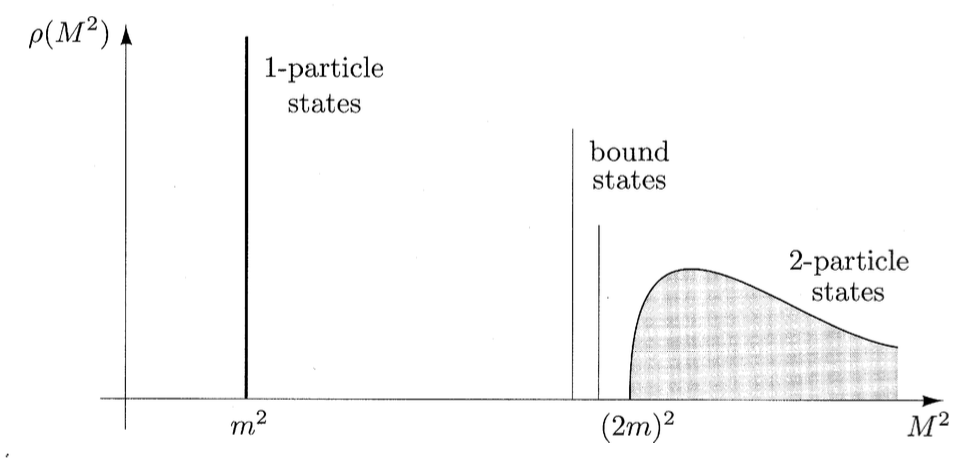
\includegraphics[scale=0.7]{spectral density.png}
  \caption{谱密度图示}
  \label{sd}
\end{figure}
谱密度函数在单粒子质量处有孤立的Delta函数,对于$ M>2m $处是连续的:
\begin{equation}
  \rho\left(M^2\right)=2 \pi \delta\left(M^2-m^2\right) \cdot Z+\left(\text { nothing else until } M^2 \gtrsim(2 m)^2\right)
\end{equation}
Z是由矩阵元平方求和给出的常数,称为场强重整化,m是单粒子的物理质量。\\

对位置空间的关联函数作傅立叶变换,有:
\begin{equation}
  \begin{aligned}
    \int d^4 x e^{i p \cdot x}\langle\Omega|T \phi(x) \phi(0)| \Omega\rangle & =\int_0^{\infty} \frac{d M^2}{2 \pi} \rho\left(M^2\right) \frac{i}{p^2-M^2+i \epsilon} \\
    & =\frac{i Z}{p^2-m^2+i \epsilon}+\int_{\sim 4 m^2}^{\infty} \frac{d M^2}{2 \pi} \rho\left(M^2\right) \frac{i}{p^2-M^2+i \epsilon}
    \end{aligned}
\end{equation}
可以看出,全传播子在物理质量处有极点。
\subsection{LSZ约化公式}
在上节可以看到,动量空间的两点关联函数作为$ p^2 $的解析函数,在单粒子态质量处有如下的极点结构:
\begin{equation}
  \int d^4 x e^{i p \cdot x}\langle\Omega|T \phi(x) \phi(0)| \Omega\rangle \underset{p^2 \rightarrow m^2}{\sim} \frac{i Z}{p^2-m^2+i \epsilon}
  \label{ps}
\end{equation} 
本节将上述结果推广到一般的关联函数,并由此给出关联函数与S矩阵元的关系。考虑一个$ 2\to n $过程,
对其中一个场作傅立叶变换,作为傅立叶变量p的函数具有\eqref{ps}的极点结构。将证明和这些极点关联
起来的单粒子态实际上是渐进态,即以某动量为中心,相隔很远的波包。取n+2个外线粒子在壳极限,可以将
多重极点的系数解释为S矩阵。\\

先对n+2点关联函数其中的一个变量作傅立叶变换,分析下述积分:
\begin{equation}
  \int d^4 x e^{i p \cdot x}\left\langle\Omega\left|T\left\{\phi(x) \phi\left(z_1\right) \phi\left(z_2\right) \cdots\right\}\right| \Omega\right\rangle
\end{equation}
要找出变量$ p^0 $的极点,讲积分拆为三部分:
\begin{equation}
  \int d x^0=\int_{T_{+}}^{\infty} d x^0+\int_{T_{-}}^{T_{+}} d x^0+\int_{-\infty}^{T_{-}} d x^0
\end{equation} 
$ T_+,T_- $分别远大/小于其他的时间$ z_i^0 $。将积分区域分别称为I,II,III,区域II是有界的,
且对$ p^0 $的依赖完全来自解析函数$ \exp(ip^0x^0) $,它的积分对于$ p^0$是解析的。I与III是无界
的,因此有可能产生奇异性。\\

考虑区域I,此处$ \phi(x) $在最前面,插入完备关系(单粒子真空态没有贡献):
\begin{equation}
  \begin{aligned}
    \int_{T_{+}}^{\infty} d x^0 \int d^3 x e^{i p^0 x^0} e^{-i \mathbf{p} \cdot \mathbf{x}} \sum_\lambda \int \frac{d^3 q}{(2 \pi)^3} & \frac{1}{2 E_{\mathbf{q}}(\lambda)}\left\langle\Omega|\phi(x)| \lambda_{\mathbf{q}}\right\rangle \\
    & \times\left\langle\lambda_{\mathbf{q}}\left|T\left\{\phi\left(z_1\right) \phi\left(z_2\right) \cdots\right\}\right| \Omega\right\rangle
    \end{aligned}
\end{equation} 
利用关系\eqref{rela}并插入收敛因子$e^{-\epsilon x^0}  $使得积分良定义,由此有:
\begin{equation}
  \begin{aligned}
    & \sum_\lambda \int_{T_{+}}^{\infty} d x^0 \int \frac{d^3 q}{(2 \pi)^3} \frac{1}{2 E_{\mathbf{q}}(\lambda)} e^{i p^0 x^0} e^{-i q^0 x^0} e^{-\epsilon x^0}\left\langle\Omega|\phi(0)| \lambda_0\right\rangle(2 \pi)^3 \delta^{(3)}(\mathbf{p}-\mathbf{q}) \\
    & \times\left\langle\lambda_{\mathbf{q}}\left|T\left\{\phi\left(z_1\right) \cdots\right\}\right| \Omega\right\rangle \\
    & =\sum_\lambda \frac{1}{2 E_{\mathbf{p}}(\lambda)} \frac{i e^{i\left(p^0-E_{\mathbf{p}}+i \epsilon\right) T_{+}}}{p^0-E_{\mathbf{p}}(\lambda)+i \epsilon}\left\langle\Omega|\phi(0)| \lambda_0\right\rangle\left\langle\lambda_{\mathbf{p}}\left|T\left\{\phi\left(z_1\right) \cdots\right\}\right| \Omega\right\rangle . 
    \end{aligned}
\end{equation} 
可以看出它具有如下极点结构:
\begin{equation}
  \begin{aligned}
    \int d^4 x e^{i p \cdot x}\left\langle\Omega\left|T\left\{\phi(x) \phi\left(z_1\right) \cdots\right\}\right| \Omega\right\rangle \\
    \underset{p^0 \rightarrow+E_{\mathbf{p}}}{\sim} \frac{i}{p^2-m^2+i \epsilon} \sqrt{Z}\left\langle\mathbf{p}\left|T\left\{\phi\left(z_1\right) \cdots\right\}\right| \Omega\right\rangle
    \end{aligned}
\end{equation}
相似地有III的贡献:
\begin{equation}
  \begin{aligned}
    \int d^4 x e^{i p \cdot x}\langle\Omega| & T\left\{\phi(x) \phi\left(z_1\right) \cdots\right\}|\Omega\rangle \\
    & \underset{p^0 \rightarrow-E_{\mathbf{p}}}{\sim}\left\langle\Omega\left|T\left\{\phi\left(z_1\right) \cdots\right\}\right|-\mathbf{p}\right\rangle \sqrt{Z} \frac{i}{p^2-m^2+i \epsilon}
    \end{aligned}
\end{equation}
对剩下的场做傅立叶变换,为防止不同粒子的干涉,取波包模型而非点粒子模型,对于傅立叶变换做出如下改变:
\begin{equation}
  \int d^4 x e^{i p^0 x^0} e^{-i \mathbf{p} \cdot \mathbf{x}} \rightarrow \int \frac{d^3 k}{(2 \pi)^3} \int d^4 x e^{i p^0 x^0} e^{-i \mathbf{k} \cdot \mathbf{x}} \varphi(\mathbf{k})
\end{equation}
$ \varphi(\mathbf{k}) $是表示一个集中在p动量的波包分布。因此,极点结构修正为:
\begin{equation}
  \begin{aligned}
    & \sum_\lambda \int \frac{d^3 k}{(2 \pi)^3} \varphi(\mathbf{k}) \frac{1}{2 E_{\mathbf{k}}(\lambda)} \frac{i}{p^0-E_{\mathbf{k}}(\lambda)+i \epsilon}\left\langle\Omega|\phi(0)| \lambda_0\right\rangle\left\langle\lambda_{\mathbf{k}}\left|T\left\{\phi\left(z_1\right) \cdots\right\}\right| \Omega\right\rangle\\
    & \underset{p^0 \rightarrow+E_{\mathbf{p}}}{\sim} \int \frac{d^3 k}{(2 \pi)^3} \varphi(\mathbf{k}) \frac{i}{\tilde{p}^2-m^2+i \epsilon} \sqrt{Z}\left\langle\mathbf{k}\left|T\left\{\phi\left(z_1\right) \cdots\right\}\right| \Omega\right\rangle
  \end{aligned}
\end{equation} 
此时奇异性从极点变为割线,可以通过缩小$ \varphi(\mathbf{k}) $代表的波包使得割线退化为极点。对关联
函数中所有的变量都做波包型变换:
\begin{equation}
  \left(\prod_i \int \frac{d^3 k_i}{(2 \pi)^3} \int d^4 x_i e^{i \tilde{p}_i \cdot x_i} \varphi_i\left(\mathbf{k}_i\right)\right)\left\langle\Omega\left|T\left\{\phi\left(x_1\right) \phi\left(x_2\right) \cdots\right\}\right| \Omega\right\rangle
\end{equation}
选取$ T_+,T_- $使得波包在I,III区域相隔很远,在x=0处接触。选择粒子1,2处于将来,它们在时序
乘积的前两项,再插入完备算符,此时有:
\begin{equation}
  \begin{aligned}
    & \sum_\lambda \int \frac{d^3 K}{(2 \pi)^3} \frac{1}{2 E_{\mathbf{K}}}\left(\prod_{i=1,2} \int \frac{d^3 k_i}{(2 \pi)^3} \int d^4 x_i e^{i \tilde{p}_i \cdot x_i} \varphi_i\left(\mathbf{k}_i\right)\right) \\
    & \times\left\langle\Omega\left|T\left\{\phi\left(x_1\right) \phi\left(x_2\right)\right\}\right| \lambda_{\mathbf{K}}\right\rangle\left\langle\lambda_{\mathbf{K}}\left|T\left\{\phi\left(x_3\right) \cdots\right\}\right| \Omega\right\rangle
    \end{aligned}
\end{equation}
态$ \lambda_{\mathbf{K}} $被两个相隔很远的波包湮灭,因此它必定对应真空中的两个独立激发,近似有:
\begin{equation}
  \begin{aligned}
    & \sum_\lambda \int \frac{d^3 K}{(2 \pi)^3} \frac{1}{2 E_{\mathbf{K}}}\left\langle\Omega\left|T\left\{\phi\left(x_1\right) \phi\left(x_2\right)\right\}\right| \lambda_{\mathbf{K}}\right\rangle\left\langle\lambda_{\mathbf{K}}\right| \\
    & =\sum_{\lambda_1 \lambda_0} \int \frac{d^3 q_1}{(2 \pi)^3} \frac{1}{2 E_{\mathbf{q}_1}} \int \frac{d^3 q_2}{(2 \pi)^3} \frac{1}{2 E_{\mathbf{q}_2}}\left\langle\Omega\left|\phi\left(x_1\right)\right| \lambda_{\mathbf{q}_1}\right\rangle\left\langle\Omega\left|\phi\left(x_2\right)\right| \lambda_{\mathbf{q}_2}\right\rangle\left\langle\lambda_{\mathbf{q}_1} \lambda_{\mathbf{q}_2}\right|
    \end{aligned}
\end{equation} 
对$ x_1,x_0 $的积分给出上节熟悉的极点结构:
\begin{equation}
  \left(\prod_{i=1,2} \int \frac{d^3 k_i}{(2 \pi)^3} \varphi_i\left(\mathbf{k}_i\right) \frac{i}{\tilde{p}_i^2-m^2+i \epsilon} \cdot \sqrt{Z}\right)\left\langle\mathbf{k}_1 \mathbf{k}_2\left|T\left\{\phi\left(x_3\right) \cdots\right\}\right| \Omega\right\rangle
\end{equation} 
取点粒子极限,并同样地处理其他场,有:
\begin{equation}
  \left(\prod_{i=1,2} \frac{i}{p_i{ }^2-m^2+i \epsilon} \cdot \sqrt{Z}\right)\left(\prod_{i=3, \ldots . .} \frac{i}{p_i{ }^2-m^2+i \epsilon} \cdot \sqrt{Z}\right)_{\text {out }}\left\langle\mathbf{p}_1 \mathbf{p}_2 \mid-\mathbf{p}_3 \cdots\right\rangle_{\mathrm{in}}
\end{equation}
由此可以得出结论:S矩阵元就是对应动量关联函数在多重极点处的系数。综上,LSZ公式为:
\begin{equation}
  \begin{array}{r}
    \prod_1^n \int d^4 x_i e^{i p_i \cdot x_i} \prod_1^m \int d^4 y_j e^{-i k_j \cdot y_j}\left\langle\Omega\left|T\left\{\phi\left(x_1\right) \cdots \phi\left(x_n\right) \phi\left(y_1\right) \cdots \phi\left(y_m\right)\right\}\right| \Omega\right\rangle \\
    \underset{\substack{\text { each } p_i^0 \rightarrow+E_{\mathbf{p}_i} \\
    \text { each } k_j^0 \rightarrow+E_{\mathbf{k}_j}}}{\sim}\left(\prod_{i=1}^n \frac{\sqrt{Z} i}{p_i^2-m^2+i \epsilon}\right)\left(\prod_{j=1}^m \frac{\sqrt{Z} i}{k_j^2-m^2+i \epsilon}\right)\left\langle\mathbf{p}_1 \cdots \mathbf{p}_n|S| \mathbf{k}_1 \cdots \mathbf{k}_m\right\rangle .
    \end{array}
\end{equation}
LSZ公式也解答了为什么计算S矩阵元只考虑了Amputated的图:简单来说,对于自能图我们要求它在粒子质量处
有对应的极点,每条外线的自能图都贡献这样一个极点,刚好就是我们前文所述的极点结构,而S矩阵元是极点的
系数,因此对应了Amputated的图。
\section{Noether定理与}
\subsubsection{粒子的Noether定理}
对一个广义坐标为$ q^i $的系统,对称定义为对任意$ q^i(t) $,下述方程总是满足的函数$ \delta q^i(t) $
\begin{equation}
  \delta I\left[q^i(t), \delta_s q^i(t)\right] \equiv I\left[q^i(t)+\delta_s q^i(t)\right]-I\left[q^i(t)\right]=\int d t \frac{d K}{d t}
\end{equation}
这与变分方程,要求$\delta I=0$对任意$ \delta q^i(t) $总成立,从而是关于广义坐标的方程恰好相反\footnote{满足此条件的就是E-L方程,而对$ q^i(t) $的方程并没有显式给出}
\begin{equation}
  \begin{aligned}
    \delta I\left[q^i, \delta q^i\right] & =\int d t\left(\frac{\partial L}{\partial q^i} \delta q^i+\frac{\delta L}{\delta \dot{q}^i} \delta \dot{q}^i\right) \\
    & =\int d t\left(\frac{\partial L}{\partial q^i}-\frac{d}{d t}\left(\frac{\partial L}{\partial \dot{q}^i}\right)\right) \delta q^i+\int d t \frac{d}{d t}\left(\frac{\partial L}{\partial \dot{q}^i} \delta q^i\right) .
    \end{aligned}
\end{equation}
当选取on-shell的$ q^i $时,两种方式的作用量变分相同,相减以后得到守恒量
\begin{equation}
  \frac{d}{d t} Q=0 \quad \text { with } \quad Q=K-\frac{\partial L}{\partial \dot{q}^i} \delta_s q^i
\end{equation}
\begin{center}
Noether第一定理:给定一个对称$ \delta q^i(t) $,上面定义的Q是守恒的
\end{center}
\subsubsection{哈密顿形式中的Noether定理}
在哈密顿形式中作用量为
\begin{equation}
  I\left[p_i, q^j\right]=\int d t\left(p_i \dot{q}^i-H(p, q)\right)
\end{equation}
一个量Q守恒即不随时间改变,意味着
\begin{equation}
  \frac{d Q(p, q, t)}{d t}=0 \quad \Rightarrow \quad[Q, H]+\frac{\partial Q}{\partial t}=0
\end{equation}
大多数时候我们考虑的Q不显含时间,因此泊松括号为零就给出守恒量,此时有如下定理
\begin{enumerate}
  \item Noether逆定理:如果Q是一个守恒量,如下定义的变换是一个对称变换
  \begin{equation}
    \delta_s q^i=\left[q^i, \epsilon Q\right]=\epsilon \frac{\partial Q}{\partial p_i} \quad, \quad \delta_s p_i=\left[p_i, \epsilon Q\right]=-\epsilon \frac{\partial Q}{\partial q^i}
  \end{equation}
  此处先给出守恒量,再给出对称变换,所以叫逆定理
  \item 对称的Lie代数:所有守恒量的集合$ {Q_a} $满足闭Lie代数
  \begin{equation}
    \left[Q_a, Q_b\right]=f_{a b}^c Q_c
  \end{equation} 
\end{enumerate}
可以验证上述变换确实是对称变换
\begin{equation}
  \begin{aligned}
    \delta I & =\int d t\left(\delta_s p \dot{q}+p \frac{d}{d t} \delta_s q-\frac{\partial H}{\partial p} \delta_s p-\frac{\partial H}{\partial q} \delta_s q\right) \\
    & =\int d t\left(-\epsilon \frac{\partial Q}{\partial q} \dot{q}+\frac{d}{d t}\left(p \delta_s q\right)-\epsilon \dot{p} \frac{\partial Q}{\partial p}+\epsilon \frac{\partial H}{\partial p} \frac{\partial Q}{\partial q}-\epsilon \frac{\partial H}{\partial q} \frac{\partial Q}{\partial p}\right) \\
    & =\int d t\left(\epsilon\left(-\frac{d Q}{d t}+\frac{\partial Q}{\partial t}+[Q, H]\right)+\frac{d}{d t}\left(p \delta_s q\right)\right) \\
    & =\int d t \frac{d}{d t}\left(-\epsilon Q+p \delta_s q\right),
    \end{aligned}
\end{equation}
由于守恒量之间的泊松括号也是守恒量,因此持续使用泊松括号最终总会得到闭的Lie代数
\subsubsection{场的Noether定理}
对场的对称变换定义为
\begin{equation}
  \delta I\left[\phi, \delta_s \phi\right] \equiv I\left[\phi+\delta_s \phi\right]-I[\phi]=\int d^d x \partial_\mu K^\mu \quad \forall \phi
\end{equation}
这同样是关于场的无限小变换函数$ \delta \varphi $的方程。注意,此处场函数的自变量$ x $ 并没有出现,因为它是“哑指标”,总是被积去,关于时空的变换会诱导出场的变换,而正是场的变换才是这里所考虑的。\\
同样的,通过考虑on-shell场的无穷小对称变换,可以得到守恒方程
\begin{center}
\begin{equation}
  \partial_\mu J^\mu=0 \quad \text { where } \quad J^\mu \equiv \frac{\partial \mathcal{L}}{\partial \phi_{, \mu}} \delta \phi(x)-K^\mu
  \label{FNT}
\end{equation}
\end{center} 
只要场随距离衰减地足够快\footnote{对于规范场这不成立},可以抛去边界项定义守恒量
\begin{equation}
  Q=\int_V d^3 x J^0(x) \quad \text { with } \quad \frac{d}{d t} Q=0
\end{equation}
现在仔细考虑坐标变换对场的影响。一般来说,坐标变换后新场与原场的关系为
\begin{equation}
\begin{aligned}
\phi^{\prime}\left(x^{\prime}\right) & =\phi(x) \\
V^{\prime \mu}\left(x^{\prime}\right) & =\frac{\partial x^{\prime \mu}}{\partial x^\nu} V^\nu(x) \\
A_\mu^{\prime}\left(x^{\prime}\right) & =\frac{\partial x^\nu}{\partial x^{\prime \mu}} A_\nu(x) \\
g_{\mu \nu}^{\prime}\left(x^{\prime}\right) & =\frac{\partial x^\alpha}{\partial x^{\prime \mu}} \frac{\partial x^\beta}{\partial x^{\prime \nu}} g_{\alpha \beta}(x)
\end{aligned}
\end{equation}
对于Noether定理,我们希望考虑无限小变换,这对应
\begin{equation}
  x^\mu=x^\mu+\xi^\mu(x) \quad \Rightarrow \quad \frac{\partial x^{\prime \mu}}{\partial x^\nu}=\delta_\nu^\mu+\partial_\nu \xi^\mu(x) \quad, \quad \frac{\partial x^\mu}{\partial x^{\prime \nu}}=\delta_\nu^\mu-\partial_\nu \xi^\mu\left(x^{\prime}\right)
\end{equation}
而此时标量场的无限小变换为
\begin{equation}
  \delta \phi(x)=\phi^{\prime}(x)-\phi(x)=-\xi^\nu(x) \partial_\nu \phi(x) .
\end{equation}
这刚好就是沿着矢量场$ \xi^\mu(x) $ Lie导数的定义,对于其他场也有类似的结果
\begin{equation}
  \begin{aligned}
    \mathcal{L}_{\xi} \phi & =-\xi^\nu \partial_\nu \phi(x) \\
    \mathcal{L}_{\xi} A_\mu & =-\xi^\alpha \partial_\alpha A_\mu-A_\alpha \partial_\mu \xi^\alpha \\
    \mathcal{L}_{\xi} g_{\mu \nu} & =-\xi^\alpha \partial_\alpha g_{\mu \nu}(x)-g_{\mu \beta}(x) \partial_\nu \xi^\beta-g_{\alpha \nu}(x) \partial_\mu \xi^\alpha
    \end{aligned}
\end{equation}
所以对于时空对称性,并不是说在坐标变换下作用量不变,因为这只是一个变量代换,积分的值当然不变,而是说坐标变换下由场的Lie导数表示的场的无限小变换下作用量不变。
\subsubsection{能动张量}
能动张量的一个定义为时空平移$ x^\mu \rightarrow x^\mu+\epsilon^\mu $ 对应的守恒流。由场的Noether定理给出守恒流的形式为$ J^\mu=T_\nu^\mu \epsilon^\nu $\footnote{\eqref{FNT}给出的守恒流正比于无穷小变换的参量,此处无穷下变换的参量是一个矢量,而流也是矢量,因此还需与一个张量缩并}\\
对于标量场,对称变换给出
\begin{equation}
  \delta \mathcal{L}=\frac{\partial \mathcal{L}}{\partial \phi} \delta \phi+\frac{\partial \mathcal{L}}{\partial \phi,,_\rho} \delta \phi,{ }_\rho=-\epsilon^\sigma\left[\frac{\partial \mathcal{L}}{\partial \phi} \phi,{ }_\sigma+\frac{\partial \mathcal{L}}{\partial \phi,{ }_\rho} \phi,{ }_{\rho \sigma}\right]=-\partial_\sigma\left(\epsilon^\sigma \mathcal{L}\right)
\end{equation}
因此对应的守恒流和能动张量为
\begin{equation}
  J^\mu=\epsilon^\rho\left[\frac{\partial \mathcal{L}}{\partial \phi,{ }_{, \mu}} \partial_\rho \phi-\delta_\rho^\mu \mathcal{L}\right] \equiv \epsilon^\rho T_\rho^\mu
\end{equation}
\begin{equation}
  T^\mu{ }_\nu(x)=\frac{\partial \mathcal{L}}{\partial \phi_{, \mu}} \partial_\rho \phi-\delta_\rho^\mu \mathcal{L} \quad \text { with } \quad \partial_\mu T_\rho^\mu=0
\end{equation}
\subsubsection{第二Noether定理与规范对称性}
\href{https://physics.stackexchange.com/questions/66092/noether-charge-of-local-symmetries}{Noether charge of local symmetries}
考虑一个不包含场的高阶导数的拉氏量$ \mathcal{L}=\mathcal{L}(\phi(x), \partial \phi(x), x) $,虽然推导过程一直使用拉氏量,但形式上定义正则动量$ \pi_\alpha^\mu:=\frac{\partial \mathcal{L}}{\partial\left(\partial_\mu \phi^\alpha\right)} $ ,$ \alpha $表示可能出现的不同的场。记E-L方程为
\begin{equation}
  E_\alpha:=\frac{\partial \mathcal{L}}{\partial \phi^\alpha}-\partial_\mu \pi_\alpha^\mu
\end{equation}  
现在考虑由时空相关的参数$ \varepsilon(x) $标记的场的无穷小变化,并且不考虑关于$ \varepsilon $的高阶项以及高阶导数
\begin{equation}
  \delta_{\varepsilon} \phi^\alpha=Y^\alpha(\varepsilon)=Y^\alpha \varepsilon+Y^{\alpha, \mu} \partial_\mu \varepsilon
\end{equation}
参数$ Y^\alpha,Y^{\alpha, \mu} $都不依赖于$ \varepsilon $。定义部分Noether流$ j^\mu(\varepsilon) $ 为正则动量与场的无穷小变化的乘积
\begin{equation}
  \begin{gathered}
    j^\mu \varepsilon+j^{\mu, \nu} \partial_\nu \varepsilon=j^\mu(\varepsilon):=\pi_\alpha^\mu Y^\alpha(\varepsilon) \\
    j^\mu:=\pi_\alpha^\mu Y^\alpha, \quad j^{\mu, \nu}:=\pi_\alpha^\mu Y^{\alpha, \nu} .
    \end{gathered}
\end{equation}
如果这个场的无穷小变化是一个对称变换,那么它会使得哈密顿量密度在相差一个全散度项的意义下不变

\begin{equation}
  \begin{aligned}
  & \text { chain } \\
  & d_\mu f^\mu(\varepsilon)=\delta_{\varepsilon} \mathcal{L} \stackrel{\text { rule }}{=} \frac{\partial \mathcal{L}}{\partial \phi^\alpha} Y^\alpha(\varepsilon)+\pi_\alpha^\mu \partial_\mu Y^\alpha(\varepsilon) \\
  & \text { Leibniz' } \\
  & \stackrel{\text { rule }}{=} \quad E_\alpha Y^\alpha(\varepsilon)+\partial_\mu j^\mu(\varepsilon) . \\
  &
  \end{aligned}
  \label{7}
  \end{equation}
    


我们同样将f展开为系数与$ \varepsilon $无关的形式,比较等号两边关于$ \varepsilon $的阶数,可知f包含$ \varepsilon $的二阶导数
\begin{equation}
  f^\mu(\varepsilon)=f^\mu \varepsilon+f^{\mu, \nu} \partial_\nu \varepsilon+\frac{1}{2} f^{\mu, \nu \lambda} \partial_\nu \partial_\lambda \varepsilon
\end{equation}   
定义完整Noether流$ J^\mu(\varepsilon) $ 为
\begin{equation}
  J^\mu \varepsilon+J^{\mu, \nu} \partial_\nu \varepsilon+\frac{1}{2} J^{\mu, \nu \lambda} \partial_\nu \partial_\lambda \varepsilon=J^\mu(\varepsilon):=j^\mu(\varepsilon)-f^\mu(\varepsilon)
  \label{10}
\end{equation}
由\eqref{7}、\eqref{10}可以得到一个off-shell成立的等式
\begin{equation}
  \partial_\mu J^\mu(\varepsilon)=-E_\alpha Y^\alpha(\varepsilon)  
\end{equation}
将$ \varepsilon $及其导数的系数逐项相等,可以得到如下一系列等式
\begin{equation}
  \begin{gathered}
    \partial_\mu J^\mu=-E_\alpha Y^\alpha, \\
    J^\mu+\partial_\nu J^{\nu, \mu}=-E_\alpha Y^{\alpha, \mu}, \\
    J^{\nu, \lambda}+J^{\lambda, \nu}+\partial_\mu J^{\mu, \nu \lambda}=0, \\
    \sum_{\text {cycl. } \mu, \nu, \lambda} J^{\mu, \nu \lambda}=0,
    \end{gathered}
\end{equation} 
第一项在令$ \varepsilon $与时空无关时仍然存在,因此它就是我们喜闻乐见的物理的on-shell守恒流(a.k.a第一Noether流)。剩下的项可以用来定义第二Noether流$ \mathcal{J}^\mu(\varepsilon) $ 
\begin{equation}
  \mathcal{J}^\mu \varepsilon+\mathcal{J}^{\mu, \nu} \partial_\nu \varepsilon+\frac{1}{2} \mathcal{J}^{\mu, \nu \lambda} \partial_\nu \partial_\lambda \varepsilon=\mathcal{J}^\mu(\varepsilon):=J^\mu(\varepsilon)+E_\alpha Y^{\alpha, \mu} \varepsilon
\end{equation}
它的守恒律是off-shell的,因此给出系统的一个约束
\begin{equation}
  \begin{gathered}
    \partial_\mu \mathcal{J}^\mu(\varepsilon) =-E_\alpha Y^\alpha(\varepsilon)+d_\mu\left(E_\alpha Y^{\alpha, \mu} \varepsilon\right) \\
    =-\varepsilon d_\mu d_\nu J^{\nu, \mu} = \frac{\varepsilon}{2} \partial_\mu d_\nu \partial_\lambda J^{\lambda, \mu \nu} = 0
    \end{gathered}
\end{equation}
并且可以定义一个Superpotential满足$ \partial_\nu \mathcal{K}^{\mu \nu}(\varepsilon)=\mathcal{J}^\mu(\varepsilon) $,如果我们要求$ \mathcal{J}^\mu(\varepsilon) $在时空无穷远处趋于零,那么对应的守恒荷总是零
\begin{equation}
  \mathcal{Q}(\varepsilon):=\int_V d^3 V \mathcal{J}^0(\varepsilon)=\int_V d^3 V \partial_i \mathcal{K}^{0 i}(\varepsilon)=\int_{\partial V} d^2 A_i \mathcal{K}^{0 i}(\varepsilon)=0
\end{equation}  
总而言之,将local对称性限制在global给出物理的守恒荷,剩下流的部分满足off-shell守恒并且守恒荷为零,off-shell成立的方程相当于是对于系统的一个约束。

\section{Ward Identity, david tong, gauge theory p130}
现在考察Noether定理在量子场论中的情况。一个场的变换对于配分函数来说只是积分变量的替换,不会改变积分值,因此此时我们应该定义对称为使得如下等式成立的场变换
\begin{equation}
  \mathcal{D} \phi \exp{-S[\phi]} = \mathcal{D} \phi^\prime = \exp{-S[\phi^\prime]}
\end{equation}
此时,对于一个算符f的期望值与其对称变换后$ f\circ g $ 的有关系:
\begin{equation}
  <f>=<f\circ g>
\end{equation}
对于所有对称性,一个算符在原本场的配分函数下的期望值和这个算符写在对称变换后的场但仍是原本场的配分函数下期望值相等。\\
现在用无限小变换改写上面的内容。考虑一个global对称性,它使得场在如下无限小变换后作用量不变

  \begin{equation}
    \Phi^{\prime}(x)=\Phi(x)-i \omega_a G_a \Phi(x)
    \end{equation}

$ G_a $是生成元。现在将$ \omega_a $提升为$ \omega_a(x) $并 考虑一个关于场$ \Phi $的量X,它的期望值可以在变换前后的场分别写出
\begin{equation}
    \begin{aligned}
    \left\langle X \right\rangle & =\frac{1}{Z} \int[\mathcal{D} \Phi] X(\Phi) \exp -S[\Phi] \\
    & =\frac{1}{Z} \int\left[\mathcal{D} \Phi^{\prime}\right] X(\Phi^{\prime}) \exp -S\left[\Phi^{\prime}\right] \\
    & =\frac{1}{Z} \int[\mathcal{D} \Phi] X+\delta_w X \exp {-S[\Phi]+\int d x \partial_\mu j_a^\mu \omega_a(\boldsymbol{x})} \\
    & =\left\langle X \right\rangle + \left\langle \delta_w X \right\rangle +\left\langle \partial_\mu j_a^\mu \omega_a(\boldsymbol{x}) \right\rangle
    \end{aligned}
\end{equation}
上面假设了场的测度在这个变换下不变,并在最后一个等式展开了指数项并且只保留了$ \omega $的一阶项。若X为一系列场的乘积,那么它在场无穷小变换下的变换保留至$ \omega $的一阶项为
\begin{equation}
  \begin{aligned}
    \delta X & =-i \sum_{i=1}^n\left(\Phi\left(x_1\right) \cdots G_a \Phi\left(x_i\right) \cdots \Phi\left(x_n\right)\right) \omega_a\left(x_i\right) \\
    & =-i \int d x \omega_a(x) \sum_{i=1}^n\left\{\Phi\left(x_1\right) \cdots G_a \Phi\left(x_i\right) \cdots \Phi\left(x_n\right)\right\} \delta\left(x-x_i\right)
    \end{aligned}
\end{equation}
上述等式对于任何$ \omega_a(x) $总是成立,因此可以将积分内的项直接相等,于是得到ward identity。
\begin{center}

\boxed{  
  \begin{aligned}
    & \frac{\partial}{\partial x^\mu}\left\langle j_a^\mu(x) \Phi\left(x_1\right) \cdots \Phi\left(x_n\right)\right\rangle \\
    & \quad=-i \sum_{i=1}^n \delta\left(x-x_i\right)\left\langle\Phi\left(x_1\right) \cdots G_a \Phi\left(x_i\right) \cdots \Phi\left(x_n\right)\right\rangle
    \end{aligned}
  }
\end{center}

\section{外场与有效作用量}
\subsection{来自热力学的类比}
考虑一个磁性系统,配分函数以及Helmholtz自由能为:
\begin{equation}
  Z(H)=e^{-\beta F(H)}=\int \mathcal{D} s \exp \left[-\beta \int d x(\mathcal{H}[s]-H s(x))\right]
\end{equation}
$ H $为外加磁场。磁化强度可以通过对Helmholtz自由能求导得到:
\begin{equation*}
  \begin{aligned}
    -\left.\frac{\partial F}{\partial H}\right|_{\beta \text { fixed }} & =\frac{1}{\beta} \frac{\partial}{\partial H} \log Z \\
    & =\frac{1}{Z} \int d x \int \mathcal{D} s s(x) \exp \left[-\beta \int d x(\mathcal{H}[s]-H s)\right] \\
    & =\int d x\langle s(x)\rangle \equiv M .
    \end{aligned}
\end{equation*}
Gibbs自由能 通过Legendre变换得到
\begin{equation*}
  G=f+MH
\end{equation*}
外场可以对Gibbs自由能 求导得到:
\begin{equation}
  \begin{aligned}
    \frac{\partial G}{\partial M} & =\frac{\partial F}{\partial M}+M \frac{\partial H}{\partial M}+H \\
    & =\frac{\partial H}{\partial M} \frac{\partial F}{\partial H}+M \frac{\partial H}{\partial M}+H \\
    & =H
    \end{aligned}
\end{equation}
当$ H=0 $时,Gibbs自由能 取极值,热力学上最稳定的态由$ G(M) $的最小值给出。通过类比,我们也可以在QFT中构造相似的量,为方便仅考虑标量场。
\subsection{有效作用量的引入}
 标量场的生成函数为:
 \begin{equation}
  Z[J]=e^{-i E[J]}=\int \mathcal{D} \phi \exp \left[i \int d^4 x(\mathcal{L}[\phi]+J \phi)\right]
 \end{equation}
 一般而言通常的记号并非$ E(J) $,而是$ W(J) $,后文中可能交替使用两种记号。可以看出$ E(J) $可以类比Helmholtz自由能 ,它的物理意义是
 真空-真空振幅的联通部分。J类比外磁场。之后的讨论中我们假定J是均匀的,通过泛函的一些技巧我们很容易推广到一般的场。\\
 令$ E(J) $对J求泛函导数,有:
 \begin{equation}
  \frac{\delta}{\delta J(x)} E[J]=i \frac{\delta}{\delta J(x)} \log Z=-\frac{\int \mathcal{D} \phi e^{i \int(\mathcal{L}+J \phi)} \phi(x)}{\int \mathcal{D} \phi e^{i \int(\mathcal{L}+J \phi)}}
 \end{equation}  
将上式简记为:
\begin{equation}
  \frac{\delta}{\delta J(x)} E[J]=-\langle\Omega|\phi(x)| \Omega\rangle_J
\end{equation}
等式右侧为有场J时$ \phi $的真空期望。注意到热力学中和外场共轭的物理量也是内场的平均值,因此我们定义:
\begin{equation}
  \phi_{\mathrm{cl}}(x)=\langle\Omega|\phi(x)| \Omega\rangle_J
  \label{defofcf}
\end{equation}
由此定义Gibbs自由能 的QFT类比,即$ E(J) $的Legendre变换
\footnote{在Weinberg等教材中,此处的Legendre变换定义略有不同,并没有取场在源J的真空期望值作为Legendre变换中和J共轭的量
,而是定义$ J_{\phi 人} $为产生期望值为$ \phi^r $的流,再定义Legendre变换:
\begin{equation}
  \Gamma[\phi] \equiv-\int \mathrm{d}^4 x \phi^r(x) J_{\phi r}(x)+W\left[J_\phi\right]
  \label{defofw}
\end{equation}  
后文在计算有效作用量时主要采用了这个定义}
\\
\begin{equation}
  \Gamma\left[\phi_{\mathrm{cl}}\right] \equiv-E[J]-\int d^4 y J(y) \phi_{\mathrm{cl}}(y)
  \label{defofea}
\end{equation} 
对经典场再求泛函导数,有:
\begin{equation}
  \begin{aligned}
    \frac{\delta}{\delta \phi_{\mathrm{cl}}(x)} \Gamma\left[\phi_{\mathrm{cl}}\right] & =-\frac{\delta}{\delta \phi_{\mathrm{cl}}(x)} E[J]-\int d^4 y \frac{\delta J(y)}{\delta \phi_{\mathrm{cl}}(x)} \phi_{\mathrm{cl}}(y)-J(x) \\
    & =-\int d^4 y \frac{\delta J(y)}{\delta \phi_{\mathrm{cl}}(x)} \frac{\delta E[J]}{\delta J(y)}-\int d^4 y \frac{\delta J(y)}{\delta \phi_{\mathrm{cl}}(x)} \phi_{\mathrm{cl}}(y)-J(x) \\
    & =-J(x) .
    \end{aligned}
\end{equation}
热力学和QFT的类比总结如图\ref*{Analog}:\\
\begin{figure}[htp]
  \centering
  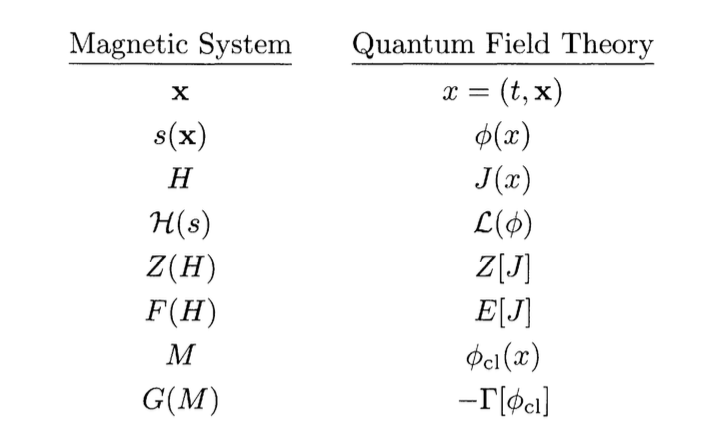
\includegraphics[scale=0.8]{analog.png}
  \caption{热力学与QFT类比}
  \label{Analog}
\end{figure}
很容易看出,当外场为零时,有:
\begin{equation}
  \frac{\delta}{\delta \phi_{\mathrm{cl}}(x)} \Gamma\left[\phi_{\mathrm{cl}}\right]=0
  \label{ec}
\end{equation}
此方程的解就是理论中的稳定构型。对于平移不变的真空态,解是不依赖于x的,但有时也会有额外的解称为瞬子。\\
在此假设考虑的理论中可能的真空态在平移以及Lorentz变换下总是不变的,此时方程变为非常简单的非泛函方程,进一步我们知道
$ \Gamma $是一个广延量,它正比于我们所选取的时空体积:
\begin{equation}
  \Gamma\left[\phi_{\mathrm{cl}}\right]=-(V T) \cdot V_{\mathrm{eff}}\left(\phi_{\mathrm{cl}}\right)
\end{equation} 
系数$ V_{\mathrm{eff}}\left(\phi_{\mathrm{cl}}\right) $称为有效势。$ \Gamma\left[\phi_{\mathrm{cl}}\right] $
取极值的条件简化为$ V_{\mathrm{eff}}\left(\phi_{\mathrm{cl}}\right) $取极值。
\subsection{有效作用量的性质}
先给出结论:我们知道$ Z[J] $是关联函数的生成泛函,而$ \Gamma\left[\phi_{\mathrm{cl}}\right] $ 是单粒子不可约关联函数
的生成泛函。为看出这一点,从两点关联函数算起。
\begin{equation}
  \begin{aligned}
    & \frac{\delta^2 E[J]}{\delta J(x) \delta J(y)}=-\frac{i}{Z} \int \mathcal{D} \phi e^{i \int(\mathcal{L}+J \phi)} \phi(x) \phi(y) \\
    & \quad+\frac{i}{Z^2} \int \mathcal{D} \phi e^{i \int(\mathcal{L}+J \phi)} \phi(x) \cdot \int \mathcal{D} \phi e^{i \int(\mathcal{L}+J \phi)} \phi(y) \\
    &=-i[\langle\phi(x) \phi(y)\rangle-\langle\phi(x)\rangle\langle\phi(y)\rangle] .
    \end{aligned}
\end{equation}
 非连通部分刚好被抵消,对更高阶的泛函导数也有相同的结果(link cluster theorem),因此有:
 \begin{equation}
  \frac{\delta^n E[J]}{\delta J\left(x_1\right) \cdots \delta J\left(x_n\right)}=(i)^{n+1}\left\langle\phi\left(x_1\right) \cdots \phi\left(x_n\right)\right\rangle_{\mathrm{conn}}
 \end{equation}
 现在开始考虑$ \gamma $,对\eqref{ec}求场$ J(y) $的泛函导数有:
 \begin{equation*}
  \frac{\delta}{\delta J(y)} \frac{\delta \Gamma}{\delta \phi_{\mathrm{cl}}(x)}=-\delta(x-y)
 \end{equation*} 
 利用链式法则展开左式:
 \begin{equation}
  \begin{aligned}
    \delta(x-y) & =-\int d^4 z \frac{\delta \phi_{\mathrm{cl}}(z)}{\delta J(y)} \frac{\delta^2 \Gamma}{\delta \phi_{\mathrm{cl}}(z) \delta \phi_{\mathrm{cl}}(x)} \\
    & =\int d^4 z \frac{\delta^2 E}{\delta J(y) \delta J(z)} \frac{\delta^2 \Gamma}{\delta \phi_{\mathrm{cl}}(z) \delta \phi_{\mathrm{cl}}(x)} \\
    & =\left(\frac{\delta^2 E}{\delta J \delta J}\right)_{y z}\left(\frac{\delta^2 \Gamma}{\delta \phi_{\mathrm{cl}} \delta \phi_{\mathrm{cl}}}\right)_{z x}
    \end{aligned}
    \label{2p}
 \end{equation}
 可以看到这两个无限维矩阵互为逆:
 \begin{equation}
  \left(\frac{\delta^2 E}{\delta J \delta J}\right)=\left(\frac{\delta^2 \Gamma}{\delta \phi_{\mathrm{cl}} \delta \phi_{\mathrm{cl}}}\right)^{-1}
 \end{equation}
 已知左式为连通两点关联函数,即传播子,因此右式为传播子的逆。到动量空间可以更容易看出物理意义:
 \begin{equation*}
  \widetilde{D}^{-1}(p)=-i\left(p^2-m^2-M^2\left(p^2\right)\right)
 \end{equation*}
 $ M^2\left(p^2\right) $是自能函数,是所有单粒子不可约两点图的求和。进一步求泛函导数,用链式法则改写求导:
 \begin{equation*}
  \frac{\delta}{\delta J(z)}=\int d^4 w \frac{\delta \phi_{\mathrm{cl}}(w)}{\delta J(z)} \frac{\delta}{\delta \phi_{\mathrm{cl}}(w)}=i \int d^4 w D(z, w) \frac{\delta}{\delta \phi_{\mathrm{cl}}(w)}
 \end{equation*}
 并利用矩阵逆求导的法则:
 \begin{equation*}
  \frac{\partial}{\partial \alpha} M^{-1}(\alpha)=-M^{-1} \frac{\partial M}{\partial \alpha} M^{-1}
 \end{equation*}
 继续对\eqref{2p}求泛函导数,有:
 \begin{equation*}
  \begin{aligned}
    \frac{\delta^3 E[J]}{\delta J_x \delta J_y \delta J_z} & =i \int d^4 w D(z, w) \frac{\delta}{\delta \phi_w^{\mathrm{cl}}}\left(\frac{\delta^2 \Gamma}{\delta \phi_x^{\mathrm{cl}} \delta \phi_y^{\mathrm{cl}}}\right)^{-1} \\
    & =i \int d^4 w D_{z w}(-1) \int d^4 u \int d^4 v\left(-i D_{x u}\right) \frac{\delta^3 \Gamma}{\delta \phi_u^{\mathrm{cl}} \delta \phi_v^{\mathrm{cl}} \delta \phi_w^{\mathrm{cl}}}\left(-i D_{v y}\right)\\
    & =i \int d^4 u d^4 v d^4 w D_{x u} D_{y v} D_{z w} \frac{\delta^3 \Gamma}{\delta \phi_u^{\mathrm{cl}} \delta \phi_v^{\mathrm{cl}} \delta \phi_w^{\mathrm{cl}}}
  \end{aligned}
 \end{equation*}
 \begin{figure}[htp]
  \centering
  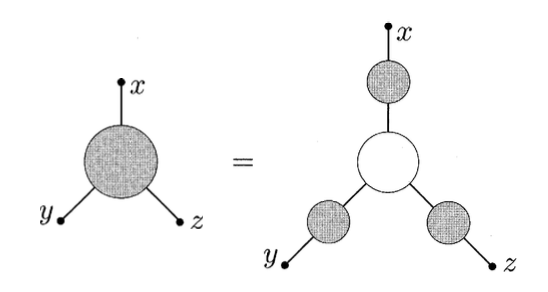
\includegraphics[scale=1]{3DR.png}
  \caption{三点关系的图像表示}
  \label{3DR}
\end{figure}
深灰圈表示连通图的求和,浅灰圈表示量子作用量的三阶泛函导数,可以看出它代表所有完全传播子移除后的连通三点关联函数,
即单粒子不可约三点函数:
\begin{equation*}
  \frac{i \delta^3 \Gamma}{\delta \phi_{\mathrm{cl}}(x) \phi_{\mathrm{cl}}(y) \phi_{\mathrm{cl}}(z)}=\langle\phi(x) \phi(y) \phi(z)\rangle_{1 \mathrm{PI}}
\end{equation*}
继续求导,可以总结出以下关系:
\begin{equation}
  \frac{\delta^n \Gamma\left[\phi_{\mathrm{cl}}\right]}{\delta \phi_{\mathrm{cl}}\left(x_1\right) \cdots \delta \phi_{\mathrm{cl}}\left(x_n\right)}=-i\left\langle\phi\left(x_1\right) \cdots \phi\left(x_n\right)\right\rangle_{1 \mathrm{PI}}
\end{equation}
因此我们得出,量子有效作用量是单粒子不可约关联函数的生成泛函。因此,类比$ W(J) $是所有连通真空-真空图的求和,$ \Gamma[\phi_{cl}] $是所有单粒子不可约
连通图的求和。 \\
若将生成泛函中的经典作用量$ I[\phi] $直接换成量子有效作用量$ \Gamma[\phi] $,则有:
\begin{equation}
  Z_{\Gamma}[j]=e^{W_{\Gamma}[j]}=\int[D \phi(x)] \exp \left[i \Gamma[\phi(x)]+i \int d^4 x j(x) \phi(x)\right]
\end{equation}   
我们将证明,这个生成泛函所代表的真空-真空振幅的连通树图部分给出了原本经典作用量$ I[\phi] $的理论的所有阶贡献。为分离出
树图部分,引入一个常数试图标记不同部分的贡献:
\begin{equation}
  Z_r[j ; \hbar]=e^{w_r[j ; \hbar]}=\int[D \phi(x)] \exp \left[\frac{i}{\hbar}\left(\Gamma[\phi(x)]+\int d^4 x j(x) \phi(x)\right)\right]
\end{equation}
传播子给出贡献$ \hbar $,顶点给出贡献$ \hbar^{-1} $,又拓扑恒等式,圈数$ n_L $、内线数I,顶点数V有关系$ n_L=I-V+1 $,
因此L圈图的贡献正比于$ \hbar^{n_L-1} $,形式上可以有:
\begin{equation}
  W_{\Gamma}[j ; \hbar]=\sum_{n_L=0}^{\infty} \hbar^{n_L-1} \underbrace{W_{\Gamma, n_L}[j]}_{n_L \text { loops }}
\end{equation}     
为分离出树图,形式上取极限$ \hbar\to 0 $,此时圈图贡献趋于零,且路径积分由稳相点主导。 
\subsection{有效作用量的计算}
我们在重整微扰论的框架下,从定义式\eqref{defofea}出发,逐阶计算泛函。首先,照常把拉氏量写为两部分:
\begin{equation}
  \mathcal{L}=\mathcal{L}_1+\delta \mathcal{L}
\end{equation}
把流分为两部分$ J(x)=J_1(x)+\delta J(x) $ ,其中一部分满足如下方程:
\begin{equation}
  \left.\frac{\delta \mathcal{L}_1}{\delta \phi}\right|_{\phi=\phi_{\mathrm{cl}}}+J_1(x)=0
  \label{defofj1}
\end{equation}
而$ \delta J(x) $的取值是的总的流让场的真空期望值仍是$ \phi_{cl}(x) $ 即$ \langle\phi(x)\rangle_J=\phi_{\mathrm{cl}}(x) $\\
现在生成泛函为:
\begin{equation}
  Z[J]=\int \mathcal{D} \phi e^{i \int d^4 x\left(\mathcal{L}_1[\phi]+J_1 \phi\right)} e^{i \int d^4 x(\delta \mathcal{L}[\phi]+\delta J \phi)}
\end{equation}
平移场的定义,取$ \phi(x)=\phi_{\mathrm{cl}}(x)+\eta(x) $ ,指数中的项做幂级数展开:
\begin{equation}
  \begin{aligned}
    \int d^4 x\left(\mathcal{L}_1+J_1 \phi\right) & =\int d^4 x\left(\mathcal{L}_1\left[\phi_{\mathrm{cl}}\right]+J_1 \phi_{\mathrm{cl}}\right)+\int d^4 x \eta(x)\left(\frac{\delta \mathcal{L}_1}{\delta \phi}+J_1\right) \\
    & +\frac{1}{2} \int d^4 x d^4 y \eta(x) \eta(y) \frac{\delta^2 \mathcal{L}_1}{\delta \phi(x) \delta \phi(y)} \\
    & +\frac{1}{3 !} \int d^4 x d^4 y d^4 z \eta(x) \eta(y) \eta(z) \frac{\delta^3 \mathcal{L}_1}{\delta \phi(x) \delta \phi(y) \delta \phi(z)}+\cdots
    \end{aligned}
\end{equation}
一阶项由\eqref{defofj1}直接为零,二阶项给出高斯积分,高阶项视作微扰修正。暂且忽略抵消项与高阶修正,高斯积分给出有效作用量的第一个修正项:
\begin{equation}
  \begin{aligned}
    \int \mathcal{D} \eta & \exp \left[i\left(\int\left(\mathcal{L}_1\left[\phi_{\mathrm{cl}}\right]+J_1 \phi_{\mathrm{cl}}\right)+\frac{1}{2} \int \eta \frac{\delta^2 \mathcal{L}_1}{\delta \phi \delta \phi} \eta\right)\right] \\
    = & \exp \left[i \int\left(\mathcal{L}_1\left[\phi_{\mathrm{cl}}\right]+J_1 \phi_{\mathrm{cl}}\right)\right] \cdot\left(\operatorname{det}\left[-\frac{\delta^2 \mathcal{L}_1}{\delta \phi \delta \phi}\right]\right)^{-1 / 2} .
    \end{aligned}
\end{equation}
高阶项的作用在Feynman图表示中,给出了一系列以$ -i\left(\frac{\delta^2 \mathcal{L}_1}{\delta \phi \delta \phi}\right)^{-1} $ 
作为传播子,高阶项作为顶点的Feynman规则图。\\
考虑抵消项,也在$ \phi_{cl} $处展开,有 
\begin{equation}
  \left(\delta \mathcal{L}\left[\phi_{\mathrm{cl}}\right]+\delta J \phi_{\mathrm{cl}}\right)+\left(\delta \mathcal{L}\left[\phi_{\mathrm{cl}}+\eta\right]-\delta \mathcal{L}\left[\phi_{\mathrm{cl}}\right]+\delta J \eta\right)
\end{equation}
第二项Taylor展开后也给出Feynman图修正,第一项是一个常数。总结,有效作用量为:
\begin{equation}
  \begin{aligned}
    \Gamma\left[\phi_{\mathrm{cl}}\right]= & \int d^4 x \mathcal{L}_1\left[\phi_{\mathrm{cl}}\right]+\frac{i}{2} \log \operatorname{det}\left[-\frac{\delta^2 \mathcal{L}_1}{\delta \phi \delta \phi}\right] \\
    & -i \cdot(\text { connected diagrams })+\int d^4 x \delta \mathcal{L}\left[\phi_{\mathrm{cl}}\right]
    \end{aligned}
\end{equation}
上述连通图都是真空-真空图,至少也是两圈图,因此最低阶修正就是泛函行列式。上面的构造中比正常的重整化多了一个抵消项:$ \delta J $,它由
下述方法给出:\\
首先在头阶项有关系$ \langle\phi\rangle=\phi_{\mathrm{cl}} $,此等式会因为Feynman图给出的修正而不成立,且贡献都来自于
“蝌蚪”图,他们刚好可以由$ \delta J\eta $项抵消是的等式依然成立。在实际操纵中我们直接忽略连通单粒子不可约单点图,因为刚好被
$ \delta J\eta $抵消。
\subsection{有效作用量的对称性}
虽然不总是这样, 但在某些情况下, 作用量$ I[\phi] $ 的对称性自动地也是有效作用量的$ \Gamma[\phi] $ 的对称性。除非我们能够证明附加于作用量的对称性也适用于有效作用量, 否则我们在建立理论的可重 整性时会遇到问题。\\
为此没我们研究一种重要的对称性,它由如下无限小变换生成:
\begin{equation}
  \chi^n(x) \rightarrow \chi^n(x)+\epsilon F^n[x ; \chi]
\end{equation}
假定测度和作用量在变换下都不变:
\begin{equation}
  \begin{aligned}
    I[\chi+\epsilon F] & =I[\chi] \\
    \prod_{n, x} \mathrm{~d}\left(\chi^n(x)+\epsilon F[x ; \chi]\right) & =\prod_{n, x} \mathrm{~d} \chi^n(x)
    \end{aligned}
\end{equation}
此时生成泛函为:
\begin{equation}
  \begin{aligned}
    Z[J]= & \int\left[\prod_{n, x} \mathrm{~d}\left(\chi^n(x)+\epsilon F^n[x ; \chi]\right)\right] \\
    & \times \exp \left\{\mathrm{i} I[\chi+\epsilon F]+\mathrm{i} \int \mathrm{d}^4 x\left(\chi^n(x)+\epsilon F^n[x ; \chi]\right) J_n(x)\right\} \\
    = & \int\left[\prod_{n, x} \mathrm{~d} \chi^n(x)\right] \exp \left\{\mathrm{i} I[\chi]+\mathrm{i} \int \mathrm{d}^4 x\left(\chi^n(x)+\epsilon F^n[x ; \chi]\right) J_n(x)\right\} \\
    = & Z[J]+\mathrm{i} \epsilon \int\left(\prod_{n, x} \mathrm{~d} \chi^n(x)\right) \int F^n(y ; \chi) J_n(y) \mathrm{d}^4 y \\
    & \times \exp \left\{\mathrm{i} I[\chi]+\mathrm{i} \int \mathrm{d}^4 x \chi^n(x) J_n(x)\right\}
    \end{aligned}
\end{equation}
上式中Taylor展开了指数项。因此:
\begin{equation}
  \int \mathrm{d}^4 y\left\langle F^n(y)\right\rangle_J J_n(y)=0
\end{equation}
回忆起在此定义下流由此式给出:
\begin{equation}
  J_{n, \chi}(y)=-\frac{\delta \Gamma[\chi]}{\delta \chi^n(y)}
\end{equation}
因此有:
\begin{equation}
  0=\int \mathrm{d}^4 y\left\langle F^n(y)\right\rangle_{J_\chi} \frac{\delta \Gamma[\chi]}{\delta \chi^n(y)}
\end{equation}
也即$ \Gamma[\chi] $在无限小变换
\begin{equation}
  \chi^n(y) \rightarrow \chi^n(y)+\epsilon\left\langle F^n(y)\right\rangle_{J_\chi}
\end{equation} 
下不变,这样的对称性调教被称为Slavnov-Taylor恒等式。若我们出发的无限小变换时线性变换那两者时相同的。
\section{量子Goldstone定理}

QFT中的Goldstone定理证明与经典场类似,只不过势能换成有效势。为说明这一点,需要引入一些关于有效作用量的结论.
\subsection{寻找真空}
我们知道,量子有效作用量在场的真空期望值处取极值:
\begin{equation}
  \left(\frac{\delta \Gamma[\phi]}{\delta \phi(x)}\right)_{\phi=\langle\Omega|\phi| \Omega\rangle}=0
\end{equation}
为找出真空态$ |\Psi> $,它需要使得哈密顿量期望值最小,并且对场的期望值给出上述极值条件的解,还要满足归一性,利用Lagrange乘数法
求解这个约束极值问题,可以转化为最小化以下的量:
\begin{equation}
  \langle\Psi|H| \Psi\rangle-A\langle\Psi \mid \Psi\rangle-\int d^3 x B(\mathbf{x})\langle\Psi|\phi(\mathbf{x})| \Psi\rangle
\end{equation} 
对量子态变分取极值,给出条件:
\begin{equation}
  H|\Psi\rangle=A|\Psi\rangle+\int d^3 x B(\mathbf{x}) \phi(\mathbf{x})|\Psi\rangle
\end{equation}
\begin{equation}
  \left(H-\int d^3 x J(\mathbf{x}) \phi(\mathbf{x})\right)\left|\Psi_J\right\rangle=E[J]\left|\Psi_J\right\rangle
\end{equation}
原则上A、B的值也需要求极值得出,最终结果以泛函的关系依赖于场的期望值$ \phi_0{x0} $,但可以通过一种取巧的方式找到A、B。\\
考虑含流哈密顿量的基态本征方程:
\begin{equation}
  \left(H-\int d^3 x J(\mathbf{x}) \phi(\mathbf{x})\right)\left|\Psi_J\right\rangle=E[J]\left|\Psi_J\right\rangle
\end{equation}
若取$ B=J_0:=J_{\phi_0}, A=E\left[J_{\phi_0}\right] $,则$ \left|\Psi_J\right\rangle $ 满足约束条件且能量取极值。\\
为得到有效作用量与能量的关系,考虑这样一个过程:$ -\infty\to +\infty $过程中,逐渐光滑地打开源,并维持恒定的$ J(\vec{x}) $时间T,最后再光滑地撤去源。\\
真空-真空振幅会积累一个相因子:
\begin{equation}
  \langle\Omega, \infty \mid \Omega,-\infty\rangle_J=\exp (-i E[J] T)
\end{equation}
于是有关系:$ W[J]=-E[J] T $。回到没有外源的原本理论,它的真空态由下列方程给出:
\begin{equation}
  \begin{aligned}
    H\left|\Psi_{J_0}\right\rangle&=\left(E[J_0]+\int d^3 x J_0(\mathbf{x}) \phi_0(\mathbf{x})\right)\left|\Psi_{J_0}\right\rangle\\
    &=\frac{1}{T}\left(-W\left[J_0\right]+\int d^4 x J_0(x) \phi_0(x)\right)\left|\Psi_{J_0}\right\rangle\\
    &=-\frac{\Gamma\left[\phi_0\right]}{T}\left|\Psi_{J_0}\right\rangle
  \end{aligned}
\end{equation}
也就是说,对于期望值为$ \phi_0 $的场构型的态,它的能量与该场构型对应的量子作用量只相差一个负系数。满足极值条件的场构型
中,是的量子作用量最大值的就对应能量的最低点,即真空态。 \\

我们总希望真空仍就具有Poincare群的对称性,因此场的期待值是一个常数,从而量子作用量的展开中含导数项的都为零,只剩下了
$ V_{eff} $称为有效势$ \Gamma\left[\phi_0\right]=-V T V_{\mathrm{eff}}\left(\phi_0\right) $,此时寻求真空
就变成了寻求有效势的极值,而在最低阶近似下有效势就是拉氏量中的经典势。
\subsection{简并真空}
经典中基态简并,系统由于历史或者各种微扰处于某个确定的破缺对称性的基态是容易理解的,但由于量子
系统的线性可加,需要额外的论述。事实上,只有无限大的量子系统才能有自发对称破缺。\\

考虑最简单的一个对称性,反射对称性:$ \phi \rightarrow-\phi $ ,此时基态二重简并,$ |\mathrm{VAC},+\rangle,|\mathrm{VAC},-\rangle $
都是对称破缺的基态,但$ |\mathrm{VAC},\rangle\pm |\mathrm{VAC},+\rangle $ 仍具有对称性。 
假设哈密顿量的真空矩阵元为:
\begin{equation}
  \begin{aligned}
    & \langle\mathrm{VAC},+|H| \mathrm{VAC},+\rangle=\langle\mathrm{VAC},-|H| \mathrm{VAC},-\rangle \equiv a \\
    & \langle\mathrm{VAC},+|H| \text { VAC },-\rangle=\langle\mathrm{VAC},-|H| \mathrm{VAC},+\rangle \equiv b
    \end{aligned}
\end{equation}
此时l两者的线性组合才是本征态,且对称不变。真空态之间的隧穿概率可以由下式得出:
\begin{equation}
  \left\langle\Omega_{+}\left|e^{i H t}\right| \Omega_{-}\right\rangle \approx e^{-S_E}=e^{-V \int_0^t \mathcal{L}_E\left(\phi_{\mathrm{cl}}\right) d t}
\end{equation}
$ S_E $为wick转动以后的欧几里得作用量,上述过程取了鞍点近似,积分一般为一有限值,因此空间
体积将指数压缩隧穿概率。 此时两个$ \pm $线性组合态高度简并。考虑破坏对称性的微扰,它将解除
简并,使得$ \mathrm{VAC},\pm\rangle $成为本征值不同的本征态,物理真空具体是谁取决于微扰
本身,但只要它比原本的哈密顿量小很多就不重要。当系统体积有限时,微扰对矩阵元的贡献远小于“隧穿”
对非对角元的贡献,此时基态仍是对称的叠加态,也就是说没有发生对称破缺。 
\subsection{量子Goldstone定理的证明}  
\paragraph*{Proof\: 1}
第一个证明与之前经典的情况几乎完全一致,只需补充几个小细节。我们假设作用量以及测度再一个连续
对称变化下都不变,它的代表,无限小变换时线性的:
\begin{equation}
  \phi_n(x) \rightarrow \phi_n(x)+\mathrm{i} \epsilon \sum_m t_{n m} \phi_m(x)
\end{equation}
由之前的论证,作用量线性的对称性在量子作用量中仍然保持,因此有关系:
\begin{equation*}
  \sum_{n, m} \int \frac{\delta \Gamma[\phi]}{\delta \phi_n(x)} t_{n m} \phi_m(x) \mathrm{d}^4 x=0
\end{equation*}
再考虑平移不变理论,作用量的形式为$ \Gamma[\phi]=-\mathscr{V} V(\phi) $,不变条件可以改写为:
\begin{equation*}
  \sum_{n, m} \frac{\partial V(\phi)}{\partial \phi_n} t_{n m} \phi_m=0
\end{equation*}
再次对场球道,并且利用极值条件,给出关系:
\begin{equation*}
  \left.\sum_{n, m} \frac{\partial^2 V(\phi)}{\partial \phi_n \partial \phi_{\ell}}\right|_{\phi=\bar{\phi}} t_{n m} \bar{\phi}_m=0
\end{equation*}
在经典的情况中,势能二阶导矩阵的本征值直接被认为是质量。有效势的二阶导如有效作用量节
所述,是单粒子不可约两点图之和,直接与动量空间的完全传播子的导数联系:
\begin{equation*}
  \frac{\partial^2 V(\phi)}{\partial \phi_n \partial \phi_{\ell}}=\Delta_{n \ell}^{-1}(0)
\end{equation*}
因此方程改写为:
\begin{equation*}
  \sum_{n, m} \Delta_{n \ell}^{-1}(0) t_{n m} \bar{\phi}_m=0
\end{equation*}
当对称性破缺时,$ \sum_m t_{n m} \bar{\phi}_m $不为零,此时它是$ \Delta_{n \ell}^{-1}(0) $
本征值为零的本征矢,若对角化,$ \phi_{Gm}=U_{nm}\phi_{m} $,$U_{mn}$为使得矩阵对角化的变换
,n取为零本征值对应的下标。这意味着$ \Delta_{n \ell}^{-1}(q) $在$ q^2=0 $处有一极点,
因此无质量。\\

为看出Goldstone粒子属于洛伦兹群的哪个表示,我们先假设场$ \phi_\alpha $对应
表示D,于是有$ \phi_\alpha^{\prime}=D_{\alpha \beta}(\Lambda) \phi_\beta $。Goldstone子
与原本场的线性关系可能让人误以为他们对应相同的表示,但U在Lorentz变化下并不平庸,为看出这一点,
传播子的倒数按照$ D^{-1}\otimes D^{-1} $变换 ,对角化后的矩阵为Lorentz标量矩阵,因此变换矩阵
按照$ D^{-1} $变换,刚好抵消的原本场的变换,因此Goldstone粒子是零自旋玻色子。
\paragraph*{Proof\: 2}
任何连续对称性都给出一个守恒流$ J^{\mu} $,以及相应的守恒荷Q,并且这个Q诱导对应的对称变换:
\begin{equation*}
  Q=\int \mathrm{d}^3 x J^0(\mathbf{x}, 0)
\end{equation*} 
\begin{equation*}
  \left[Q, \phi_n(x)\right]=-\sum_m t_{n m} \phi_m(x)
\end{equation*}
上述算符关系不受自发对称性破缺的影响。现在考察流和场的对易子的真空期望值,并对中间态求和,有:
\begin{equation}
  \left\langle\left[J^\lambda(y), \phi_n(x)\right]\right\rangle_{\mathrm{VAC}}=(2 \pi)^{-3} \int \mathrm{d}^4 p\left[\rho_n^\lambda(p) \mathrm{e}^{\mathrm{i} p \cdot(y-x)}-\tilde{\rho}_n^\lambda(p) \mathrm{e}^{\mathrm{i} p \cdot(x-y)}\right]
\end{equation}
其中利用平移不变形,以及插入完备关系定义了:
\begin{equation}
  \begin{aligned}
    & (2 \pi)^{-3} \mathrm{i} \rho_n^\lambda(p)=\sum_N\left\langle\operatorname{VAC}\left|J^\lambda(0)\right| N\right\rangle\left\langle N\left|\phi_n(0)\right| \mathrm{VAC}\right\rangle \delta^4\left(p-p_N\right), \\
    & (2 \pi)^{-3} \mathrm{i} \tilde{\rho}_n^\lambda(p)=\sum_N\left\langle\operatorname{VAC}\left|\phi_n(0)\right| N\right\rangle\left\langle N\left|J^\lambda(0)\right| \operatorname{VAC}\right\rangle \delta^4\left(p-p_N\right) .
    \end{aligned}
\end{equation}
对N的求和表示对所有离散的指标求和以及对连续指标的积分。由于$ \rho $是动量四矢的函数,且自身
有一个Lorentz矢量指标,因此正比于$ p^\mu $,而插入完备集中的态能量总是正定的,因此也正比
于能量的阶梯函数,即:
\begin{equation}
  \begin{aligned}
    & \rho_n^\lambda(p)=p^\lambda \rho_n\left(-p^2\right) \theta\left(p^0\right) \\
    & \tilde{\rho}_n^\lambda(p)=p^\lambda \tilde{\rho}_n\left(-p^2\right) \theta\left(p^0\right)
    \end{aligned}
\end{equation}  
真空期望可以改写为:
\begin{equation}
  \begin{aligned}
    \left\langle\left[J^\lambda(y), \phi_n(x)\right]\right\rangle_{\mathrm{VAC}}= & \frac{\partial}{\partial y_\lambda} \int \mathrm{d} \mu^2\left[\rho_n\left(\mu^2\right) \Delta_{+}\left(y-x ; \mu^2\right)\right. \\
    & \left.+\tilde{\rho}_n\left(\mu^2\right) \Delta_{+}\left(x-y ; \mu^2\right)\right]
    \end{aligned}
\end{equation}
其中:$  \Delta_{+}\left(z ; \mu^2\right)=(2 \pi)^{-3} \int \mathrm{d}^4 p \theta\left(p^0\right) \delta\left(p^2+\mu^2\right) \mathrm{e}^{\mathrm{i} p \cdot z}$。\\

当$ z^2>0 $时,Lorentz不变形要求$ \Delta_{+}\left(z ; \mu^2\right) $仅能依赖于$ z^2、\mu^2 $。
因此$ \Delta_{+}\left(z ; \mu^2\right) $关于$ (x-y) $在类空时是偶函数,此时:
\begin{equation}
  \left\langle\left[J^\lambda(y), \phi_n(x)\right]\right\rangle_{\mathrm{VAC}}=\frac{\partial}{\partial y_\lambda} \int \mathrm{d} \mu^2\left[\rho_n\left(\mu^2\right)+\tilde{\rho}_n\left(\mu^2\right)\right] \Delta_{+}\left(y-x ; \mu^2\right)
\end{equation}    
由因果关系,类空对易子必为零给出条件:
\begin{equation}
  \rho_n\left(\mu^2\right)=-\tilde{\rho}_n\left(\mu^2\right)
\end{equation}
而对于一般的x,y,代入上式给出:
\begin{equation}
  \left\langle\left[J^\lambda(y), \phi_n(x)\right]\right\rangle_{\mathrm{VAC}}=\frac{\partial}{\partial y_\lambda} \int \mathrm{d} \mu^2 \rho_n\left(\mu^2\right)\left[\Delta_{+}\left(y-x ; \mu^2\right)-\Delta_{+}\left(x-y ; \mu^2\right)\right]
\end{equation}
为利用流守恒条件,两边同时再对$ Y^\lambda $求导,利用性质:
\begin{equation*}
  \left(\square_y-\mu^2\right) \Delta_{+}\left(y-x ; \mu^2\right)=0
\end{equation*} 
于是,对于任意的x和y,有:
\begin{equation}
  0=\int \mathrm{d} \mu^2 \mu^2 \rho_n\left(\mu^2\right)\left[\Delta_{+}\left(y-x ; \mu^2\right)-\Delta_{+}\left(x-y ; \mu^2\right)\right]
\end{equation}
只能有:
\begin{equation}
  \mu^2 \rho_n\left(\mu^2\right)=0
\end{equation}
此方程的解要么为$ rho_n\left(\mu^2\right)=0 $,要么为$ rho_n\left(\mu^2\right)\propto\delta(\mu^2) $。
我们将看到,对于对称破缺情况,只能为后者。
令$ \lambda=0,x^0=y^0=0 $,则有:
\begin{equation}
  \begin{aligned}
    \left\langle\left[J^0(\mathbf{y}, t), \phi_n(\mathbf{x}, t)\right]\right\rangle_{\text {VAC }}= & 2 \mathrm{i}(2 \pi)^{-3} \int \mathrm{d} \mu^2 \rho_n\left(\mu^2\right) \\
    & \times \int \mathrm{d}^4 p \sqrt{\mathbf{p}^2+\mu^2} \mathrm{e}^{\mathrm{i} \mathbf{p} \cdot(\mathbf{y}-\mathbf{x})} \theta(p_0)\delta\left(p^2+\mu^2\right) \\
    = & \mathrm{i} \delta^3(\mathbf{y}-\mathbf{x}) \int \mathrm{d} \mu^2 \rho_n\left(\mu^2\right) .
    \end{aligned}
\end{equation} 
其中用到了公式:$ \int_{-\infty}^{+\infty} d k^0 \delta\left(k^2+m^2\right) \theta\left(k^0\right)=\frac{1}{2 \omega} $ 。
对y空间积分,利用荷Q生成了这个对称变换,给出:
\begin{equation}
  -\sum_m t_{n m}\left\langle\phi_m\right\rangle_{\mathrm{VAC}}=\mathrm{i} \int \mathrm{d} \mu^2 \rho_n\left(\mu^2\right)
\end{equation}
仅当
\begin{equation}
  \rho_n\left(\mu^2\right)=\mathrm{i} \delta\left(\mu^2\right) \sum_m t_{n m}\left\langle\phi_m(0)\right\rangle_{\mathrm{VAC}}
\end{equation}
可以看出,对称破缺时,$ \rho_n\left(\mu^2\right) $不能为零,但正比于$ \delta\left(\mu^2\right) $的项职能出现在无质量粒子
的理论中,而且必须是单粒子态,因为多粒子态会给出连续的贡献。态$  \phi_n(0)|\mathrm{VAC}\rangle$是旋转
不变的\footnote{这似乎依赖$ \phi $是标量场 },因此呢只有螺旋度为零的态对$ \left\langle N\left|\phi_n(0)\right| \text { VAC }\right\rangle $
有贡献,同时只有内禀宇称以及内部量子数同$ J_0 $相同的态N对$ \left\langle V A C\left|J^0\right| N\right\rangle $有贡献,
因此呢Goldstone粒子是一个自旋为零的无质量粒子,且与$ J_0 $有相同的宇称以及内部量子数。     


\bibliographystyle{IEEEtran}
\bibliography{Ref}
\end{document}
